\chapter{Lattice dynamics}\label{chap:5}

Dark matter lighter than \SI{0.33}{MeV} cannot carry an electron of silicon across the \SI{1.17}{eV} gap (\cref{sec:3.3}), yet the crystal still has excitations that this light dark matter can reach. The nuclei vibrate at energies up to \SI{64}{meV}. By the bound $2\omega/v_{\mathrm{max}}^2$ of \cref{sec:1.3}, a vibrational quantum of \SI{64}{meV} is kinematically allowed for dark-matter masses down to about \SI{18}{keV}, and the acoustic vibrations reach lower masses still. \Cref{chap:3,chap:4} held the nuclei fixed and computed the response of the electrons alone, so the dynamic structure factor built there contains no vibrations of the nuclei. Letting the nuclei move raises questions that the static lattice could not ask. What potential do the nuclei move in, if the electrons that bind them also respond to their motion? How far does each nucleus stray from its site, even at a millikelvin, where zero-point motion is all there is? And what does a dark-matter particle that pushes on one nucleus set in motion in the whole crystal? The answers follow from the mass ratio $m_e/M \approx 2\times10^{-5}$, which separates the slow nuclei from the fast electrons and makes the vibrations of a crystal a nearly harmonic problem in a potential that density-functional theory computes. From the mass ratio we will build, in the steps of \cref{fig:5-map}, the phonons of silicon and of polar crystals, with their quanta, correlations and lifetimes; every nuclear-recoil and phonon rate of the later chapters takes these quantities as input.

\begin{figure}[tbp]
  \centering
  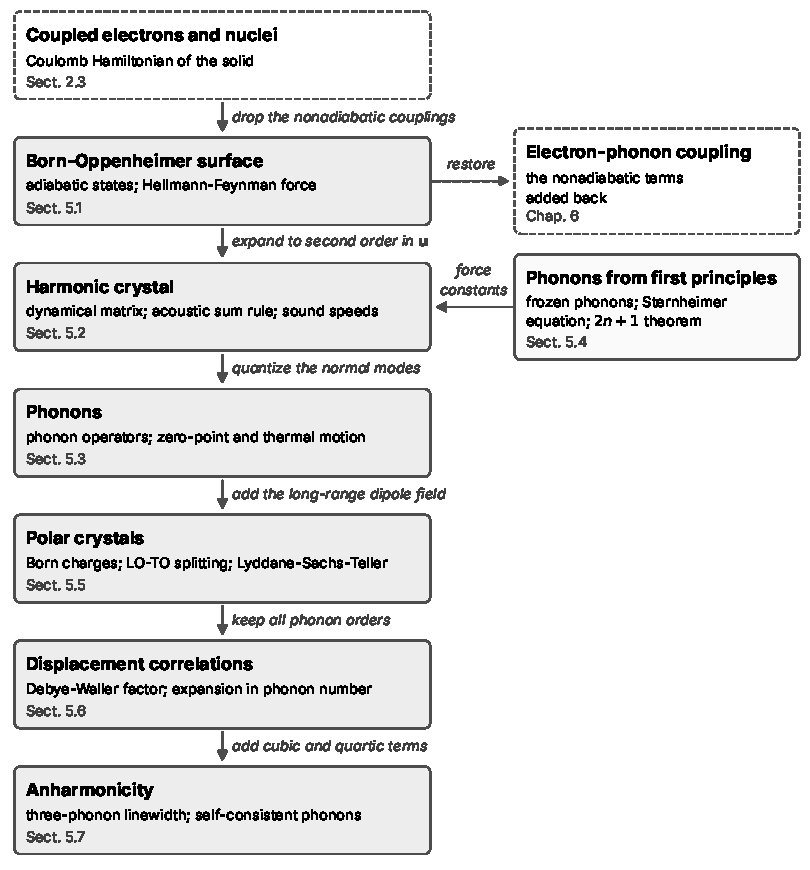
\includegraphics[width=0.85\linewidth]{figures/ch05/map05.pdf}
  \caption{From coupled electrons and nuclei to the anharmonic crystal. Dropping the nonadiabatic couplings gives the Born--Oppenheimer surface (\cref{sec:5.1}), and \cref{chap:6} restores the dropped couplings; expanding the surface to second order in the displacements gives the harmonic crystal (\cref{sec:5.2}); quantizing its normal modes gives phonons (\cref{sec:5.3}). The long-range dipole field adds the Born charges and LO--TO splitting of polar crystals (\cref{sec:5.5}); keeping all phonon orders gives the displacement correlations, the Debye--Waller factor and the multiphonon expansion (\cref{sec:5.6}); cubic and quartic terms give linewidths and self-consistent phonons (\cref{sec:5.7}). Dashed box: the force constants computed as a density response (\cref{chap:25}).}
  \label{fig:5-map}
\end{figure}

\section{The Born--Oppenheimer approximation}\label{sec:5.1}

The optical phonon of silicon at the zone center vibrates at \SI{15.5}{THz}~\cite{nilsson1972study}, an energy of \SI{64.1}{meV} and a period of \SI{64.5}{fs}. An electron excited across the gap of \SI{1.17}{eV} evolves on the time $2\pi/\Eg = \SI{3.5}{fs}$, eighteen times faster. During one swing of the nuclei the electrons have time to settle, many times over, into the lowest state compatible with where the nuclei happen to be. The crystal then behaves as the static lattice of \cref{sec:3.1} with the nuclei now allowed to move, slowly. This separation of the slow nuclei from the fast electrons is due to Born and Oppenheimer~\cite{born1927quantentheorie}, in the form that Born and Huang gave it for crystals~\cite[App.~VIII]{born1954dynamical}; the derivations of this section are written out in \cref{app:D.13}.

\subsection{Adiabatic states}

We start from the Coulomb Hamiltonian of electrons and point nuclei, \cref{eq:2.3-HC}. In a crystal it is natural to label the nucleus $I$ of \cref{sec:2.3} by its cell and its place in the cell. In the cell at the Bravais vector $\vect{R}$, the nucleus of species $\kappa$ sits at
\begin{equation}
  \vect{X}_I = \vect{R} + \vect{\tau}_\kappa + \vect{u}_{\vect{R}\kappa} ,
  \label{eq:5.1-X}
\end{equation}
where $\vect{\tau}_\kappa$ is its basis position in the cell (\cref{sec:3.1}) and $\vect{u}_{\vect{R}\kappa}$ its displacement. We write $u$ for the set of all displacements and $\nabla_{\vect{R}\kappa} = \partial/\partial\vect{u}_{\vect{R}\kappa}$. The equilibrium positions, about which $u$ is measured, are fixed below. Of the terms of \cref{eq:2.3-HC}, only the kinetic energy of the nuclei contains $\nabla_{\vect{R}\kappa}$. We separate it from the rest,
\begin{equation}
  H = -\sum_{\vect{R}\kappa}\frac{\nabla_{\vect{R}\kappa}^2}{2M_\kappa} + H_{\mathrm{el}}(u), \qquad
  H_{\mathrm{el}}(u) = T_e + V_{ee} + V_{eN}(u) + V_{NN}(u) ,
  \label{eq:5.1-H}
\end{equation}
with $T_e$ the kinetic energy of the electrons, the first term of \cref{eq:2.3-HC}, and $V_{ee}$, $V_{eN}$ and $V_{NN}$ the electron--electron, electron--nucleus and nucleus--nucleus terms of the bracket of \cref{eq:2.3-HC}. At fixed $u$, $H_{\mathrm{el}}(u)$ acts on the electron coordinates alone, which we collect in $r$, and the displacements $u$ enter $H_{\mathrm{el}}(u)$ as a set of parameters. The eigenstates of $H_{\mathrm{el}}(u)$ are the \emph{adiabatic states},
\begin{equation}
  H_{\mathrm{el}}(u)\,\Psi_i(r;u) = E_i(u)\,\Psi_i(r;u) ,
  \label{eq:5.1-adiabatic}
\end{equation}
orthonormal at every $u$. Each is a state of all the electrons with the nuclei held at the positions $u$. In the absence of a magnetic field $H_{\mathrm{el}}$ is real and the $\Psi_i$ can be chosen real, which we assume.

The adiabatic states are complete in $r$ at each $u$, and an exact state of electrons and nuclei can be expanded in them with $u$-dependent coefficients,
\begin{equation*}
  \Psi(r,u) = \sum_i\Psi^{\mathrm{nuc}}_i(u)\,\Psi_i(r;u) .
\end{equation*}
The coefficients $\Psi^{\mathrm{nuc}}_i$ are nuclear wavefunctions, one for each electronic state, and so far nothing has been approximated. Inserting the expansion into $H\Psi = E\Psi$ and projecting on $\Psi_j$ at fixed $u$ (\cref{app:D.13}) leads to coupled equations for the nuclear wavefunctions,
\begin{equation}
  \Bigl[-\sum_{\vect{R}\kappa}\frac{\nabla_{\vect{R}\kappa}^2}{2M_\kappa} + E_j(u)\Bigr]\Psi^{\mathrm{nuc}}_j + \sum_i\mathcal{N}_{ji}\,\Psi^{\mathrm{nuc}}_i = E\,\Psi^{\mathrm{nuc}}_j ,
  \label{eq:5.1-coupled}
\end{equation}
in which the electronic states couple to each other only through the operators
\begin{equation}
  \mathcal{N}_{ji} = -\sum_{\vect{R}\kappa}\frac{1}{2M_\kappa}\Bigl[2\,\langle\Psi_j|\nabla_{\vect{R}\kappa}\Psi_i\rangle\cdot\nabla_{\vect{R}\kappa} + \langle\Psi_j|\nabla_{\vect{R}\kappa}^2\Psi_i\rangle\Bigr] .
  \label{eq:5.1-N}
\end{equation}
These are the \emph{nonadiabatic couplings}: the first-derivative (or derivative) coupling, which acts on the nuclear wavefunction through $\nabla_{\vect{R}\kappa}$, and the second-derivative (or scalar) coupling. The brackets are integrals over $r$ and functions of $u$. Both couplings exist because the electronic state changes as the nuclei move, and both carry the factor $1/M_\kappa$.

The \emph{Born--Oppenheimer approximation} drops the nonadiabatic couplings. The electrons then stay in one adiabatic state (for an insulator at low temperature, the ground state), and the nuclei move in its energy:
\begin{equation}
  \Bigl[-\sum_{\vect{R}\kappa}\frac{\nabla_{\vect{R}\kappa}^2}{2M_\kappa} + E^{\mathrm{ad}}(u)\Bigr]\Psi^{\mathrm{nuc}}_0 = E\,\Psi^{\mathrm{nuc}}_0 , \qquad
  E^{\mathrm{ad}}(u) \equiv E_0(u) , \qquad
  \Psi \simeq \Psi^{\mathrm{nuc}}_0(u)\,\Psi_0(r;u) .
  \label{eq:5.1-BO}
\end{equation}
The ground-state energy of the electrons at fixed nuclei, with the repulsion of the nuclei included, has become the potential energy of the nuclei. It is the \emph{potential-energy surface}, or Born--Oppenheimer energy surface, $E^{\mathrm{ad}}(u)$, a function of the $3n_{\mathrm{at}}N$ nuclear coordinates for a crystal of $N$ cells, each with $n_{\mathrm{at}}$ nuclei. The physical picture is a slow nucleus pulling a cloud of electrons that rearranges instantly: the electrons follow the nuclei adiabatically, never get excited, and pass to the nuclei only the energy of their ground state. The rest of this chapter treats phonons, from their frequencies to their anharmonic decay, and every result it obtains is a statement about the shape of $E^{\mathrm{ad}}$ and about quantum mechanics on that surface. Born and Huang keep the diagonal term $\mathcal{N}_{00}$ as a small correction to $E^{\mathrm{ad}}$ and call the result the adiabatic approximation~\cite[App.~VIII]{born1954dynamical}. The field uses ``adiabatic'' and ``Born--Oppenheimer'' interchangeably, and so do we, since $\mathcal{N}_{00}$ is negligible (\cref{app:D.13}). The off-diagonal couplings $\mathcal{N}_{j\ne0,0}$ are what let a moving nucleus excite the electrons; they are the subject of \cref{sec:6.1}.

In a density-functional code, $E^{\mathrm{ad}}$ at a given set of nuclear positions is the Kohn--Sham total energy plus the repulsion of the nuclei (evaluated as an Ewald sum), and every code prints it as its standard output. Evaluating $E^{\mathrm{ad}}$ at displaced positions is the frozen-phonon method, and density-functional perturbation theory (\cref{sec:5.4}) computes the derivatives of $E^{\mathrm{ad}}$ at equilibrium directly. The Born--Oppenheimer approximation enters these calculations at one point only: the electrons are kept in their ground state at every configuration of the nuclei~\cite[Sect.~III\,A]{giustino2017electron}.

\subsection{Equilibrium positions and clamped nuclei}

The nuclei of a crystal at rest sit at a minimum of the energy surface. We choose the equilibrium positions $\vect{R} + \vect{\tau}_\kappa$ so that $u = 0$ is that minimum, $\nabla_{\vect{R}\kappa}E^{\mathrm{ad}} = 0$ for every nucleus. In silicon, each atom of the diamond structure sits at a site of tetrahedral symmetry, and the only vector that every operation of the tetrahedral group leaves unchanged is zero, so no atom feels a force at any lattice constant. The only free parameter is the lattice constant itself. Minimizing $E^{\mathrm{ad}}$ per cell with respect to the lattice constant yields \SI{5.401}{\angstrom} in the local-density approximation~\cite[Sect.~10.2]{ponce2016epw} and \SI{5.477}{\angstrom} in the PBE calculation of \cref{sec:3.4}, against the measured \SI{5.431}{\angstrom} (\cref{sec:3.1}). The lattice constant at the minimum of $E^{\mathrm{ad}}$ is not exactly the lattice constant that a diffraction experiment measures, since the zero-point spread of the nuclei on an anharmonic surface shifts the mean lattice constant away from the minimum (\cref{sec:5.7}).

\Cref{chap:3,chap:4} went one step further than \cref{eq:5.1-BO}, to the \emph{clamped-nuclei approximation}, or static lattice. They kept the electronic problem at the single configuration $u = 0$, where $H_{\mathrm{el}}(0)$ has the full periodicity of the lattice, and gave the nuclei no motion. The target is then $H_{\mathrm{el}}(0)$, its states are $\Psi_i(r;0)$, and the nuclei enter only as the fixed periodic potential of the band structure (\cref{sec:3.2}). The Born--Oppenheimer approximation lets the electronic state follow the nuclei as they move; the clamped-nuclei approximation does not let them move. The difference between the two approximations is the electron--phonon coupling. Expanding the electronic Hamiltonian about the clamped one gives
\begin{equation}
  H_{\mathrm{el}}(u) = H_{\mathrm{el}}(0) + \sum_{\vect{R}\kappa}\vect{u}_{\vect{R}\kappa}\cdot\nabla_{\vect{R}\kappa}V_{eN}\Big|_{u=0} + \bigl[V_{NN}(u) - V_{NN}(0)\bigr] + O(u^2) ,
  \label{eq:5.1-expand}
\end{equation}
where the linear term in $V_{eN}$ is a one-body operator on the electrons times a displacement, the bare form of the electron--phonon Hamiltonian of \cref{sec:6.2} (the second-quantized form is \cref{eq:6.1-Hep}). The adiabatic states are the clamped-nuclei states dressed by the electron--phonon coupling to all orders in $u$, with the nuclei held still (\cref{sec:6.1}). The clamped-nuclei approximation therefore has no phonons, the only excitations below the gap. It has no phonon-assisted transitions, which let a slow dark-matter particle reach the indirect gap (\cref{sec:3.3}), and no renormalization of the electronic energies by the zero-point motion of the nuclei, which in silicon closes the gap by about \SI{60}{meV} (\cref{sec:6.3}). The dynamic structure factor of \cref{chap:4}, computed at clamped nuclei, contains no phonons, no phonon-assisted transitions and no zero-point renormalization.

\subsection{The Born--Oppenheimer parameter}

A nucleus and an electron in the same crystal feel forces of the same size, since the Coulomb interaction does not depend on mass. In the same potential, however, a heavy particle spreads much less than a light one, because confining a particle costs a kinetic energy that scales as $1/M$; the nuclei sit far more sharply at their sites than the electrons at theirs. The zero-point spread of the nuclei and the energy of their vibrations are then set by a balance that contains the mass ratio $m_e/M$, and the question is which power of the mass ratio.

Born and Oppenheimer measured lengths in units of the Bohr radius $a_0 = 1/(\alpha m_e) = \SI{0.529}{\angstrom}$ and energies in units of $\alpha^2m_e = \SI{27.21}{eV}$, the scales of the electronic problem. In these units $H_{\mathrm{el}}$ has no small parameter. Interatomic distances are a few $a_0$, electronic excitation energies are a fraction of $\alpha^2m_e$, and $E^{\mathrm{ad}}$ changes by an amount of order $\alpha^2m_e$ when a nucleus moves by $a_0$. Expanded about the minimum, the surface reads, schematically, $E^{\mathrm{ad}} = E^{\mathrm{ad}}_0 + \tfrac12\Phi^{(2)}u^2 + \tfrac16\Phi^{(3)}u^3 + \cdots$, with force constants $\Phi^{(n)} \sim \alpha^2m_e/a_0^n$ (\cref{sec:5.2}). The nuclear kinetic energy is the only term that carries the mass ratio,
\begin{equation*}
  \frac{\nabla^2}{2M} = \alpha^2m_e\;\frac{m_e}{M}\;\frac{a_0^2\nabla^2}{2} .
\end{equation*}
A nuclear wavefunction that is spread over a length $\ell_{\mathrm{zp}}$ costs a kinetic energy $\alpha^2m_e(m_e/M)(a_0/\ell_{\mathrm{zp}})^2$ and a potential energy $\alpha^2m_e(\ell_{\mathrm{zp}}/a_0)^2$. The two energies balance at
\begin{equation}
  \frac{\ell_{\mathrm{zp}}}{a_0} \sim \Bigl(\frac{m_e}{M}\Bigr)^{1/4} = \kappa_{\mathrm{BO}} , \qquad
  \omega_{\mathrm{ph}} \sim \alpha^2m_e\,\kappa_{\mathrm{BO}}^2 ,
  \label{eq:5.1-scales}
\end{equation}
where the vibrational energy $\omega_{\mathrm{ph}}$ is the common size of the two terms. The mass ratio of silicon is $2\times10^{-5}$, but because of the fourth root the zero-point amplitude is a fraction $\kappa_{\mathrm{BO}} = 0.067$ of the electronic length, and a phonon a fraction $\kappa_{\mathrm{BO}}^2 = 4.4\times10^{-3}$ of the electronic energy.

With the scale of the displacements fixed, every other term of \cref{eq:5.1-coupled} is counted by the same substitution, $u \sim \kappa_{\mathrm{BO}}a_0$ and $\nabla \sim 1/(\kappa_{\mathrm{BO}}a_0)$ on a nuclear wavefunction, and \cref{app:D.13} carries the counting through term by term. The cubic term of the surface is $\sim\alpha^2m_e\,\kappa_{\mathrm{BO}}^3$, smaller than a phonon energy by one power of $\kappa_{\mathrm{BO}}$, which is the anharmonic small parameter of \cref{sec:5.7}. Counted the same way, the derivative coupling is $\sim\alpha^2m_e\,\kappa_{\mathrm{BO}}^3$ and the scalar one $\sim\alpha^2m_e\,\kappa_{\mathrm{BO}}^4$, and since the derivative coupling connects the ground state to electronic states $\sim\alpha^2m_e$ above it, the vibrational levels move first at $\alpha^2m_e\,\kappa_{\mathrm{BO}}^6$.
\begin{keyresult}[Born--Oppenheimer hierarchy]
With $\kappa_{\mathrm{BO}} = (m_e/M)^{1/4}$, the energies of electrons and nuclei are ordered as
\begin{equation*}
  \underbrace{\alpha^2m_e}_{\text{electrons}}
  \;:\; \underbrace{\alpha^2m_e\,\kappa_{\mathrm{BO}}^2}_{\text{phonons}}
  \;:\; \underbrace{\alpha^2m_e\,\kappa_{\mathrm{BO}}^4}_{\text{anharmonic shifts}}
  \;:\; \underbrace{\alpha^2m_e\,\kappa_{\mathrm{BO}}^6}_{\text{nonadiabatic shifts}} ,
\end{equation*}
and the zero-point amplitude of the nuclei is $\ell_{\mathrm{zp}} \sim \kappa_{\mathrm{BO}}a_0$. The nonadiabatic correction to a vibrational energy is of relative order $\kappa_{\mathrm{BO}}^4 = m_e/M$.
\end{keyresult}
This hierarchy is the result of Born and Oppenheimer~\cite{born1927quantentheorie}. \Cref{app:D.13} checks it on an exactly solvable model, one electron bound by a spring to a nucleus that is itself bound to a fixed point. In this model the exact squared vibrational frequency differs from the Born--Oppenheimer one by the relative amount $m_e/M$, and the frequency itself by $m_e/2M$: the electron is dragged along and adds its mass to the nucleus, and nothing else happens at that order.

The counting assumed that every electronic excitation costs an energy $\Delta E \sim \alpha^2m_e$. When some excitations cost less, the derivative coupling grows. Its exact form, derived below as \cref{eq:5.1-dcoup}, has $\Delta E$ in the denominator, and the amplitude with which a nuclear vibration mixes an excited electronic state $j$ into the ground state is
\begin{equation}
  \frac{\omega_{\mathrm{ph}}}{\Delta E}\;\frac{\ell_{\mathrm{zp}}F_{j0}}{\Delta E} ,
  \label{eq:5.1-mixing}
\end{equation}
with $F_{j0}$ the matrix element of the force between the two states (\cref{app:D.13}). The factor $\omega_{\mathrm{ph}}/\Delta E$ compares a phonon with an electronic excitation, and $\ell_{\mathrm{zp}}F_{j0}/\Delta E$ compares the work done by the force over a zero-point amplitude with the same excitation. At $\Delta E \sim \alpha^2m_e$ they are $\kappa_{\mathrm{BO}}^2$ and $\kappa_{\mathrm{BO}}$, and we recover the $\kappa_{\mathrm{BO}}^3$ of the derivative coupling. In an insulator the smallest $\Delta E$ is the gap, and the parameter that controls the adiabatic approximation is $\omega_{\mathrm{ph}}/\Eg$ rather than $\kappa_{\mathrm{BO}}^2$. In a metal there are electronic excitations at every energy, the expansion in adiabatic states fails near the Fermi surface, and only a weaker statement holds, Migdal's adiabatic theorem, with the small parameter $\omega_{\mathrm{ph}}/E_{\mathrm{F}}$ (\cref{sec:6.3}). Two adiabatic levels that cross, as they can in a defect or during a violent recoil, make $\Delta E$ vanish, and at the crossing the adiabatic approximation fails outright.

\subsection{The Hellmann--Feynman force}

The force on a nucleus is minus the gradient of the energy surface, and it takes a simple form. Write $E^{\mathrm{ad}} = \langle\Psi_0|H_{\mathrm{el}}|\Psi_0\rangle$ and differentiate with respect to the displacement of one nucleus. The derivative falls on the two states and on the Hamiltonian. Since $H_{\mathrm{el}}\Psi_0 = E^{\mathrm{ad}}\Psi_0$, the two terms in which the derivative falls on a state add up to $E^{\mathrm{ad}}\,\nabla_{\vect{R}\kappa}\langle\Psi_0|\Psi_0\rangle$, which is zero because the state stays normalized. The remaining term gives the \emph{Hellmann--Feynman theorem}~\cite{hellmann1937einfuhrung,feynman1939forces},
\begin{equation}
  \vect{F}_{\vect{R}\kappa} = -\nabla_{\vect{R}\kappa}E^{\mathrm{ad}} = -\bigl\langle\Psi_0\big|\nabla_{\vect{R}\kappa}H_{\mathrm{el}}\big|\Psi_0\bigr\rangle
  = -\bigl\langle\Psi_0\big|\nabla_{\vect{R}\kappa}\bigl(V_{eN} + V_{NN}\bigr)\big|\Psi_0\bigr\rangle ,
  \label{eq:5.1-HF}
\end{equation}
since only $V_{eN}$ and $V_{NN}$ depend on the positions of the nuclei. The derivative of the wavefunction does not enter. The operator $V_{eN}$ is a sum of one-body terms, so its expectation value is fixed by the ground-state electron density $\nd(\vect{r})$, and the force follows from classical electrostatics. With $Z_\kappa$ the charge number of the nucleus at $\vect{X}_I$,
\begin{equation*}
  \vect{F}_{\vect{R}\kappa} = Z_\kappa\,e^2\Bigl[\int\dd^3r\;\nd(\vect{r})\,\frac{\vect{r} - \vect{X}_I}{4\pi|\vect{r} - \vect{X}_I|^3} - \sum_{J\ne I}Z_{\kappa(J)}\,\frac{\vect{X}_J - \vect{X}_I}{4\pi|\vect{X}_J - \vect{X}_I|^3}\Bigr] .
\end{equation*}
Each nucleus is pulled toward the electron cloud and pushed away from the other nuclei, and quantum mechanics enters only through the shape of the cloud. This form of the force is the electrostatic theorem, as Feynman stated it for molecules~\cite{feynman1939forces}. At equilibrium the attraction to the cloud and the repulsion from the other nuclei cancel. When a nucleus is displaced, the cloud is distorted, and the force that restores the nucleus comes from that distortion; computing the distortion to first order in the displacement is a linear-response problem.

The same differentiation, projected on an excited state $\Psi_j$ instead of $\Psi_0$, yields the derivative coupling of \cref{eq:5.1-N} (\cref{app:D.13}):
\begin{equation}
  \langle\Psi_j|\nabla_{\vect{R}\kappa}\Psi_i\rangle = \frac{\langle\Psi_j|\nabla_{\vect{R}\kappa}V_{eN}|\Psi_i\rangle}{E_i(u) - E_j(u)} , \qquad j \ne i .
  \label{eq:5.1-dcoup}
\end{equation}
The numerator is the matrix element of the force that the nucleus exerts on the electrons, the bare electron--phonon vertex, and the denominator is an electronic excitation energy. Through this denominator the gap of the insulator enters the estimate \cref{eq:5.1-mixing}.

In a periodic configuration the forces repeat from cell to cell. Displacing every nucleus of species $\kappa$ by the same $\vect{u}_\kappa$ leaves the crystal periodic, and the force on each of those nuclei is the same in every cell. We write this force as
\begin{equation}
  \vect{F}_\kappa = -\frac{\partial E^{\mathrm{ad}}_{\mathrm{cell}}}{\partial\vect{u}_\kappa} ,
  \label{eq:5.1-Fk}
\end{equation}
with $E^{\mathrm{ad}}_{\mathrm{cell}}$ the energy surface per cell for that uniform displacement of the sublattice. A calculation in the primitive cell returns this zone-center force, and the response of this force to a macroscopic electric field defines the Born effective charge of a polar crystal (\cref{sec:5.5}).

The Hellmann--Feynman theorem also holds for the Kohn--Sham energy, so forces are cheap to compute. The Kohn--Sham energy is minimal with respect to the orbitals at self-consistency, so, as in the derivation above, the change of the orbitals drops out of its first derivative. The force is then the electrostatic expression above with the self-consistent Kohn--Sham density, or, with pseudopotentials, the derivative of the pseudopotential weighted by the density and the orbitals. With a plane-wave basis, which does not move with the nuclei, there is no other term. A basis of atom-centered functions moves with the nuclei and adds a term to the force, the Pulay force~\cite{pulay1969ab}. A code computes the energy and every force at the cost of one self-consistent calculation.

\Cref{fig:5-scales}(c) tests \cref{eq:5.1-HF} on silicon. A PBE calculation at the measured lattice constant moves the two atoms of the cell in opposite directions along $[111]$, so that the bond pointing along $[111]$ changes its length by $u$ in every cell: the zone-center optical displacement. For $|u| \le \SI{0.2}{\angstrom}$, the Hellmann--Feynman force on the coordinate $u$ agrees with $-\dd E^{\mathrm{ad}}_{\mathrm{cell}}/\dd u$, obtained by differentiating the computed energies, to better than \SI{0.1}{\percent}. The curvature of $E^{\mathrm{ad}}_{\mathrm{cell}}$ at the minimum is $\Phi_{\mathrm{opt}} = \SI{13.6}{eV.\angstrom^{-2}}$ per cell. Since the two atoms move in opposite directions, the coordinate $u$ carries the reduced mass $M_\kappa/2$, and the optical frequency is $\omega_{\mathrm{opt}} = (2\Phi_{\mathrm{opt}}/M_\kappa)^{1/2} = \SI{63.7}{meV}$, against the measured \SI{64.1}{meV}. The surface is visibly asymmetric: compressing the bond costs more energy than stretching it by the same amount. The cubic term of the expansion produces this asymmetry. The cubic term is allowed for the optical displacement along $[111]$ and vanishes by symmetry along $[100]$, and \cref{we:5-kappa} checks its size against the counting.

\begin{figure}[tbp]
  \centering
  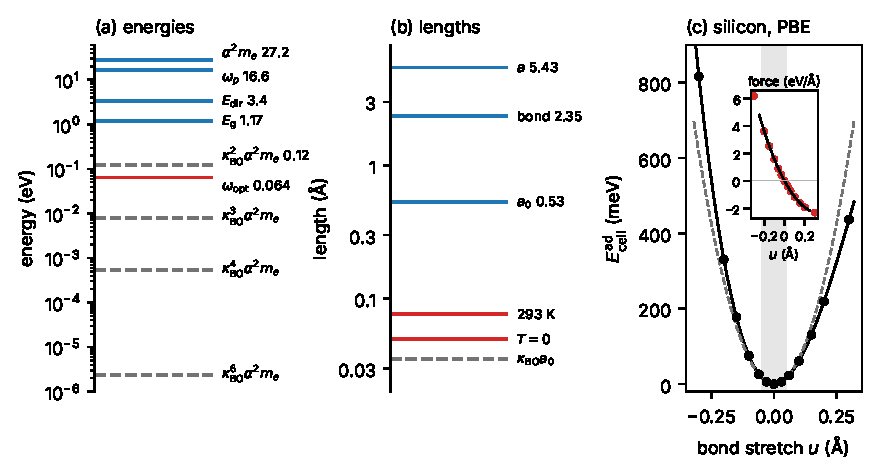
\includegraphics[width=\linewidth]{figures/ch05/fig5_1.pdf}
  \caption{Scales of electrons and nuclei in silicon. (a) Energies on a logarithmic axis, in eV. Electronic (blue): the atomic unit $\alpha^2m_e = \SI{27.2}{eV}$, the valence plasma energy $\omega_p = \SI{16.6}{eV}$, the direct gap $E_{\mathrm{dir}} = \SI{3.4}{eV}$ and the indirect gap $\Eg = \SI{1.17}{eV}$. Nuclear (red): the measured zone-center optical phonon, \SI{64.1}{meV} (\SI{15.5}{THz}), the highest vibrational energy of the crystal. Gray dashed: the Born--Oppenheimer estimates $\kappa_{\mathrm{BO}}^n\alpha^2m_e$ for $n = 2$ (phonons), 3 (cubic anharmonicity), 4 (anharmonic level shifts) and 6 (nonadiabatic level shifts), with $\kappa_{\mathrm{BO}} = (m_e/M)^{1/4} = 0.0665$ for $^{28}$Si. (b) Lengths on a logarithmic axis, in \AA: the lattice constant $a$, the bond length $\sqrt3a/4$ and the Bohr radius $a_0$ (blue). Red: the root-mean-square displacement of an atom along one Cartesian axis, $\langle u_x^2\rangle^{1/2}$, at \SI{293}{K} from a lattice-dynamical fit to neutron data and at $T = 0$ from the PBE phonon density of states. The PBE density of states uses the settings of panel (c) on a $4^3$ grid of phonon wavevectors. Gray dashed: the estimate $\kappa_{\mathrm{BO}}a_0$. (c) Energy per two-atom cell in a PBE calculation with an SG15 norm-conserving pseudopotential, a \SI{50}{Ry} cutoff, an $8^3$ grid of crystal momenta and $a = \SI{5.431}{\angstrom}$. The circles are computed at displacements in which the two atoms move in opposite directions along $[111]$ and the $[111]$ bond changes its length by $u$. The curves are a sixth-degree polynomial fit (solid) and the harmonic term $\tfrac12\Phi_{\mathrm{opt}}u^2$, $\Phi_{\mathrm{opt}} = \SI{13.6}{eV.\angstrom^{-2}}$ (dashed), from a quartic fit over $|u| \le \SI{0.1}{\angstrom}$. Shaded: $|u| < \ell_{\mathrm{zp}} = (M_\kappa\omega_{\mathrm{opt}})^{-1/2} = \SI{0.048}{\angstrom}$, the zero-point length of the coordinate $u$. Inset: Hellmann--Feynman force on $u$ (circles) and $-\dd E/\dd u$ from the sixth-degree fit (line).}
  \label{fig:5-scales}
\end{figure}

\begin{workedexample}{The small parameter of silicon}\label{we:5-kappa}
For natural silicon, $M = \SI{26.16}{GeV}$ and $m_e/M = 1.953\times10^{-5}$, so that
\begin{equation*}
  \kappa_{\mathrm{BO}} = 0.0665 , \qquad \kappa_{\mathrm{BO}}^2 = 4.42\times10^{-3} , \qquad \kappa_{\mathrm{BO}}^3 = 2.94\times10^{-4} .
\end{equation*}
The estimates \cref{eq:5.1-scales} are $\kappa_{\mathrm{BO}}a_0 = \SI{0.0352}{\angstrom}$ for the zero-point amplitude and $\kappa_{\mathrm{BO}}^2\alpha^2m_e = \SI{0.120}{eV}$ for a phonon. We compare them with the crystal (\cref{fig:5-scales}).

\emph{Energies.} The highest phonon of silicon, the optical mode at \SI{64.1}{meV}, is $\omega_{\mathrm{opt}}/\alpha^2m_e = 2.36\times10^{-3} = 0.53\,\kappa_{\mathrm{BO}}^2$: the counting, measured on the atomic scale for which it was built, is right to a factor of two. Against the gap the counting does much worse. The ratio is $\omega_{\mathrm{opt}}/\Eg = 0.0548 = 12.4\,\kappa_{\mathrm{BO}}^2$, because the gap of silicon is 23 times smaller than $\alpha^2m_e$. By \cref{eq:5.1-mixing}, $\omega_{\mathrm{ph}}/\Eg$ is the ratio that controls the mixing of excited electronic states into the ground state, so the adiabatic approximation in silicon is an order of magnitude less safe than the mass ratio alone suggests. It is still safe: the gap is eighteen phonon energies away. A semiconductor whose gap approaches the phonon energies, however, or a metal, is a different matter (\cref{sec:6.3}).

\emph{Lengths.} The zero-point amplitude of one Cartesian component is $\langle u_x^2\rangle^{1/2} = \SI{0.050}{\angstrom}$ in the PBE calculation of \cref{fig:5-scales}, 1.4 times $\kappa_{\mathrm{BO}}a_0$. At \SI{293}{K}, where thermal phonons add to the zero-point motion, a lattice-dynamical fit to neutron data gives \SI{0.0771}{\angstrom}, from $\langle u_x^2\rangle = \SI{0.005941}{\angstrom^2}$~\cite{flensburg1999lattice}, and the PBE calculation yields \SI{0.081}{\angstrom}, \SI{5}{\percent} more. This agreement suggests a similar accuracy for the zero-point value of the PBE calculation. Measured against the lattice constant, the zero-point amplitude is $\langle u_x^2\rangle^{1/2}/a = 0.0091$, seven times smaller than $\kappa_{\mathrm{BO}}$ itself. The reason for the factor of seven is the unit of length: the counting compares the amplitude with $a_0$, and the lattice constant of silicon is $10.3\,a_0$. As a fraction of the bond length, $4.4\,a_0$, the amplitude is 0.021.

\emph{Anharmonicity.} The fit of \cref{fig:5-scales}(c) has the cubic coefficient $\Phi^{(3)}_{\mathrm{opt}} = \SI{-41.5}{eV.\angstrom^{-3}}$. At $u = \ell_{\mathrm{zp}} = \SI{0.048}{\angstrom}$ the ratio of the cubic to the harmonic term of the energy is $|\Phi^{(3)}_{\mathrm{opt}}|\ell_{\mathrm{zp}}/3\Phi_{\mathrm{opt}} = 0.049$, against the estimate $\kappa_{\mathrm{BO}} = 0.067$.

\emph{Nonadiabatic shifts.} Their relative size is $\kappa_{\mathrm{BO}}^4 = m_e/M = 2\times10^{-5}$, about \SI{1}{\micro eV} on the optical phonon. A shift of \SI{1}{\micro eV} is far below the anharmonic effects and below any resolution that matters for detection.

The powers of $\kappa_{\mathrm{BO}}$ order the effects correctly, with coefficients between one half and two when the comparison is made in atomic units. The coefficients become large when a ratio is taken to a scale of the crystal itself, such as the gap or the lattice constant, and a calculation should quote ratios to these scales of the crystal.
\end{workedexample}

\section{The harmonic crystal}\label{sec:5.2}

Neutron scattering finds that the vibrations of silicon fill a band from zero up to \SI{64.1}{meV}, organized in six branches over the Brillouin zone. Three of them start at zero energy at the zone center and rise linearly, with slopes between 4.7 and \SI{9.4}{km.s^{-1}}: these are sound waves. Three start at the optical frequency and stay near it. The density of vibrational states piles up in sharp peaks, near \SI{17}{meV}, where the sound waves stop rising, and near \SI{60}{meV}, and a dark-matter particle that deposits energy in single phonons sees these peaks directly in its spectrum. All of this follows from the shape of the energy surface $E^{\mathrm{ad}}(u)$ of \cref{sec:5.1} near its minimum.

\subsection{Force constants and the dynamical matrix}

The displacement of the nucleus $\kappa$ in the cell $\vect{R}$ from its equilibrium site is $\vect{u}_{\vect{R}\kappa}$ (\cref{eq:5.1-X}), and the crystal has $n_{\mathrm{at}}$ nuclei per cell, two for silicon (\cref{sec:3.1}). Expanded about its minimum, the energy surface reads
\begin{equation}
  \begin{gathered}
  E^{\mathrm{ad}}(u) = E^{\mathrm{ad}}(0) + \frac12\sum_{\vect{R}\kappa\alpha}\sum_{\vect{R}'\kappa'\beta}\Phi^{(2),\alpha\beta}_{\kappa\kappa'}(\vect{R},\vect{R}')\,u^\alpha_{\vect{R}\kappa}u^\beta_{\vect{R}'\kappa'} + O(u^3) ,
  \\
  \Phi^{(2),\alpha\beta}_{\kappa\kappa'}(\vect{R},\vect{R}') = \frac{\partial^2E^{\mathrm{ad}}}{\partial u^\alpha_{\vect{R}\kappa}\,\partial u^\beta_{\vect{R}'\kappa'}}\bigg|_{u=0} ,
  \end{gathered}
  \label{eq:5.2-expand}
\end{equation}
with Cartesian indices $\alpha, \beta$. The linear term is absent, since every force vanishes at equilibrium. The coefficients $\Phi^{(2)}$ are the \emph{force constants}: $-\Phi^{(2),\alpha\beta}_{\kappa\kappa'}(\vect{R},\vect{R}')\,u^\beta_{\vect{R}'\kappa'}$ is the force along $\alpha$ on the nucleus $(\vect{R},\kappa)$ when the nucleus $(\vect{R}',\kappa')$ alone is displaced. As second derivatives they are symmetric under interchange of the two nuclei (the pair symmetry), $\Phi^{(2),\alpha\beta}_{\kappa\kappa'}(\vect{R},\vect{R}') = \Phi^{(2),\beta\alpha}_{\kappa'\kappa}(\vect{R}',\vect{R})$, and real. A lattice translation moves every nucleus to an equivalent site and leaves the surface unchanged. As a result the force constants depend on the two cells only through their separation, $\Phi^{(2)}_{\kappa\kappa'}(\vect{R},\vect{R}') = \Phi^{(2)}_{\kappa\kappa'}(\vect{0},\vect{R}'-\vect{R})$. Dropping the terms beyond second order is the \emph{harmonic approximation}. By the counting of \cref{sec:5.1}, the cubic term is smaller than the quadratic one by a factor $\sim\kappa_{\mathrm{BO}}$ at the zero-point amplitude, about \SI{5}{\percent} in silicon (\cref{we:5-kappa}), and we return to it in \cref{sec:5.7}.

The nuclei move in this quadratic potential. We treat their motion classically here. For a Hamiltonian quadratic in the coordinates and momenta, the Heisenberg equations of motion of the displacement operators are the same linear equations as the classical ones, so the normal modes we find are also those of the quantum problem; \cref{sec:5.3} quantizes them. Newton's law for each nucleus is
\begin{equation}
  M_\kappa\,\ddot u^\alpha_{\vect{R}\kappa} = -\frac{\partial E^{\mathrm{ad}}}{\partial u^\alpha_{\vect{R}\kappa}} = -\sum_{\vect{R}'\kappa'\beta}\Phi^{(2),\alpha\beta}_{\kappa\kappa'}(\vect{R},\vect{R}')\,u^\beta_{\vect{R}'\kappa'} ,
  \label{eq:5.2-eom}
\end{equation}
$3n_{\mathrm{at}}N$ coupled linear equations for a crystal of $N$ cells. Two steps reduce them to a small matrix problem: the mass weighting that works for any set of coupled oscillators, and the translation symmetry of the crystal. For a set of coordinates $x_i$ with masses $m_i$ and potential $\tfrac12\sum_{ij}K_{ij}x_ix_j$, the mass-weighted coordinates $y_i = \sqrt{m_i}\,x_i$ obey $\ddot y_i = -\sum_j(K_{ij}/\sqrt{m_im_j})\,y_j$. The matrix on the right is real and symmetric, so it has real eigenvalues $\omega^2$ and orthonormal eigenvectors, and each eigenvector oscillates on its own as $\ee^{-\ii\omega t}$: a normal mode. The crystal is such a system, with one more property. Its matrix is invariant under lattice translations, and a translation-invariant matrix is diagonalized by plane waves in the cell index. We therefore try
\begin{equation}
  u^\alpha_{\vect{R}\kappa}(t) = \frac{1}{\sqrt{M_\kappa}}\,e^\alpha_\kappa\,\ee^{\ii(\vect{Q}\cdot\vect{R} - \omega t)} ,
  \label{eq:5.2-ansatz}
\end{equation}
with a wavevector $\vect{Q}$ and $3n_{\mathrm{at}}$ amplitudes $e^\alpha_\kappa$ to be found. The physical displacement is the real part, or the sum of the solutions at $\vect{Q}$ and $-\vect{Q}$. Inserting \cref{eq:5.2-ansatz} into \cref{eq:5.2-eom}, dividing by $\sqrt{M_\kappa}\,\ee^{\ii(\vect{Q}\cdot\vect{R} - \omega t)}$ and writing $\vect{R}' = \vect{R} + \vect{R}''$, the sum over $\vect{R}''$ no longer depends on $\vect{R}$. What is left is an eigenvalue problem in the $3n_{\mathrm{at}}$ amplitudes,
\begin{equation}
  \sum_{\kappa'\beta}D^{\mathrm{dyn},\alpha\beta}_{\kappa\kappa'}(\vect{Q})\,e^\beta_{\kappa'\nu}(\vect{Q}) = \omega_{\vect{Q}\nu}^2\,e^\alpha_{\kappa\nu}(\vect{Q}) ,
  \qquad
  D^{\mathrm{dyn},\alpha\beta}_{\kappa\kappa'}(\vect{Q}) = \frac{1}{\sqrt{M_\kappa M_{\kappa'}}}\sum_{\vect{R}}\Phi^{(2),\alpha\beta}_{\kappa\kappa'}(\vect{0},\vect{R})\,\ee^{\ii\vect{Q}\cdot\vect{R}} ,
  \label{eq:5.2-Ddyn}
\end{equation}
the \emph{dynamical matrix} $D^{\mathrm{dyn}}(\vect{Q})$, the Fourier transform of the mass-weighted force constants~\cite{born1954dynamical}, \cite[Chaps.~22 and~23]{ashcroft1976solid}, \cite[Eq.~(14)]{giustino2017electron}; it is \cref{eq:A.6-Ddyn}. Its eigenvalues are labeled by the \emph{branch} index $\nu = 1,\dots,3n_{\mathrm{at}}$, and its eigenvectors $\vect{e}_{\kappa\nu}(\vect{Q})$, with one three-vector for each nucleus of the cell, are the \emph{polarization vectors}. The translation symmetry has turned $3n_{\mathrm{at}}N$ equations into $N$ independent problems of size $3n_{\mathrm{at}}$, one for each $\vect{Q}$: six by six for silicon. The phase in \cref{eq:5.2-Ddyn} contains the cell vector $\vect{R}$ and not the position $\vect{R} + \vect{\tau}_\kappa$ of the nucleus. Some codes and texts use the full position; the two choices differ by the phase $\ee^{\ii\vect{Q}\cdot\vect{\tau}_\kappa}$ on each component of $\vect{e}_{\kappa\nu}(\vect{Q})$ and give the same frequencies.

The properties of $D^{\mathrm{dyn}}$ follow from those of $\Phi^{(2)}$. By the pair symmetry of $\Phi^{(2)}$ and translation invariance, $\Phi^{(2),\beta\alpha}_{\kappa'\kappa}(\vect{0},\vect{R}) = \Phi^{(2),\alpha\beta}_{\kappa\kappa'}(\vect{0},-\vect{R})$, and replacing $\vect{R}$ by $-\vect{R}$ in the sum shows that $D^{\mathrm{dyn}}(\vect{Q})$ is Hermitian. Its eigenvalues $\omega_{\vect{Q}\nu}^2$ are therefore real and its eigenvectors orthonormal and complete,
\begin{equation}
  \sum_{\kappa\alpha}e^{\alpha}_{\kappa\nu}(\vect{Q})^*\,e^{\alpha}_{\kappa\nu'}(\vect{Q}) = \delta_{\nu\nu'} , \qquad
  \sum_\nu e^\alpha_{\kappa\nu}(\vect{Q})\,e^\beta_{\kappa'\nu}(\vect{Q})^* = \delta_{\kappa\kappa'}\delta_{\alpha\beta} ,
  \label{eq:5.2-ortho}
\end{equation}
which contains the normalization $\sum_\kappa|\vect{e}_{\kappa\nu}(\vect{Q})|^2 = 1$ of \cref{eq:A.6-e}. At a minimum of $E^{\mathrm{ad}}$ the quadratic form \cref{eq:5.2-expand} is non-negative for every displacement, and so is $D^{\mathrm{dyn}}(\vect{Q})$ for every $\vect{Q}$; every $\omega_{\vect{Q}\nu}^2$ is then non-negative and $\omega_{\vect{Q}\nu}$ real. A computed $\omega_{\vect{Q}\nu}^2 < 0$, usually printed as an imaginary frequency, signals that the structure is not at a minimum, or that the calculation is not converged. Since $\ee^{\ii\vect{G}\cdot\vect{R}} = 1$, $D^{\mathrm{dyn}}(\vect{Q} + \vect{G}) = D^{\mathrm{dyn}}(\vect{Q})$, and $\vect{Q}$ can be taken in the first Brillouin zone: a displacement wave of wavevector $\vect{Q} + \vect{G}$ moves the nuclei exactly as one of wavevector $\vect{Q}$, because the nuclei sit only at the lattice sites. Under Born--von Karman conditions there are $N$ allowed $\vect{Q}$ in the zone (\cref{sec:3.1}), and the crystal has $3n_{\mathrm{at}}N$ modes, one for each degree of freedom. Finally, since the force constants are real, $D^{\mathrm{dyn}}(-\vect{Q}) = D^{\mathrm{dyn}}(\vect{Q})^*$. As a result $\omega_{-\vect{Q}\nu} = \omega_{\vect{Q}\nu}$, and the phases can be chosen so that $\vect{e}_{\kappa\nu}(-\vect{Q}) = \vect{e}_{\kappa\nu}(\vect{Q})^*$, the convention of \cref{eq:A.6-e}.

A quick estimate fixes the scale. The force constant between neighbors is $\Phi^{(2)} \sim \alpha^2m_e/a_0^2 \sim \SI{100}{eV.\angstrom^{-2}}$ by the counting of \cref{sec:5.1}, and the frequencies are $\omega \sim (\Phi^{(2)}/M_\kappa)^{1/2}$. For silicon the zone-center optical mode of \cref{fig:5-scales} has $\Phi_{\mathrm{opt}} = \SI{13.6}{eV.\angstrom^{-2}}$ and $\omega = \SI{63.7}{meV}$ in the same calculation: the estimate is high by a factor of seven in the force constant, and the frequencies are tens of meV.

The force constants are computed, not fitted. Each $\Phi^{(2)}$ is a second derivative of the Kohn--Sham total energy, and density-functional perturbation theory evaluates the whole matrix $D^{\mathrm{dyn}}(\vect{Q})$ at a given $\vect{Q}$ from the linear response of the electrons to a displacement wave. A calculation computes it on a coarse uniform grid of $\vect{Q}$, transforms back to real-space force constants, and evaluates \cref{eq:5.2-Ddyn} at any $\vect{Q}$ from them. The phonons of silicon shown below come from such a calculation.

\begin{workedexample}{The diatomic chain}\label{we:5-chain}
The simplest crystal with both kinds of branch is a line of nuclei of masses $M_1$ and $M_2$, alternating, with period $a_{\mathrm{c}}$ and a spring of stiffness $K$ between neighbors. The nucleus 1 of cell $R$ is tied to the nucleus 2 of the same cell and to the nucleus 2 of the cell $R - a_{\mathrm{c}}$, and the energy is $\tfrac12K\sum_R[(u_{R2} - u_{R1})^2 + (u_{R+a_{\mathrm{c}},1} - u_{R2})^2]$. Differentiating twice, the nonzero force constants from the cell at the origin are $\Phi^{(2)}_{11}(0,0) = \Phi^{(2)}_{22}(0,0) = 2K$, $\Phi^{(2)}_{12}(0,0) = \Phi^{(2)}_{12}(0,-a_{\mathrm{c}}) = -K$ and $\Phi^{(2)}_{21}(0,0) = \Phi^{(2)}_{21}(0,a_{\mathrm{c}}) = -K$. By \cref{eq:5.2-Ddyn},
\begin{equation*}
  D^{\mathrm{dyn}}(Q) = \begin{pmatrix} 2K/M_1 & -K(1 + \ee^{-\ii Qa_{\mathrm{c}}})/\sqrt{M_1M_2} \\ -K(1 + \ee^{\ii Qa_{\mathrm{c}}})/\sqrt{M_1M_2} & 2K/M_2 \end{pmatrix} ,
\end{equation*}
which is Hermitian, as it must be. With $|1 + \ee^{\ii Qa_{\mathrm{c}}}|^2 = 4\cos^2(Qa_{\mathrm{c}}/2)$, the eigenvalues solve $\omega^4 - 2K(M_1^{-1} + M_2^{-1})\,\omega^2 + 4K^2\sin^2(Qa_{\mathrm{c}}/2)/(M_1M_2) = 0$:
\begin{equation*}
  \omega_{Q\pm}^2 = K\Bigl(\frac{1}{M_1} + \frac{1}{M_2}\Bigr) \pm K\Bigl[\Bigl(\frac{1}{M_1} + \frac{1}{M_2}\Bigr)^2 - \frac{4\sin^2(Qa_{\mathrm{c}}/2)}{M_1M_2}\Bigr]^{1/2} .
\end{equation*}
The lower branch vanishes at $Q = 0$. For $Qa_{\mathrm{c}} \ll 1$, expanding the square root to first order in its small term, $\omega_{Q-}^2 = 2K\sin^2(Qa_{\mathrm{c}}/2)/(M_1 + M_2) \simeq KQ^2a_{\mathrm{c}}^2/[2(M_1 + M_2)]$: the frequency is linear in $Q$, a sound wave with speed $c = a_{\mathrm{c}}[K/2(M_1 + M_2)]^{1/2}$, in which the chain moves as a medium of mass $M_1 + M_2$ per length $a_{\mathrm{c}}$. Its eigenvector at $Q = 0$ is $\vect{e} \propto (\sqrt{M_1}, \sqrt{M_2})$, so that by \cref{eq:5.2-ansatz} both nuclei move by the same amount: a rigid translation. This is the \emph{acoustic} branch. The upper branch starts at $\omega_{0+}^2 = 2K/\mu_{\mathrm{red}}$, with $\mu_{\mathrm{red}} = M_1M_2/(M_1 + M_2)$, and its eigenvector at $Q = 0$ is $\vect{e} \propto (\sqrt{M_2}, -\sqrt{M_1})$: the two nuclei move against each other, $u_1/u_2 = -M_2/M_1$, and the center of mass of each cell stays at rest. This is the \emph{optical} branch, so named because, when the two nuclei carry opposite charges, its oscillating dipole couples to light (\cref{sec:5.5}). At the zone boundary, $Q = \pi/a_{\mathrm{c}}$, the off-diagonal elements vanish. Each mode then moves one species only, with $\omega^2 = 2K/M_1$ and $2K/M_2$, and between them lies a gap in which no wave propagates.

For equal masses the gap closes. Then $\omega_{Q\pm} = (2K/M)^{1/2}[1 \pm \cos(Qa_{\mathrm{c}}/2)]^{1/2}$, which is the single branch $\omega = 2(K/M)^{1/2}|\sin(Q'a_{\mathrm{c}}/4)|$ of a chain of identical nuclei with period $a_{\mathrm{c}}/2$, with $Q' = Q$ on the acoustic branch and $Q' = 2\pi/a_{\mathrm{c}} - Q$ on the optical one. The doubled cell has folded the zone in half, and the optical branch is the far half of the acoustic one. Silicon contains exactly this chain. For a wave along $[100]$ with longitudinal polarization, every atomic plane perpendicular to $[100]$ moves rigidly, and the planes, \SI{1.358}{\angstrom} ($a/4$) apart, alternate between the two sublattices of the diamond structure. The two kinds of plane are related by a translation by $a/4$ combined with a rotation by \ang{90} about $[100]$, and the rotation does not affect a longitudinal motion. The planes therefore act as identical masses, and the longitudinal branches along $[100]$ form a folded chain with $a_{\mathrm{c}} = a/2$. Its zone boundary is $Q = 2\pi/a$, the point X. In the folded chain the longitudinal acoustic and optical branches must meet there, whatever the range of the interplanar forces, and in silicon they do, at \SI{12.32}{THz}~\cite{nilsson1972study}.
\end{workedexample}

\subsection{The acoustic sum rule}

The acoustic branch of the chain vanished at $Q = 0$ because a rigid translation costs no energy. This holds for every crystal. Displacing all nuclei by the same vector $\vect{d}$ leaves the energy unchanged at any configuration, $E^{\mathrm{ad}}(u + d) = E^{\mathrm{ad}}(u)$, where $u + d$ means $\vect{u}_{\vect{R}\kappa} + \vect{d}$ for every nucleus. Differentiating with respect to $u^\alpha_{\vect{R}\kappa}$ and to $d^\beta$, and setting $u = d = 0$, yields $\sum_{\vect{R}'\kappa'}\partial^2E^{\mathrm{ad}}/\partial u^\alpha_{\vect{R}\kappa}\partial u^\beta_{\vect{R}'\kappa'} = 0$, that is
\begin{equation}
  \sum_{\vect{R}\kappa'}\Phi^{(2),\alpha\beta}_{\kappa\kappa'}(\vect{0},\vect{R}) = 0 \qquad \text{for every } \kappa, \alpha, \beta .
  \label{eq:5.2-asr}
\end{equation}
This is the \emph{acoustic sum rule}: the force on a nucleus when all others, and the nucleus itself, are moved together vanishes. Its consequence for the dynamical matrix follows at once. At $\vect{Q} = 0$, the vector $e^\beta_{\kappa'} = (M_{\kappa'}/M_{\mathrm{cell}})^{1/2}\hat e^\beta$, with $M_{\mathrm{cell}} = \sum_\kappa M_\kappa$ and any unit vector $\hat{\vect{e}}$, gives $\sum_{\kappa'\beta}D^{\mathrm{dyn},\alpha\beta}_{\kappa\kappa'}(\vect{0})\,e^\beta_{\kappa'} = (M_\kappa M_{\mathrm{cell}})^{-1/2}\sum_\beta\bigl[\sum_{\vect{R}\kappa'}\Phi^{(2),\alpha\beta}_{\kappa\kappa'}(\vect{0},\vect{R})\bigr]\hat e^\beta = 0$. Three independent choices of $\hat{\vect{e}}$ give three modes of zero frequency at the zone center, the \emph{acoustic} branches, in which all nuclei move together. These are the polarization vectors of \cref{app:A.6}, $\vect{e}_{\kappa\nu} = (M_\kappa/M_{\mathrm{cell}})^{1/2}\hat{\vect{e}}_\nu$. The other $3n_{\mathrm{at}} - 3$ branches, three in silicon, are the \emph{optical} branches, finite at $\vect{Q} = 0$. In them the nuclei of a cell move against each other with their center of mass at rest: orthogonality to the three acoustic vectors in \cref{eq:5.2-ortho} is $\sum_\kappa\sqrt{M_\kappa}\,\vect{e}_{\kappa\nu}(\vect{0}) = 0$, and the displacement $\vect{e}_{\kappa\nu}/\sqrt{M_\kappa}$ of \cref{eq:5.2-ansatz} then has $\sum_\kappa M_\kappa\,\vect{u}_\kappa = 0$. In field-theory language the acoustic phonons are the Goldstone modes of the translation symmetry that the crystal breaks~\cite[p.~69]{lin2019tasi}. A uniform translation is a different ground state at the same energy, and a translation that varies slowly in space costs an energy that vanishes as its wavelength grows.

A computed set of force constants violates \cref{eq:5.2-asr} slightly, chiefly because the exchange--correlation potential is evaluated on a real-space grid that is not invariant under arbitrary translations. The acoustic frequencies at $\mathrm{\Gamma}$ then come out small but nonzero, \SI{0.16}{THz} in the calculation of \cref{fig:5-si}, and codes restore the rule by correcting the on-site constants.

\subsection{Sound speeds}

Near $\vect{Q} = 0$ the acoustic frequencies rise from zero, and we want the rate at which they do. Expanding the exponential in \cref{eq:5.2-Ddyn} in powers of $\vect{Q}$,
\begin{equation}
  \begin{gathered}
  D^{\mathrm{dyn}}(\vect{Q}) = D_0 + D_1(\vect{Q}) + D_2(\vect{Q}) + O(Q^3) , \\
  D^{\alpha\beta}_{n,\kappa\kappa'}(\vect{Q}) = \frac{1}{\sqrt{M_\kappa M_{\kappa'}}}\sum_{\vect{R}}\Phi^{(2),\alpha\beta}_{\kappa\kappa'}(\vect{0},\vect{R})\,\frac{(\ii\vect{Q}\cdot\vect{R})^n}{n!} ,
  \end{gathered}
  \label{eq:5.2-Dexp}
\end{equation}
and treating $D_1$ and $D_2$ as perturbations of $D_0 = D^{\mathrm{dyn}}(\vect{0})$, whose acoustic eigenvalue is triply degenerate at zero, leads to $\omega^2$ as an expansion in $Q$. The acoustic frequencies are the eigenvalues of a $3\times3$ matrix in the space of the three acoustic vectors $\vect{a}_{\hat{\vect{e}}}$, with components $(M_\kappa/M_{\mathrm{cell}})^{1/2}\hat{\vect{e}}$.

The first-order term would make $\omega^2$ linear in $Q$, and $\omega \propto Q^{1/2}$, which no crystal shows. Rotational invariance makes it vanish. Its matrix elements are
\begin{equation*}
  \vect{a}_{\hat{\vect{e}}}^\dagger D_1\,\vect{a}_{\hat{\vect{e}}'} = \frac{\ii Q_\gamma}{M_{\mathrm{cell}}}\,\hat e^\alpha\hat e'^\beta\,T^{\alpha\beta\gamma} , \qquad
  T^{\alpha\beta\gamma} = \sum_{\kappa\kappa'\vect{R}}\Phi^{(2),\alpha\beta}_{\kappa\kappa'}(\vect{0},\vect{R})\,R^\gamma ,
\end{equation*}
with summation over repeated Cartesian indices. Two properties of $T$ force it to zero. The first follows from the pair symmetry of $\Phi^{(2)}$. Writing $\Phi^{(2),\beta\alpha}_{\kappa\kappa'}(\vect{0},\vect{R}) = \Phi^{(2),\alpha\beta}_{\kappa'\kappa}(\vect{0},-\vect{R})$ and relabeling $\kappa \leftrightarrow \kappa'$ and $\vect{R} \to -\vect{R}$ in the sum shows $T^{\beta\alpha\gamma} = -T^{\alpha\beta\gamma}$. The second follows from rotations. A rigid infinitesimal rotation by the angle vector $\vect{\theta}$ moves every nucleus, at whatever position $\vect{X}_I$ it has, by $\vect{\theta}\times\vect{X}_I$ and leaves the energy unchanged. (For a crystal under Born--von Karman conditions a rotation is not a symmetry, but the force constants are those of a large free crystal, for which it is.) Hence $\sum_I\nabla_IE^{\mathrm{ad}}\cdot(\vect{\theta}\times\vect{X}_I) = 0$ at every configuration: the total torque vanishes. Differentiating this identity with respect to the displacement of one nucleus and evaluating at equilibrium, where the forces vanish, leaves $\sum_I\Phi^{(2)}_{JI}\,(\vect{\theta}\times\vect{X}_I) = 0$ for every $J$ and every $\vect{\theta}$. In components, $\sum_{\vect{R}\kappa'}\Phi^{(2),\alpha\beta}_{\kappa\kappa'}(\vect{0},\vect{R})\,X^\gamma_{\vect{R}\kappa'}$ is symmetric in $\beta\gamma$, with $\vect{X}_{\vect{R}\kappa'} = \vect{R} + \vect{\tau}_{\kappa'}$. Summed over $\kappa$, it is $T^{\alpha\beta\gamma}$ plus a term $\sum_{\kappa\kappa'}[\sum_{\vect{R}}\Phi^{(2)}_{\kappa\kappa'}(\vect{0},\vect{R})]\tau^\gamma_{\kappa'}$, which vanishes because the sum rule \cref{eq:5.2-asr} also holds with the roles of $\kappa$ and $\kappa'$ exchanged (by the same pair symmetry). So $T^{\alpha\beta\gamma}$ is symmetric in $\beta\gamma$ and antisymmetric in $\alpha\beta$, and a tensor with both properties is zero. Alternating the two properties six times returns to the start with a minus sign~\cite[Chap.~V]{born1954dynamical}:
\begin{equation*}
  T^{\alpha\beta\gamma} = -T^{\beta\alpha\gamma} = -T^{\beta\gamma\alpha} = T^{\gamma\beta\alpha} = T^{\gamma\alpha\beta} = -T^{\alpha\gamma\beta} = -T^{\alpha\beta\gamma} = 0 .
\end{equation*}

At second order two terms contribute. One is the expectation value of $D_2$ in the acoustic space. The other is $D_1$ taken twice, through the optical modes: $D_1$ does connect an acoustic vector to an optical one at $\vect{Q} = 0$, with frequency $\omega_{\mathrm{o}}$, and second-order perturbation theory adds $-|\vect{o}^\dagger D_1\vect{a}_{\hat{\vect{e}}}|^2/\omega_{\mathrm{o}}^2$. Both are quadratic in $\vect{Q}$, so
\begin{equation}
  \omega_{\vect{Q}\nu}^2 = \Lambda^{\mathrm{ac}}_\nu(\hat{\vect{Q}})\,Q^2 + O(Q^3), \qquad
  \omega_{\vect{Q}\nu} = c_\nu(\hat{\vect{Q}})\,Q , \qquad c_\nu(\hat{\vect{Q}}) = \Lambda^{\mathrm{ac}}_\nu(\hat{\vect{Q}})^{1/2} ,
  \label{eq:5.2-sound}
\end{equation}
where $\Lambda^{\mathrm{ac}}_\nu(\hat{\vect{Q}})$ are the three eigenvalues of the $3\times3$ matrix
\begin{equation*}
  \Lambda^{\mathrm{ac},\alpha\beta}(\hat{\vect{Q}})\,Q^2 = -\frac{1}{2M_{\mathrm{cell}}}\sum_{\kappa\kappa'\vect{R}}\Phi^{(2),\alpha\beta}_{\kappa\kappa'}(\vect{0},\vect{R})\,(\vect{Q}\cdot\vect{R})^2
  - \sum_{\mathrm{o}}\frac{(\vect{a}_\alpha^\dagger D_1\vect{o})(\vect{o}^\dagger D_1\vect{a}_\beta)}{\omega_{\mathrm{o}}^2} ,
\end{equation*}
with $\vect{a}_\alpha$ the acoustic vector polarized along the axis $\alpha$ and the sum over the optical modes at $\vect{Q} = 0$. The frequency of an acoustic mode is linear in $Q$, with a sound speed $c_\nu(\hat{\vect{Q}})$ that depends on the direction of propagation and on the branch, and the polarizations $\hat{\vect{e}}_\nu(\hat{\vect{Q}})$ are the eigenvectors of $\Lambda^{\mathrm{ac}}$. The first term is the stiffness of the crystal when every nucleus follows the long wave rigidly, the sum of the springs weighted by the squared lengths over which they are stretched. The second lowers it. In a crystal with more than one nucleus per cell, a strain pushes the sublattices against each other, and the optical coordinate relaxes in the long wave; this internal relaxation, which in the diamond structure reduces the shear stiffness, is what the second term describes~\cite[Chap.~V]{born1954dynamical}. In silicon the first-order coupling $D_1$ from acoustic to optical vectors vanishes for the longitudinal wave along $[100]$, in which the planes of \cref{we:5-chain} move as identical masses and the two sublattices are not pushed against each other, but not for shear waves.

Since $\Lambda^{\mathrm{ac}}$ describes a long wave, it is a property of the crystal as an elastic continuum. \Cref{app:C.18} derives the equation of motion of such a continuum, the Christoffel equation, with the elastic constants $C_{ijkl}$ and the mass density $\rho_T$, and \cref{eq:5.2-sound} is the same equation: $\rho_T\Lambda^{\mathrm{ac}}$, with $\rho_T = M_{\mathrm{cell}}/\Omega$, is the Christoffel matrix of the relaxed elastic constants. For a cubic crystal along $[100]$ this reads $\rho_Tc_{\mathrm{LA}}^2 = C_{11}$ and $\rho_Tc_{\mathrm{TA}}^2 = C_{44}$ for the two degenerate transverse branches. The sound speeds of the dark-matter kinematics of \cref{sec:1.3} are these slopes, and the acoustic edge $m^{\mathrm{ac}}_{\mathrm{min}}$ of \cref{sec:9.2} uses them. The longitudinal speed is the largest, since compressing a medium costs more than shearing it. The scale is a vibrational frequency $(\Phi^{(2)}/M_\kappa)^{1/2}$ times a distance of the order of the spacing between atomic planes: for silicon, the optical frequency times $a/4$ is \SI{13}{km.s^{-1}}, against measured speeds of 4.7 to \SI{9.4}{km.s^{-1}}. Note that $c/v_{\mathrm{max}} \sim 10^{-2}$: sound is two orders of magnitude slower than the fastest dark matter, which is why an acoustic phonon takes only a small fraction of the kinetic energy (\cref{sec:1.3}).

\subsection{The phonons of silicon}

\Cref{fig:5-si}(a) shows the six branches of silicon along the three lines of the zone on which they were measured: from $\mathrm{\Gamma}$ to X along $[100]$, from X to $\mathrm{\Gamma}$ along $[110]$ through K, and from $\mathrm{\Gamma}$ to L along $[111]$. On these lines the symmetry of the crystal makes every polarization either parallel or perpendicular to $\vect{Q}$, and the branches are named accordingly: longitudinal and transverse acoustic (LA, TA), longitudinal and transverse optical (LO, TO). In a general direction the polarizations mix, and the names refer to the branch that is mostly longitudinal or mostly transverse. Along $[100]$ and $[111]$ the two transverse branches of each kind are degenerate by the symmetry of these axes; along $[110]$ they split.

The measured frequencies at the high-symmetry points come from inelastic neutron scattering at room temperature~\cite{dolling1963inelastic,nilsson1972study}. At $\mathrm{\Gamma}$ the three optical modes are degenerate, at \SI{15.5}{THz}, or \SI{64.1}{meV}. In a polar crystal the longitudinal one would be pushed up by the electric field it creates, the LO--TO splitting of \cref{sec:5.5}; silicon has no Born charges and no splitting. At X the longitudinal acoustic and optical branches meet, at \SI{12.32}{THz} (\SI{50.95}{meV}), as the folded chain of \cref{we:5-chain} requires. Near the zone boundary the transverse acoustic branches bend over and become almost flat, at \SI{4.49}{THz} (\SI{18.6}{meV}) at X and \SI{3.43}{THz} (\SI{14.2}{meV}) at L. The reason is the covalent bond. Stretching a bond is stiff, while changing the angle between two bonds is soft, and a short-wavelength transverse wave mostly bends bonds. Finally, the optical branches are narrow. From \SI{15.5}{THz} at $\mathrm{\Gamma}$ they fall only to between 12.3 and \SI{14.7}{THz} at the zone boundary. The reason is that the motion of the two atoms of a cell against each other is controlled by the stiff bond between them and depends only weakly on what the neighboring cells do.

The lines in \cref{fig:5-si}(a) are a density-functional calculation with the PBE functional at the measured lattice constant, from force constants computed by density-functional perturbation theory (DFPT) on a $6^3$ grid of wavevectors. They follow the measurements closely. Of the eight measured frequencies at $\mathrm{\Gamma}$, X and L, six agree to within \SI{2}{\percent}, and the mean absolute difference over all eight is \SI{2.6}{\percent}. The zone-center optical mode comes out at \SI{15.40}{THz} (\SI{63.7}{meV}), \SI{0.6}{\percent} below the measured \SI{64.1}{meV} and the same as the frozen-phonon value of \cref{fig:5-scales}. The exceptions are the flat transverse acoustic modes, \SI{8}{\percent} soft: \num{4.13} against \SI{4.49}{THz} at X and \num{3.17} against \SI{3.43}{THz} at L. PBE generally puts the phonons of silicon and germanium below the measured ones, a consequence of its underbinding~\cite[Sect.~V]{haxhijaj2026lattice}; in this calculation the deficit is largest on the branches set by bond bending, the weakest force constant of the crystal. The calculation describes a static lattice, while the measurement was made at room temperature, where the frequencies are lower by thermal expansion and by anharmonic shifts; these effects, and the widths $\gamma_{\vect{Q}\nu}$ that the harmonic crystal lacks entirely, are the subject of \cref{sec:5.7}. A frequency also moves with the lattice constant at which it is computed, by an amount set by its Grüneisen parameter $\gamma^{\mathrm{G}}_{\vect{Q}\nu} = -\partial\ln\omega_{\vect{Q}\nu}/\partial\ln\Omega$. For most modes of silicon $\gamma^{\mathrm{G}}_{\vect{Q}\nu} > 0$, and the PBE lattice constant, \SI{0.85}{\percent} too large, would soften them; the flat transverse acoustic modes have $\gamma^{\mathrm{G}}_{\vect{Q}\nu} < 0$ and would stiffen.

\begin{figure}[tbp]
  \centering
  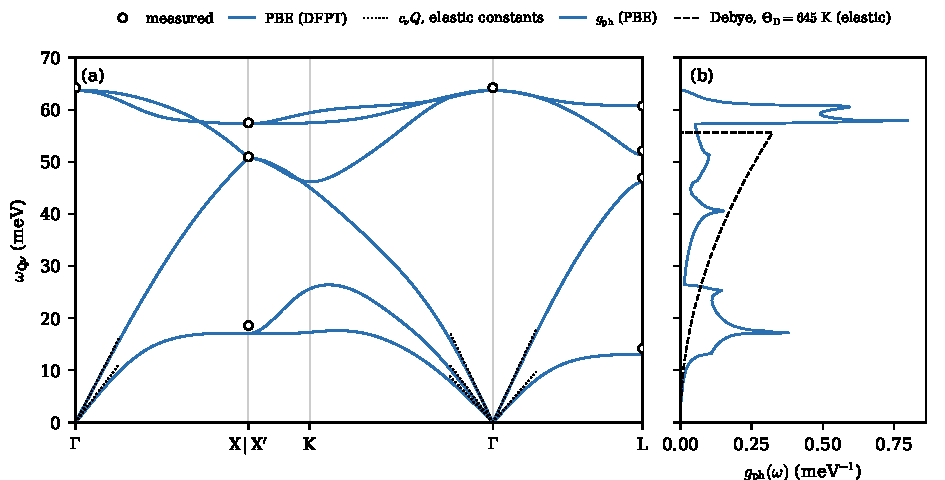
\includegraphics[width=\linewidth]{figures/ch05/fig5_2.pdf}
  \caption{Phonons of silicon. (a) Dispersion along $[100]$ from $\mathrm{\Gamma}$ to X, along $[110]$ from X$'$ $= (1,1,0)2\pi/a$, which is equivalent to X, through K to $\mathrm{\Gamma}$, and along $[111]$ from $\mathrm{\Gamma}$ to L. Lines: density-functional perturbation theory with the PBE functional, an SG15 norm-conserving pseudopotential, a \SI{60}{Ry} cutoff, a $12^3$ grid of crystal momenta, the measured lattice constant $a = \SI{5.431}{\angstrom}$ and the natural mass of silicon; force constants from a $6^3$ grid of wavevectors, with the acoustic sum rule imposed, interpolated to the path. Circles: frequencies measured by inelastic neutron scattering at room temperature at $\mathrm{\Gamma}$, X and L~\cite{dolling1963inelastic,nilsson1972study}, as tabulated in Ref.~\cite[Table~I]{savrasov1996linear}. Dotted: $\omega = c_\nu Q$ with the sound speeds of the measured elastic constants (\cref{we:5-debye}), drawn up to $Q = 0.25\,(2\pi/a)$. (b) Phonon density of states per two-atom cell, normalized to six modes, from the same force constants on a $48^3$ grid (tetrahedron integration), and the Debye model \cref{eq:5.2-gD} with $\bar c$ from the measured elastic constants, $\omega_{\mathrm{D}} = \SI{55.6}{meV}$, in the convention of one wavevector per atom. One THz corresponds to \SI{4.136}{meV}.}
  \label{fig:5-si}
\end{figure}

\subsection{The density of states}

For any quantity that sums over all phonons, such as a rate summed over final states or a thermal average, what matters is how many modes there are at each frequency. The phonon density of states per cell is
\begin{equation}
  g_{\mathrm{ph}}(\omega) = \frac1N\sum_{\vect{Q}\nu}\delta(\omega - \omega_{\vect{Q}\nu}) = \frac{\Omega}{(2\pi)^3}\sum_\nu\int_{\mathrm{BZ}}\dd^3Q\;\delta(\omega - \omega_{\vect{Q}\nu}) ,
  \qquad \int_0^\infty\dd\omega\,g_{\mathrm{ph}}(\omega) = 3n_{\mathrm{at}} ,
  \label{eq:5.2-dos}
\end{equation}
where the sum over the $N$ wavevectors of the zone became an integral with the density $\Vol/(2\pi)^3$ of \cref{sec:3.1}, $\Vol = N\Omega$. Its integral counts the $3n_{\mathrm{at}}$ modes per cell, six for silicon. A density of states per atom, normalized to three, is $g_{\mathrm{ph}}/n_{\mathrm{at}}$. In silicon, \cref{fig:5-si}(b), $g_{\mathrm{ph}}$ has a sharp peak at \SI{17}{meV} from the flat transverse acoustic branches near the zone boundary. Above it lies a structured region between 25 and \SI{52}{meV} from the longitudinal acoustic branch and the lower optical branches. The tallest peaks, at 58 and \SI{61}{meV}, come from the flat transverse optical branches. The peaks are where the branches are flat. Near a frequency at which $\nabla_{\vect{Q}}\omega_{\vect{Q}\nu}$ vanishes, many wavevectors share nearly the same frequency, and in three dimensions the density of states has a kink with an infinite slope there, a Van Hove singularity~\cite[Chap.~23]{ashcroft1976solid}. The large peak of the transverse acoustic branches is what makes silicon's low-energy phonons so numerous: a dark-matter particle that can deposit \SI{20}{meV} in single phonons finds a fifth of all modes of the crystal, \SI{22}{\percent} in the calculation, below that energy.

At low frequency only the acoustic branches contribute, with $\omega_{\vect{Q}\nu} = c_\nu(\hat{\vect{Q}})Q$. Writing $\dd^3Q = Q^2\dd Q\,\dd\hat{\vect{Q}}$ and integrating over $Q$ with $\int Q^2\dd Q\,\delta(\omega - c_\nu Q) = \omega^2/c_\nu^3$,
\begin{equation}
  g_{\mathrm{ph}}(\omega) \simeq \frac{\Omega\,\omega^2}{2\pi^2}\sum_\nu\bigl\langle c_\nu^{-3}\bigr\rangle , \qquad
  \bigl\langle c_\nu^{-3}\bigr\rangle = \int\frac{\dd\hat{\vect{Q}}}{4\pi}\,c_\nu(\hat{\vect{Q}})^{-3} ,
  \label{eq:5.2-dosac}
\end{equation}
an $\omega^2$ law with a coefficient fixed by the sound speeds alone, averaged over directions. It holds as long as the dispersion is linear, which in silicon means up to about \SI{7}{meV}, where the computed $g_{\mathrm{ph}}$ exceeds the $\omega^2$ law by \SI{10}{\percent}.

\subsection{The Debye model}

Debye's model extends \cref{eq:5.2-dosac} to the whole spectrum. It replaces the $3n_{\mathrm{at}}$ branches by three, all with the linear dispersion $\omega = \bar cQ$ of a single averaged speed $\bar c$. It also replaces the zone by a sphere of radius $Q_{\mathrm{D}}$ that holds one wavevector per atom, $n_{\mathrm{at}}N$ in all, so that the three branches carry all $3n_{\mathrm{at}}N$ degrees of freedom~\cite[Chap.~23]{ashcroft1976solid}. Counting with the density $\Vol/(2\pi)^3$, $(4\pi Q_{\mathrm{D}}^3/3)\,N\Omega/(2\pi)^3 = n_{\mathrm{at}}N$, so that
\begin{equation}
  Q_{\mathrm{D}} = \Bigl(\frac{6\pi^2n_{\mathrm{at}}}{\Omega}\Bigr)^{1/3} , \qquad
  \omega_{\mathrm{D}} = \bar c\,Q_{\mathrm{D}} , \qquad
  \Theta_{\mathrm{D}} = \omega_{\mathrm{D}} ,
  \label{eq:5.2-debye}
\end{equation}
with the Debye frequency $\omega_{\mathrm{D}}$ and the Debye temperature $\Theta_{\mathrm{D}}$, which in natural units are the same number. The density of states of the model follows from \cref{eq:5.2-dosac} with $c_\nu = \bar c$, cut off at $\omega_{\mathrm{D}}$:
\begin{equation}
  g_{\mathrm{D}}(\omega) = \frac{3\Omega\,\omega^2}{2\pi^2\bar c^3}\,\Theta(\omega_{\mathrm{D}} - \omega) = \frac{9n_{\mathrm{at}}\,\omega^2}{\omega_{\mathrm{D}}^3}\,\Theta(\omega_{\mathrm{D}} - \omega) ,
  \label{eq:5.2-gD}
\end{equation}
where the second form uses \cref{eq:5.2-debye}; its integral is $3n_{\mathrm{at}}$, as it must be. Matching the low-frequency limit \cref{eq:5.2-dosac} exactly fixes the speed,
\begin{equation}
  \frac{3}{\bar c^3} = \sum_\nu\bigl\langle c_\nu^{-3}\bigr\rangle .
  \label{eq:5.2-cbar}
\end{equation}
This is the definition we use. It makes the model exact wherever only long acoustic waves matter, as in the heat capacity at low temperature, which then follows Debye's $T^3$ law with this $\Theta_{\mathrm{D}}$, and in a dark-matter rate dominated by the lowest phonon energies. Since $c^{-3}$ is averaged, the slowest branches dominate $\bar c$. Note that the literature also uses a second convention. Some texts, particularly on phonon transport, put only the $N$ acoustic wavevectors in the sphere, one per cell, which lowers $Q_{\mathrm{D}}$ and $\Theta_{\mathrm{D}}$ by the factor $n_{\mathrm{at}}^{1/3}$, $2^{1/3} = 1.26$ for silicon, and treats the optical branches separately.

Above a few meV, however, the model is crude. It puts all modes below $\omega_{\mathrm{D}}$, and in silicon it misses both the peak of the flat transverse branches and the optical band at the top. Its strength is that one number fixes the low-energy spectrum, and any quantity that is an integral over $g_{\mathrm{ph}}$ weighted toward low frequencies, such as the mean-square displacement at room temperature (\cref{sec:5.3}) or the Debye--Waller exponent (\cref{sec:5.6}), comes out within tens of percent. \Cref{we:5-debye} carries this through for silicon.

\begin{workedexample}{Silicon sound speeds and Debye temperature}\label{we:5-debye}
The elastic constants of silicon at room temperature are $C_{11} = \SI{165.6}{GPa}$, $C_{12} = \SI{63.9}{GPa}$ and $C_{44} = \SI{79.5}{GPa}$, and its density is $\rho_T = \SI{2.33}{g.cm^{-3}}$~\cite[Table~I]{martinez2019measurements}. Along $[100]$, $\rho_Tc_{\mathrm{LA}}^2 = C_{11}$ and $\rho_Tc_{\mathrm{TA}}^2 = C_{44}$, so
\begin{gather*}
  c_{\mathrm{LA}} = \Bigl(\frac{\SI{165.6e9}{Pa}}{\SI{2330}{kg.m^{-3}}}\Bigr)^{1/2} = \SI{8.43}{km.s^{-1}} , \\
  c_{\mathrm{TA}} = \Bigl(\frac{\SI{79.5e9}{Pa}}{\SI{2330}{kg.m^{-3}}}\Bigr)^{1/2} = \SI{5.84}{km.s^{-1}}\ (\text{twice}) .
\end{gather*}
In other directions the speeds are the eigenvalues of the Christoffel matrix (\cref{app:C.18}): along $[110]$, 9.13 for LA and 5.84 and \SI{4.67}{km.s^{-1}} for the two TA branches; along $[111]$, 9.35 for LA and \SI{5.09}{km.s^{-1}} for both TA branches. The longitudinal speed varies by \SI{11}{\percent} with direction and the transverse ones by \SI{25}{\percent}. These are the slopes of the acoustic branches at $\mathrm{\Gamma}$ in \cref{fig:5-si}(a). The PBE calculation of that figure, interpolated from its $6^3$ grid to small $Q$, has 8.34 and \SI{5.44}{km.s^{-1}} along $[100]$, \SI{1}{\percent} and \SI{7}{\percent} below; its transverse branches are soft at small $Q$ as they are at X and L.

The Debye speed \cref{eq:5.2-cbar} needs the average of $c_\nu^{-3}$ over all directions, which we evaluate numerically by diagonalizing the Christoffel matrix on a fine grid of directions. Ordering the three branches by speed in each direction, the averages $\langle c_\nu^{-3}\rangle^{-1/3}$ are 9.00, 5.66 and \SI{5.04}{km.s^{-1}}, and
\begin{equation*}
  \bar c = \Bigl[\frac{3}{\sum_\nu\langle c_\nu^{-3}\rangle}\Bigr]^{1/3} = \SI{5.89}{km.s^{-1}} ,
\end{equation*}
closer to the transverse speeds than to the longitudinal one: the longitudinal branch contributes only \SI{9}{\percent} of $\sum_\nu\langle c_\nu^{-3}\rangle$. With $n_{\mathrm{at}}/\Omega = 8/a^3 = \SI{4.994e22}{cm^{-3}}$ (\cref{sec:3.1}), \cref{eq:5.2-debye} gives $Q_{\mathrm{D}} = \SI{1.435}{\angstrom^{-1}} = 1.24\,(2\pi/a)$, beyond the zone boundary since the sphere holds two wavevectors per cell, and
\begin{equation*}
  \omega_{\mathrm{D}} = \bar cQ_{\mathrm{D}} = \SI{55.6}{meV} \ (\SI{13.4}{THz}) , \qquad \Theta_{\mathrm{D}} = \SI{645}{K} .
\end{equation*}
The Debye temperature measured from the heat capacity of silicon at low temperature is \SI{645}{K}~\cite[Chap.~5, Table~1]{kittel2005introduction}. The agreement is expected: the heat capacity at low temperature measures the $\omega^2$ coefficient of $g_{\mathrm{ph}}$, which \cref{eq:5.2-cbar} takes from the elastic constants. In the other convention, with one wavevector per cell in the sphere, the same speed gives $\Theta_{\mathrm{D}} = \SI{512}{K}$.

Against the full spectrum, $\omega_{\mathrm{D}} = \SI{55.6}{meV}$ sits \SI{13}{\percent} below the optical phonon at \SI{64.1}{meV}. \Cref{fig:5-si}(b) shows how the Debye density of states differs from the computed one. Below about \SI{7}{meV} both follow $\omega^2$, but with different coefficients: the computed $g_{\mathrm{ph}}$ is 1.3 to 1.4 times $g_{\mathrm{D}}$ between 5 and \SI{7}{meV}, because the PBE sound speeds are softer than the measured ones. Above \SI{7}{meV} the computed $g_{\mathrm{ph}}$ rises far above the Debye curve toward the transverse acoustic peak at \SI{17}{meV}, falls below it between 26 and \SI{55}{meV}, and leaves \SI{38}{\percent} of all modes, most of the optical band, above $\omega_{\mathrm{D}}$, where the model has none. The low-frequency coefficient of the computed $g_{\mathrm{ph}}$, fitted to $\omega^2$ between 1 and \SI{6}{meV}, implies $\bar c = \SI{5.42}{km.s^{-1}}$ and $\Theta_{\mathrm{D}} = \SI{594}{K}$. The \SI{8}{\percent} deficit comes from the transverse branches, \SI{7}{\percent} soft in the calculation, which dominate $\bar c$, and it enters the $\omega^2$ coefficient cubed, $(5.89/5.42)^3 = 1.28$; for a Debye temperature, the measured elastic constants are the better input.
\end{workedexample}

\section{Phonons}\label{sec:5.3}

A silicon nucleus in a crystal cooled to a few millikelvin is not at rest. Its displacement along a cube axis has a root-mean-square value of \SI{0.05}{\angstrom} (\cref{we:5-kappa}), about a hundredth of the lattice constant, and at room temperature \SI{0.077}{\angstrom}. The classical normal modes of \cref{sec:5.2} cannot account for the first number, since at zero temperature a classical crystal sits motionless at the bottom of its energy surface. They also miss what matters most for detection: the energy of a mode comes in quanta. A dark-matter particle that scatters in a crystal at zero temperature cannot leave an arbitrary amount of energy in the lattice. It creates phonons, each with the energy $\omega_{\vect{Q}\nu}$ of one mode, out of a lattice in its ground state, and the amplitude for doing so is set by the zero-point motion of that mode. Both facts follow from quantizing the normal modes, which turns the crystal into a set of the harmonic oscillators of \cref{sec:2.3,sec:2.5}.

\subsection{Normal coordinates}

In the harmonic approximation the nuclei move on the quadratic energy surface \cref{eq:5.2-expand}, and the nuclear Hamiltonian of \cref{eq:5.1-BO} becomes
\begin{equation}
  H_{\mathrm{N}} = \sum_{\vect{R}\kappa}\frac{\vect{p}_{\vect{R}\kappa}^2}{2M_\kappa}
  + \frac12\sum_{\vect{R}\kappa\alpha}\sum_{\vect{R}'\kappa'\beta}\Phi^{(2),\alpha\beta}_{\kappa\kappa'}(\vect{R},\vect{R}')\,u^\alpha_{\vect{R}\kappa}u^\beta_{\vect{R}'\kappa'} ,
  \qquad
  [u^\alpha_{\vect{R}\kappa}, p^\beta_{\vect{R}'\kappa'}] = \ii\,\delta_{\vect{R}\vect{R}'}\delta_{\kappa\kappa'}\delta_{\alpha\beta} ,
  \label{eq:5.3-H}
\end{equation}
where $\vect{p}_{\vect{R}\kappa} = -\ii\nabla_{\vect{R}\kappa}$ is the momentum of the nucleus and the constant $E^{\mathrm{ad}}(0)$ has been dropped. The displacements and momenta are now operators. The classical solution of \cref{sec:5.2} already tells us which combinations of them decouple: mass-weighted plane waves in the cell index, projected on the polarization vectors. We define, for each $\vect{Q}$ in the first zone and each branch $\nu$,
\begin{equation}
  u_{\vect{Q}\nu} = \frac{1}{\sqrt N}\sum_{\vect{R}\kappa}\sqrt{M_\kappa}\;\ee^{-\ii\vect{Q}\cdot\vect{R}}\,\vect{e}_{\kappa\nu}(\vect{Q})^*\cdot\vect{u}_{\vect{R}\kappa} , \qquad
  p_{\vect{Q}\nu} = \frac{1}{\sqrt N}\sum_{\vect{R}\kappa}\frac{1}{\sqrt{M_\kappa}}\;\ee^{\ii\vect{Q}\cdot\vect{R}}\,\vect{e}_{\kappa\nu}(\vect{Q})\cdot\vect{p}_{\vect{R}\kappa} ,
  \label{eq:5.3-normal}
\end{equation}
the normal coordinate and the normal momentum of the mode $\vect{Q}\nu$. The transformation is inverted with the lattice sum \cref{eq:3.1-latticesum}, which gives $\sum_{\vect{R}}\ee^{\ii(\vect{Q}' - \vect{Q})\cdot\vect{R}} = N\delta_{\vect{Q}\vect{Q}'}$ for two wavevectors of the first zone, and with the completeness relation of \cref{eq:5.2-ortho}:
\begin{equation}
  \vect{u}_{\vect{R}\kappa} = \frac{1}{\sqrt{NM_\kappa}}\sum_{\vect{Q}\nu}\vect{e}_{\kappa\nu}(\vect{Q})\,\ee^{\ii\vect{Q}\cdot\vect{R}}\,u_{\vect{Q}\nu} , \qquad
  \vect{p}_{\vect{R}\kappa} = \sqrt{\frac{M_\kappa}{N}}\sum_{\vect{Q}\nu}\vect{e}_{\kappa\nu}(\vect{Q})^*\,\ee^{-\ii\vect{Q}\cdot\vect{R}}\,p_{\vect{Q}\nu} .
  \label{eq:5.3-inverse}
\end{equation}
Inserting \cref{eq:5.3-inverse} into \cref{eq:5.3-normal} returns $u_{\vect{Q}\nu}$, by the lattice sum and the orthonormality of the polarization vectors. The normal coordinates are not Hermitian. Since $\vect{u}_{\vect{R}\kappa}$ is, and $\vect{e}_{\kappa\nu}(-\vect{Q}) = \vect{e}_{\kappa\nu}(\vect{Q})^*$ (\cref{eq:A.6-e}), the adjoint of \cref{eq:5.3-normal} is the coordinate at $-\vect{Q}$, and the same holds for the momenta:
\begin{equation*}
  u_{\vect{Q}\nu}^\dagger = u_{-\vect{Q}\nu} , \qquad p_{\vect{Q}\nu}^\dagger = p_{-\vect{Q}\nu} .
\end{equation*}
The commutator follows from that of \cref{eq:5.3-H}. The masses cancel, the lattice sum sets $\vect{Q}' = \vect{Q}$, and orthonormality sets $\nu' = \nu$:
\begin{equation*}
  [u_{\vect{Q}\nu}, p_{\vect{Q}'\nu'}] = \frac{\ii}{N}\sum_{\vect{R}\kappa}\ee^{\ii(\vect{Q}' - \vect{Q})\cdot\vect{R}}\,\vect{e}_{\kappa\nu}(\vect{Q})^*\cdot\vect{e}_{\kappa\nu'}(\vect{Q}') = \ii\,\delta_{\vect{Q}\vect{Q}'}\delta_{\nu\nu'} ,
\end{equation*}
while the coordinates commute among themselves, and so do the momenta. Each pair $(u_{\vect{Q}\nu}, p_{\vect{Q}\nu})$ is as canonical as the position and momentum of a single particle; the only novelty is that the pairs at $\vect{Q}$ and $-\vect{Q}$ are adjoints of each other. In field theory the momentum conjugate to a mode of wavevector $\vect{k}$ carries $-\vect{k}$; here the phase $\ee^{+\ii\vect{Q}\cdot\vect{R}}$ in the definition of $p_{\vect{Q}\nu}$ absorbs the sign, so that $p_{\vect{Q}\nu}$ is conjugate to $u_{\vect{Q}\nu}$ itself.

In these variables the Hamiltonian separates. In the kinetic term we write $\vect{p}^2_{\vect{R}\kappa} = \vect{p}^\dagger_{\vect{R}\kappa}\cdot\vect{p}_{\vect{R}\kappa}$ and insert \cref{eq:5.3-inverse}; the sum over $\vect{R}$ sets the two wavevectors equal and the sum over $\kappa$ the two branches. In the potential term we write the left displacement as $\vect{u}^\dagger_{\vect{R}\kappa}$ and expand both. The sum over $\vect{R}'$ of the force constants times $\ee^{\ii\vect{Q}'\cdot\vect{R}'}$ is $\ee^{\ii\vect{Q}'\cdot\vect{R}}\sqrt{M_\kappa M_{\kappa'}}\,D^{\mathrm{dyn}}_{\kappa\kappa'}(\vect{Q}')$, by translation invariance and \cref{eq:5.2-Ddyn}. The dynamical matrix acting on its eigenvector returns $\omega^2_{\vect{Q}'\nu'}$, and the sums over $\vect{R}$ and $\kappa$ again set $\vect{Q}' = \vect{Q}$ and $\nu' = \nu$. What remains is
\begin{equation}
  H_{\mathrm{N}} = \frac12\sum_{\vect{Q}\nu}\Bigl(p^\dagger_{\vect{Q}\nu}p_{\vect{Q}\nu} + \omega_{\vect{Q}\nu}^2\,u^\dagger_{\vect{Q}\nu}u_{\vect{Q}\nu}\Bigr) .
  \label{eq:5.3-Hnormal}
\end{equation}
The $3n_{\mathrm{at}}N$ coupled nuclei have become $3n_{\mathrm{at}}N$ independent oscillators of unit mass, one for each mode. With \cref{eq:5.3-Hnormal} the Heisenberg equations are $\dot u_{\vect{Q}\nu} = p^\dagger_{\vect{Q}\nu}$ and $\dot p^\dagger_{\vect{Q}\nu} = -\omega_{\vect{Q}\nu}^2u_{\vect{Q}\nu}$, so that $\ddot u_{\vect{Q}\nu} = -\omega^2_{\vect{Q}\nu}u_{\vect{Q}\nu}$: the classical equation of each normal mode, as \cref{sec:5.2} anticipated. Nothing quantum has happened yet. It enters through the commutator, which forbids $u_{\vect{Q}\nu}$ and $p_{\vect{Q}\nu}$ from vanishing together.

\subsection{Phonon operators}

For a single oscillator of unit mass the ladder operator is $(\omega/2)^{1/2}x + \ii(2\omega)^{-1/2}p$. The normal modes need one change: since $u_{\vect{Q}\nu}$ and $p_{\vect{Q}\nu}$ are not Hermitian, the momentum enters through its adjoint,
\begin{equation}
  b_{\vect{Q}\nu} = \Bigl(\frac{\omega_{\vect{Q}\nu}}{2}\Bigr)^{1/2}u_{\vect{Q}\nu} + \frac{\ii}{(2\omega_{\vect{Q}\nu})^{1/2}}\,p^\dagger_{\vect{Q}\nu} , \qquad
  b^\dagger_{\vect{Q}\nu} = \Bigl(\frac{\omega_{\vect{Q}\nu}}{2}\Bigr)^{1/2}u_{-\vect{Q}\nu} - \frac{\ii}{(2\omega_{\vect{Q}\nu})^{1/2}}\,p_{\vect{Q}\nu} .
  \label{eq:5.3-b}
\end{equation}
With the commutator of the normal coordinates and its adjoint, $[u_{\vect{Q}\nu}, p^\dagger_{\vect{Q}'\nu'}] = \ii\,\delta_{\vect{Q},-\vect{Q}'}\delta_{\nu\nu'}$, the two cross terms of $[b_{\vect{Q}\nu}, b^\dagger_{\vect{Q}'\nu'}]$ contribute $\tfrac12\delta_{\vect{Q}\vect{Q}'}\delta_{\nu\nu'}$ each. The two cross terms of $[b_{\vect{Q}\nu}, b_{\vect{Q}'\nu'}]$ are $\mp\tfrac12\delta_{\vect{Q},-\vect{Q}'}\delta_{\nu\nu'}$ and cancel, because $\omega_{-\vect{Q}\nu} = \omega_{\vect{Q}\nu}$. Hence
\begin{equation*}
  [b_{\vect{Q}\nu}, b^\dagger_{\vect{Q}'\nu'}] = \delta_{\vect{Q}\vect{Q}'}\delta_{\nu\nu'} , \qquad
  [b_{\vect{Q}\nu}, b_{\vect{Q}'\nu'}] = [b^\dagger_{\vect{Q}\nu}, b^\dagger_{\vect{Q}'\nu'}] = 0 ,
\end{equation*}
the boson algebra \cref{eq:2.3-comm} with $\gamma = (\vect{Q}, \nu)$. Adding \cref{eq:5.3-b} at $\vect{Q}$ to the adjoint at $-\vect{Q}$, and subtracting, inverts the definition:
\begin{equation*}
  u_{\vect{Q}\nu} = \frac{b_{\vect{Q}\nu} + b^\dagger_{-\vect{Q}\nu}}{(2\omega_{\vect{Q}\nu})^{1/2}} , \qquad
  p^\dagger_{\vect{Q}\nu} = -\ii\Bigl(\frac{\omega_{\vect{Q}\nu}}{2}\Bigr)^{1/2}\bigl(b_{\vect{Q}\nu} - b^\dagger_{-\vect{Q}\nu}\bigr) .
\end{equation*}
A normal coordinate contains the annihilator of the mode $\vect{Q}$ and the creator of the mode $-\vect{Q}$. Inserting these forms into \cref{eq:5.3-Hnormal}, one bracket is
\begin{equation*}
  p^\dagger_{\vect{Q}\nu}p_{\vect{Q}\nu} + \omega^2_{\vect{Q}\nu}u^\dagger_{\vect{Q}\nu}u_{\vect{Q}\nu}
  = \frac{\omega_{\vect{Q}\nu}}{2}\Bigl[(b_{\vect{Q}\nu} - b^\dagger_{-\vect{Q}\nu})(b^\dagger_{\vect{Q}\nu} - b_{-\vect{Q}\nu}) + (b^\dagger_{\vect{Q}\nu} + b_{-\vect{Q}\nu})(b_{\vect{Q}\nu} + b^\dagger_{-\vect{Q}\nu})\Bigr] .
\end{equation*}
The products of two annihilators, $-b_{\vect{Q}\nu}b_{-\vect{Q}\nu} + b_{-\vect{Q}\nu}b_{\vect{Q}\nu}$, cancel since the two operators commute, and so do the products of two creators. The four remaining terms are $b_{\vect{Q}\nu}b^\dagger_{\vect{Q}\nu} + b^\dagger_{\vect{Q}\nu}b_{\vect{Q}\nu}$ and the same at $-\vect{Q}$, which in the sum over all $\vect{Q}$ repeats the first pair. With $bb^\dagger = b^\dagger b + 1$,
\begin{equation}
  H_{\mathrm{N}} = \sum_{\vect{Q}\nu}\omega_{\vect{Q}\nu}\Bigl(b^\dagger_{\vect{Q}\nu}b_{\vect{Q}\nu} + \frac12\Bigr) .
  \label{eq:5.3-Hb}
\end{equation}

The spectrum is that of independent oscillators. The eigenstates are labeled by one occupation number $n_{\vect{Q}\nu} = 0, 1, 2, \dots$ per mode, $|\{n_{\vect{Q}\nu}\}\rangle = \prod_{\vect{Q}\nu}(n_{\vect{Q}\nu}!)^{-1/2}(b^\dagger_{\vect{Q}\nu})^{n_{\vect{Q}\nu}}|0\rangle$, with energy $\sum_{\vect{Q}\nu}\omega_{\vect{Q}\nu}(n_{\vect{Q}\nu} + \tfrac12)$. A \emph{phonon} is one quantum of a normal mode: the state $b^\dagger_{\vect{Q}\nu}|0\rangle$ lies $\omega_{\vect{Q}\nu}$ above the ground state, and $\omega_{\vect{Q}\nu}$ of \cref{sec:5.2} is its energy. Phonons are bosons, since any number of them can occupy a mode, and their number is not conserved, which is why their thermal occupation has no chemical potential (\cref{sec:2.5}). Each phonon also carries a crystal momentum. A lattice translation $T_{\vect{R}}$, in the sense of \cref{eq:3.1-crystalmomentum}, relabels the displacements, $\vect{u}_{\vect{R}'\kappa} \to \vect{u}_{\vect{R}'-\vect{R},\kappa}$. By \cref{eq:5.3-normal,eq:5.3-b} this multiplies $b^\dagger_{\vect{Q}\nu}$ by $\ee^{\ii\vect{Q}\cdot\vect{R}}$, while the ground state is invariant. A state with one phonon in the mode $\vect{Q}\nu$ has crystal momentum $\vect{Q}$, defined up to a reciprocal-lattice vector, exactly as an electron in a Bloch state has $\vect{k}$ (\cref{sec:3.1}).

The ground state $|0\rangle$ holds no phonons, but its energy is not zero. Every mode keeps $\tfrac12\omega_{\vect{Q}\nu}$, and in silicon the zero-point energy $\tfrac12\int\dd\omega\,g_{\mathrm{ph}}(\omega)\,\omega$ is \SI{123}{meV} per cell for the computed density of states of \cref{fig:5-si}: $\tfrac12\times\SI{40.9}{meV}$, the mean phonon energy, times six modes. It depends on the cell volume through the frequencies, which \cref{sec:5.7} takes up. In the Heisenberg picture the phonon operators of \cref{eq:5.3-Hb} evolve as $b_{\vect{Q}\nu}(t) = b_{\vect{Q}\nu}\ee^{-\ii\omega_{\vect{Q}\nu}t}$, and every displacement is a superposition of oscillations at the mode frequencies, as in the classical crystal.

The displacement of a nucleus follows from \cref{eq:5.3-inverse} once the normal coordinate is written with the phonon operators. For the momentum, the term $-\vect{Q}$ of the sum is relabeled with $\vect{e}_{\kappa\nu}(-\vect{Q})^* = \vect{e}_{\kappa\nu}(\vect{Q})$. Both have the same structure:
\begin{keyresult}[Phonon expansion of the displacement]
\begin{equation}
  \vect{u}_{\vect{R}\kappa} = \sum_{\vect{Q}\nu}\frac{1}{\sqrt{2NM_\kappa\omega_{\vect{Q}\nu}}}\;\vect{e}_{\kappa\nu}(\vect{Q})\,\ee^{\ii\vect{Q}\cdot\vect{R}}\,B_{\vect{Q}\nu} , \qquad
  B_{\vect{Q}\nu} = b_{\vect{Q}\nu} + b^\dagger_{-\vect{Q}\nu} ,
  \label{eq:5.3-u}
\end{equation}
\begin{equation*}
  \vect{p}_{\vect{R}\kappa} = -\ii\sum_{\vect{Q}\nu}\Bigl(\frac{M_\kappa\omega_{\vect{Q}\nu}}{2N}\Bigr)^{1/2}\vect{e}_{\kappa\nu}(\vect{Q})\,\ee^{\ii\vect{Q}\cdot\vect{R}}\,\bigl(b_{\vect{Q}\nu} - b^\dagger_{-\vect{Q}\nu}\bigr) ,
\end{equation*}
with $[b_{\vect{Q}\nu}, b^\dagger_{\vect{Q}'\nu'}] = \delta_{\vect{Q}\vect{Q}'}\delta_{\nu\nu'}$, $\sum_\kappa|\vect{e}_{\kappa\nu}(\vect{Q})|^2 = 1$ and $\vect{e}_{\kappa\nu}(-\vect{Q}) = \vect{e}_{\kappa\nu}(\vect{Q})^*$. The harmonic Hamiltonian is \cref{eq:5.3-Hb}.
\end{keyresult}
This is \cref{eq:A.6-u}, the convention used throughout, and that of Ashcroft and Mermin~\cite[Chap.~23]{ashcroft1976solid} and of Giustino~\cite[Eqs.~(16)--(21)]{giustino2017electron}, with the phonon wavevector written $\vect{Q}$. The \emph{displacement field} $B_{\vect{Q}\nu}$ obeys $B^\dagger_{\vect{Q}\nu} = B_{-\vect{Q}\nu}$, so that the terms at $\vect{Q}$ and $-\vect{Q}$ of \cref{eq:5.3-u} are adjoints of each other and the displacement is Hermitian. It is the operator that every coupling linear in the displacements contains: the electron--phonon Hamiltonian \cref{eq:A.6-Hep} and the single-phonon response of a nucleus to dark matter.

\subsection{The zero-point length}

Each term of \cref{eq:5.3-u} has three factors: the pattern $\vect{e}_{\kappa\nu}(\vect{Q})\ee^{\ii\vect{Q}\cdot\vect{R}}$ of \cref{sec:5.2}, the operator $B_{\vect{Q}\nu}$, which changes the number of phonons by one, and a length that fixes how far one quantum moves the nuclei. We write that length as the \emph{zero-point length} of the mode,
\begin{equation}
  \ell_{\vect{Q}\nu} = \frac{1}{\sqrt{2M_{\mathrm{cell}}\,\omega_{\vect{Q}\nu}}} ,
  \label{eq:5.3-ell}
\end{equation}
with the cell mass $M_{\mathrm{cell}} = \sum_\kappa M_\kappa$ and the factor $1/\sqrt N$ kept outside (\cref{eq:A.6-ell}). For an acoustic mode at small $\vect{Q}$, where $\vect{e}_{\kappa\nu} = (M_\kappa/M_{\mathrm{cell}})^{1/2}\hat{\vect{e}}_\nu$ (\cref{sec:5.2}), the amplitude in \cref{eq:5.3-u} is $\ell_{\vect{Q}\nu}/\sqrt N$ for every nucleus: the whole cell moves as one particle of mass $M_{\mathrm{cell}}$. For other modes $\ell_{\vect{Q}\nu}$ sets the scale, and the polarization vector distributes the motion over the nuclei of the cell. The name refers to the ground state, in which $\langle0|B_{\vect{Q}\nu}B^\dagger_{\vect{Q}\nu}|0\rangle = \langle0|b_{\vect{Q}\nu}b^\dagger_{\vect{Q}\nu}|0\rangle = 1$: $\ell_{\vect{Q}\nu}/\sqrt N$ is the zero-point amplitude that one mode contributes to each nucleus.

For silicon, with $M_{\mathrm{cell}}$ two silicon masses (\SI{52.33}{GeV}, \cref{sec:1.5}), the zone-center optical phonon at \SI{64.1}{meV} has $\ell_{\vect{Q}\nu} = \SI{0.024}{\angstrom}$. This is half the zero-point length $\ell_{\mathrm{zp}} = \SI{0.048}{\angstrom}$ of the bond coordinate in \cref{fig:5-scales}(c), and must be. That coordinate is the change of a bond length, and in the optical mode the two atoms of the cell move against each other with equal amplitude, $\vect{e}_{\kappa\nu} = \pm\hat{\vect{e}}/\sqrt2$, each by half of it. The transverse acoustic phonon at X, \SI{18.6}{meV}, has $\ell_{\vect{Q}\nu} = \SI{0.045}{\angstrom}$, and an acoustic phonon of \SI{5}{meV} has \SI{0.086}{\angstrom}: soft modes move the nuclei farther, as $\omega_{\vect{Q}\nu}^{-1/2}$. The factor $1/\sqrt N$ makes the motion of any single mode unobservably small in a macroscopic crystal. A kilogram of silicon has $N = \num{1.07e25}$ cells (\cref{sec:3.1}), and one optical phonon moves each of its nuclei by $\SI{7e-15}{\angstrom}$. What is finite is the sum over all $3n_{\mathrm{at}}N$ modes, each contributing a share of order $\ell^2_{\vect{Q}\nu}/N$ to the mean-square displacement, and we compute that sum below.

\subsection{Emission and absorption}

The matrix elements of the displacement between phonon states follow from \cref{eq:5.3-u} and the boson relations \cref{eq:2.3-boson}. Only two terms of the sum connect a state with $n_{\vect{Q}\nu}$ phonons in the mode $\vect{Q}\nu$ to a state that differs from it in that mode alone. The term $\vect{Q}$, through $b_{\vect{Q}\nu}$, removes a phonon. The term $-\vect{Q}$, through $b^\dagger_{\vect{Q}\nu}$, adds one, with the pattern $\vect{e}_{\kappa\nu}(-\vect{Q})\ee^{-\ii\vect{Q}\cdot\vect{R}} = \vect{e}_{\kappa\nu}(\vect{Q})^*\ee^{-\ii\vect{Q}\cdot\vect{R}}$. Hence
\begin{equation}
  \begin{gathered}
  \langle n_{\vect{Q}\nu} + 1|\,\vect{u}_{\vect{R}\kappa}\,|n_{\vect{Q}\nu}\rangle = \frac{\vect{e}_{\kappa\nu}(\vect{Q})^*\,\ee^{-\ii\vect{Q}\cdot\vect{R}}}{\sqrt{2NM_\kappa\omega_{\vect{Q}\nu}}}\,\sqrt{n_{\vect{Q}\nu} + 1} ,
  \\
  \langle n_{\vect{Q}\nu} - 1|\,\vect{u}_{\vect{R}\kappa}\,|n_{\vect{Q}\nu}\rangle = \frac{\vect{e}_{\kappa\nu}(\vect{Q})\,\ee^{\ii\vect{Q}\cdot\vect{R}}}{\sqrt{2NM_\kappa\omega_{\vect{Q}\nu}}}\,\sqrt{n_{\vect{Q}\nu}} ,
  \end{gathered}
  \label{eq:5.3-me}
\end{equation}
with the occupations of all other modes unchanged. In thermal equilibrium the squared matrix elements are averaged over the Gibbs state of \cref{sec:2.5}, and the occupation becomes the mean \emph{phonon occupation}
\begin{equation*}
  n_{\vect{Q}\nu} = \langle b^\dagger_{\vect{Q}\nu}b_{\vect{Q}\nu}\rangle = n_{\mathrm{B}}(\omega_{\vect{Q}\nu}) ,
\end{equation*}
by \cref{eq:2.5-nF}. Emission then carries the weight $n_{\vect{Q}\nu} + 1$ and absorption the weight $n_{\vect{Q}\nu}$, the factors $n_{\vect{Q}\nu} + \tfrac12 \pm \tfrac12$ of \cref{eq:A.6-weights}, and their ratio $\ee^{\beta\omega_{\vect{Q}\nu}}$ is detailed balance for the mode. Each mode of the crystal is the oscillator of \cref{we:2-oscillator}, with the coupling $\lambda_{\mathrm{osc}}$ replaced by the projection of the dark-matter vertex on $\vect{e}_{\kappa\nu}(\vect{Q})/\sqrt{2NM_\kappa\omega_{\vect{Q}\nu}}$. The numbers of that example carry over. At room temperature the optical phonon of silicon has $n_{\vect{Q}\nu} = 0.09$ and the transverse acoustic phonon at X has $0.95$. In a cryogenic detector every mode above a few tens of \si{\micro eV} is empty, absorption is absent, and emission into an empty mode, with weight one, is the whole signal.

Consider an interaction of dark matter with the nuclei of one species $\kappa$ that depends on their positions through $\ee^{\ii\vect{q}\cdot\vect{X}_I}$, the nuclear density $n_\kappa(\vect{q})$ of \cref{sec:2.3}, with $\vect{q}$ the momentum transfer. With $\vect{X} = \vect{R} + \vect{\tau}_\kappa + \vect{u}_{\vect{R}\kappa}$ (\cref{eq:5.1-X}),
\begin{equation*}
  n_\kappa(\vect{q}) = \sum_{\vect{R}}\ee^{\ii\vect{q}\cdot(\vect{R} + \vect{\tau}_\kappa)}\,\ee^{\ii\vect{q}\cdot\vect{u}_{\vect{R}\kappa}}
  \simeq \sum_{\vect{R}}\ee^{\ii\vect{q}\cdot(\vect{R} + \vect{\tau}_\kappa)}\bigl(1 + \ii\vect{q}\cdot\vect{u}_{\vect{R}\kappa}\bigr) .
\end{equation*}
The expansion holds as long as $\langle(\vect{q}\cdot\vect{u}_{\vect{R}\kappa})^2\rangle = q^2\langle u_x^2\rangle \ll 1$, that is, for $q$ well below \SI{26}{keV} in silicon at room temperature (with the value of $\langle u_x^2\rangle$ given below); the full exponential is the subject of \cref{sec:5.6}. The term 1 leaves the lattice unchanged. The term linear in $\vect{u}$, with \cref{eq:5.3-me} and the lattice sum \cref{eq:3.1-latticesum}, emits one phonon with the amplitude
\begin{equation*}
  \langle n_{\vect{Q}\nu} + 1|\,n_\kappa(\vect{q})\,|n_{\vect{Q}\nu}\rangle
  = \ii\,\ee^{\ii\vect{q}\cdot\vect{\tau}_\kappa}\,\frac{\vect{q}\cdot\vect{e}_{\kappa\nu}(\vect{Q})^*}{\sqrt{2M_\kappa\omega_{\vect{Q}\nu}}}\,\sqrt{N(n_{\vect{Q}\nu} + 1)}\;\sum_{\vect{G}}\delta_{\vect{q},\vect{Q} + \vect{G}} .
\end{equation*}
The lattice sum conserves crystal momentum, a feature of every later phonon rate: the emitted phonon carries the momentum transfer, up to a reciprocal-lattice vector, so that each $\vect{q}$ excites one wavevector $\vect{Q}$ in each branch. The squared amplitude is also proportional to $N$, as it must be for a target whose rate grows with its size. Per nucleus, the weight of the branch $\nu$ is $|\vect{q}\cdot\vect{e}_{\kappa\nu}(\vect{Q})|^2(n_{\vect{Q}\nu} + 1)/(2M_\kappa\omega_{\vect{Q}\nu})$: the projection of the momentum transfer on the polarization, which favors longitudinal modes at small $\vect{Q}$, divided by the energy of the mode, which favors soft ones. Absorption of a phonon $-\vect{q}$ follows in the same way with $n_{\vect{Q}\nu}$, and with several species the amplitudes of the nuclei of a cell add with their phases $\ee^{\ii\vect{q}\cdot\vect{\tau}_\kappa}$.

\subsection{Zero-point and thermal motion}

Each Cartesian component of a nuclear displacement behaves roughly like an oscillator of mass $M_\kappa$ at a typical phonon frequency $\bar\omega$. In the ground state such an oscillator has $\langle x^2\rangle = 1/(2M_\kappa\bar\omega)$, and at a temperature well above $\bar\omega$ equipartition, $M_\kappa\bar\omega^2\langle x^2\rangle = T$, leads to $T/(M_\kappa\bar\omega^2)$. For silicon with $\bar\omega \sim \SI{30}{meV}$ the zero-point estimate is $\langle u_x^2\rangle^{1/2} \sim \SI{0.05}{\angstrom}$, the number of \cref{we:5-kappa}, and room temperature, where $T = \SI{25.9}{meV}$ is close to $\bar\omega$, should roughly double $\langle u_x^2\rangle$. The question is what $\bar\omega$ means for a crystal with a whole spectrum of modes.

The exact statement is a sum over modes. In the Gibbs state the occupations are independent, and the only nonzero averages of two displacement fields pair a mode with its partner at $-\vect{Q}$:
\begin{equation*}
  \langle B_{\vect{Q}\nu}B_{\vect{Q}'\nu'}\rangle = \delta_{\vect{Q}',-\vect{Q}}\delta_{\nu\nu'}\bigl(\langle b_{\vect{Q}\nu}b^\dagger_{\vect{Q}\nu}\rangle + \langle b^\dagger_{-\vect{Q}\nu}b_{-\vect{Q}\nu}\rangle\bigr) = \delta_{\vect{Q}',-\vect{Q}}\delta_{\nu\nu'}\,(2n_{\vect{Q}\nu} + 1) ,
\end{equation*}
by \cref{eq:2.5-nF} and $n_{-\vect{Q}\nu} = n_{\vect{Q}\nu}$. Inserting \cref{eq:5.3-u} twice, the phases $\ee^{\ii\vect{Q}\cdot\vect{R}}\ee^{-\ii\vect{Q}\cdot\vect{R}}$ cancel, $\vect{e}_{\kappa\nu}(-\vect{Q}) = \vect{e}_{\kappa\nu}(\vect{Q})^*$ supplies the conjugate, and the \emph{displacement tensor} of the nucleus $\kappa$ is
\begin{equation}
  B^{\alpha\beta}_\kappa = \langle u^\alpha_{\vect{R}\kappa}u^\beta_{\vect{R}\kappa}\rangle
  = \frac1N\sum_{\vect{Q}\nu}\frac{2n_{\vect{Q}\nu} + 1}{2M_\kappa\,\omega_{\vect{Q}\nu}}\;e^\alpha_{\kappa\nu}(\vect{Q})\,e^\beta_{\kappa\nu}(\vect{Q})^* ,
  \qquad 2n_{\vect{Q}\nu} + 1 = \coth\frac{\omega_{\vect{Q}\nu}}{2T} ,
  \label{eq:5.3-B}
\end{equation}
the same in every cell. The terms at $\vect{Q}$ and $-\vect{Q}$ are complex conjugates of each other, which makes $B_\kappa$ real and symmetric, and positive since every term of the diagonal is. The average is over the thermal state, and at $T = 0$ over the ground state: $B_\kappa$ then measures the \emph{zero-point motion}, the spread of the nuclear wavefunction that no cooling removes. The two limits are those of the estimate. At $T = 0$, $2n + 1 = 1$, and each mode contributes $1/(2M_\kappa\omega_{\vect{Q}\nu})$ times the weight $|\vect{e}_{\kappa\nu}|^2/N$. For $T$ above every phonon energy, $2n + 1 \to 2T/\omega_{\vect{Q}\nu}$, and each mode contributes its equipartition value $T/(M_\kappa\omega^2_{\vect{Q}\nu})$, growing linearly in $T$. The acoustic modes have $\omega_{\vect{Q}\nu} \to 0$, but they are few: in three dimensions their number per unit frequency falls as $\omega^2$ (\cref{eq:5.2-dosac}), and the sum stays finite at every temperature.

At a site of cubic symmetry, such as the tetrahedral sites of the diamond and zinc-blende structures, a symmetric second-rank tensor that is invariant under the site group is a multiple of the identity. There $B_\kappa = \langle u_x^2\rangle\,\mathbf{1}$, and the mean-square displacement $\langle u^2\rangle = \operatorname{tr}B_\kappa = 3\langle u_x^2\rangle$; crystallographers quote $\langle u_x^2\rangle$, or the isotropic displacement parameter $8\pi^2\langle u_x^2\rangle$. If, in addition, the $n_{\mathrm{at}}$ nuclei of the cell are of one species and related by symmetry, as in silicon and germanium, all of them have the same trace. We can then average the trace of \cref{eq:5.3-B} over $\kappa$, the normalization $\sum_\kappa|\vect{e}_{\kappa\nu}|^2 = 1$ removes the polarization vectors, and the sum over modes becomes an integral over the density of states \cref{eq:5.2-dos}:
\begin{equation}
  \langle u^2\rangle = \int_0^\infty\dd\omega\;\frac{g_{\mathrm{ph}}(\omega)}{n_{\mathrm{at}}}\;\frac{\coth(\omega/2T)}{2M_\kappa\,\omega} .
  \label{eq:5.3-u2}
\end{equation}
The density of states enters per atom, $g_{\mathrm{ph}}/n_{\mathrm{at}}$, normalized to three. For a crystal of several species, such as GaAs, the same steps keep the weight of each nucleus separately, and $g_{\mathrm{ph}}/n_{\mathrm{at}}$ is replaced by the atom-projected density of states $g_{\mathrm{ph},\kappa}(\omega) = N^{-1}\sum_{\vect{Q}\nu}|\vect{e}_{\kappa\nu}(\vect{Q})|^2\delta(\omega - \omega_{\vect{Q}\nu})$, also normalized to three. \Cref{eq:5.3-u2} makes the estimate precise: the typical frequency at $T = 0$ is the inverse of the mean of $1/\omega$ over the spectrum, $\langle u^2\rangle = (3/2M_\kappa)\langle\omega^{-1}\rangle$, and at high temperature the inverse root of the mean of $1/\omega^2$, $\langle u^2\rangle = (3T/M_\kappa)\langle\omega^{-2}\rangle$. Both means are weighted toward low frequencies, the second more strongly.

In the Debye model, $g_{\mathrm{ph}}/n_{\mathrm{at}} = 9\omega^2/\omega_{\mathrm{D}}^3$ below $\omega_{\mathrm{D}}$ (\cref{eq:5.2-gD}). Splitting $\coth = 1 + 2n_{\mathrm{B}}$ into its zero-point and thermal parts and writing $x = \omega/T$,
\begin{equation}
  \langle u^2\rangle = \frac{9}{4M_\kappa\omega_{\mathrm{D}}}\Bigl[1 + 4\Bigl(\frac{T}{\omega_{\mathrm{D}}}\Bigr)^2\int_0^{\omega_{\mathrm{D}}/T}\frac{x\,\dd x}{\ee^x - 1}\Bigr] ,
  \label{eq:5.3-debye}
\end{equation}
from which the Debye--Waller exponent \cref{eq:D.15-debye} follows. The zero-point value $9/(4M_\kappa\omega_{\mathrm{D}})$ corresponds to $\bar\omega = 2\omega_{\mathrm{D}}/3$ in the estimate. At high temperature the integral is $y - y^2/4 + y^3/36 - \cdots$ with $y = \omega_{\mathrm{D}}/T$. The bracket then becomes $4T/\omega_{\mathrm{D}} + \omega_{\mathrm{D}}/(9T) + \cdots$, and $\langle u^2\rangle = (9T/M_\kappa\omega_{\mathrm{D}}^2)[1 + \omega_{\mathrm{D}}^2/36T^2 + \cdots]$, the equipartition value with the zero-point motion as its first correction. The thermal part equals the zero-point part when the bracket is two, at $T = 0.44\,\Theta_{\mathrm{D}}$. For silicon this is \SI{284}{K}: at room temperature the nuclei of silicon move as much because of their zero-point motion as because of the heat.

For crystals of similar bonding, the zero-point value of \cref{eq:5.3-debye} $\propto 1/(M_\kappa\omega_{\mathrm{D}})$ falls with the mass, since $\omega_{\mathrm{D}} \propto M_\kappa^{-1/2}$ at fixed force constants: heavier nuclei are better localized. The high-temperature value $\propto T/(M_\kappa\omega_{\mathrm{D}}^2)$ depends on the force constants alone, the classical statement that a spring stretched by thermal energy does not care what mass hangs on it. A heavier and softer crystal has less zero-point motion and, at room temperature, more thermal motion, as germanium shows in \cref{tab:5-phonons}.

In practice $B_\kappa$ is computed from DFPT phonons. The sum \cref{eq:5.3-B} runs over a uniform grid of wavevectors, with the frequencies and polarization vectors interpolated from the force constants of a coarser grid, or \cref{eq:5.3-u2} is integrated over a density of states computed on a fine grid. The grid misses the small acoustic frequencies near $\mathrm{\Gamma}$, whose terms grow as $1/\omega$ at $T = 0$ and $1/\omega^2$ at $T > 0$, and \cref{eq:E.4-dBgamma} adds them back analytically. For silicon the $4^3$ grid of \cref{fig:5-scales} yields $\langle u_x^2\rangle^{1/2} = \SI{0.050}{\angstrom}$ at zero temperature and \SI{0.081}{\angstrom} at \SI{293}{K}, and the $48^3$ density of states of \cref{fig:5-si} leads to \SI{0.0495}{\angstrom} at zero temperature, \SI{0.0799}{\angstrom} at \SI{293}{K} and \SI{0.0807}{\angstrom} at \SI{300}{K}. The two grids differ by \SI{2}{\percent} at most, well inside the error that the functional itself makes (\cref{we:5-u2}).

\begin{workedexample}{Zero-point and room-temperature motion of silicon}\label{we:5-u2}
We evaluate \cref{eq:5.3-debye} for silicon with the natural isotope mixture, $M_\kappa = \SI{28.0855}{u} = \SI{26.16}{GeV}$. The Debye frequency is that of the measured elastic constants, $\omega_{\mathrm{D}} = \SI{55.6}{meV}$ (\cref{we:5-debye}). We convert with $\hbar c = \SI{1973.27}{eV.\angstrom}$.

\emph{Zero temperature.} The product $M_\kappa\omega_{\mathrm{D}} = \SI{1.455e9}{eV^2}$, and
\begin{equation*}
  \langle u^2\rangle_{T=0} = \frac{9}{4M_\kappa\omega_{\mathrm{D}}} = \SI{1.546e-9}{eV^{-2}} = \SI{6.02e-3}{\angstrom^2} , \qquad
  \langle u_x^2\rangle^{1/2}_{T=0} = \SI{0.0448}{\angstrom} .
\end{equation*}

\emph{Room temperature.} At $T = \SI{300}{K} = \SI{25.85}{meV}$, $\omega_{\mathrm{D}}/T = 2.152$, and the integral of \cref{eq:5.3-debye}, evaluated numerically, is $\int_0^{2.152}x\,\dd x/(\ee^x - 1) = 1.259$. The bracket is $1 + 4\times0.4648^2\times1.259 = 2.088$, so that
\begin{equation*}
  \langle u^2\rangle_{\SI{300}{K}} = \SI{1.257e-2}{\angstrom^2} , \qquad
  \langle u_x^2\rangle^{1/2}_{\SI{300}{K}} = \SI{0.0647}{\angstrom} .
\end{equation*}
Thermal phonons double the mean-square displacement, as the estimate suggested, and multiply the amplitude by $\sqrt{2.088} = 1.44$. Since $T$ lies below $\omega_{\mathrm{D}}/2$, equipartition alone, $9T/(M_\kappa\omega^2_{\mathrm{D}})$, falls \SI{11}{\percent} short, at $\langle u_x^2\rangle = \SI{3.73e-3}{\angstrom^2}$; its first zero-point correction, the factor $1 + \omega_{\mathrm{D}}^2/36T^2 = 1.129$, recovers the full value to \SI{0.5}{\percent}.

\emph{Against the full spectrum and the measurement.} The value at \SI{293}{K} from a lattice-dynamical fit to the measured phonons, the reference of \cref{we:5-kappa}, is $\langle u_x^2\rangle = \SI{5.941e-3}{\angstrom^2}$~\cite{flensburg1999lattice}. The Debye model predicts \SI{4.11e-3}{\angstrom^2} at that temperature. \Cref{eq:5.3-u2} with the computed density of states of \cref{fig:5-si} gives $\langle u_x^2\rangle = \SI{2.45e-3}{\angstrom^2}$ at zero temperature and \SI{6.38e-3}{\angstrom^2} at \SI{293}{K}, \SI{7}{\percent} above the measurement, as expected from the transverse acoustic branches, which are \SI{8}{\percent} soft in this calculation (\cref{sec:5.2}) and enter as $1/\omega^2$. Against this spectrum the Debye model is low by \SI{18}{\percent} at zero temperature and by about a third at room temperature, and the reason is the flat transverse acoustic branches. In the computed spectrum the modes below \SI{20}{meV} are \SI{22}{\percent} of all modes but carry \SI{45}{\percent} of the zero-point $\langle u^2\rangle$, since they enter with the weight $1/\omega$. In the Debye spectrum the same window holds \SI{5}{\percent} of the modes and \SI{13}{\percent} of $\langle u^2\rangle$. The typical frequencies of the estimate make the same point. For the computed spectrum, $\langle\omega^{-1}\rangle^{-1} = \SI{30.4}{meV}$ and $\langle\omega^{-2}\rangle^{-1/2} = \SI{25.2}{meV}$, against $2\omega_{\mathrm{D}}/3 = \SI{37.1}{meV}$ and $\omega_{\mathrm{D}}/\sqrt3 = \SI{32.1}{meV}$ in the model. Elastic constants fix the low-frequency density of states exactly, but the displacement is weighted toward the zone-boundary modes of the transverse branches, which the model pushes up to $\omega_{\mathrm{D}}$.

The verdict is that the Debye model reproduces the zero-point and room-temperature motion of silicon to \SIrange{20}{35}{\percent}, which is enough for an estimate of where the Debye--Waller suppression sets in. A rate that depends on $B_\kappa$ at the ten-percent level needs the full density of states, and at that level the softness of the computed transverse branches matters as well.
\end{workedexample}

\Cref{tab:5-phonons} puts silicon next to the two contrast materials of the book. Germanium has the same structure and bonding, a nucleus 2.6 times heavier and weaker bonds. Its optical phonon, at \SI{37.6}{meV}, lies below the \SI{39.9}{meV} that the mass alone would give, \SI{64.1}{meV} scaled by the square root of the mass ratio, and its elastic constants imply $\Theta_{\mathrm{D}} = \SI{373}{K}$. Its zero-point motion is smaller than that of silicon and its room-temperature motion larger, as the trends of \cref{eq:5.3-debye} require. At \SI{300}{K}, $T = 0.80\,\Theta_{\mathrm{D}}$, and the thermal part is 2.4 times the zero-point part. Its transverse acoustic branches are flat near the zone boundary as well, at \SI{9.9}{meV} at X, a third of $\omega_{\mathrm{D}}$ as in silicon, and the Debye values in the table should be read as low by a similar fraction. GaAs, with nuclei of nearly equal mass, sits close to germanium, but it is polar: its longitudinal optical phonon at $\mathrm{\Gamma}$ lies \SI{2.7}{meV} above the transverse one, the LO--TO splitting of \cref{sec:5.5}.

\begin{table}[tbp]
  \centering
  \small
  \caption{Phonon energies and root-mean-square displacements $\langle u_x^2\rangle^{1/2}$ along one Cartesian axis, in \AA, of silicon, germanium and GaAs. Phonon energies: measured by inelastic neutron scattering, silicon at room temperature~\cite{dolling1963inelastic,nilsson1972study}, germanium at \SI{80}{K}~\cite{nilsson1971phonon} as tabulated in Ref.~\cite[Table~IV]{haxhijaj2026lattice}, and GaAs~\cite{strauch1990phonon} as tabulated in Ref.~\cite[Table~I]{dehghani2025influence}; for GaAs the transverse (TO) and longitudinal (LO) optical energies at $\mathrm{\Gamma}$. Debye temperatures from the room-temperature elastic constants and lattice constants with the angular average of \cref{eq:5.2-cbar}: silicon from \cref{we:5-debye}, germanium from $C_{11} = 131$, $C_{12} = 49$, $C_{44} = \SI{68}{GPa}$~\cite{mcskimin1963elastic} (as tabulated in Ref.~\cite[Table~III]{haxhijaj2026lattice}) and the room-temperature $a = \SI{5.658}{\angstrom}$ of \cref{tab:3-materials}. Debye columns: \cref{eq:5.3-debye} with the natural isotope masses. DFPT columns: \cref{eq:5.3-u2} at 0 and \SI{300}{K} with the PBE density of states of \cref{fig:5-si} for silicon, on a $48^3$ grid of wavevectors. Germanium has no DFPT entry because PBE leaves it nearly metallic at the measured lattice constant, with a direct gap of \SI{0.05}{eV} and the wrong band order, and metallic at its own. Entries marked $\dagger$ are computed for GaAs with the same method (PBE, $a = \SI{5.638}{\angstrom}$, a $4^3$ grid of wavevectors and the dipole term of \cref{sec:5.5}): the transverse acoustic energy at X, and the displacements of gallium (first) and arsenic (second) from the atom-projected densities of states $g_{\mathrm{ph},\kappa}$ on a $32^3$ grid. The germanium energies are tabulated to \SI{0.1}{THz}, \SI{0.4}{meV}. A dash marks a value not given here.}
  \label{tab:5-phonons}
  \begin{tabular}{@{}lccccccc@{}}
    \toprule
    & \multicolumn{2}{c}{Phonon energy (meV)} & & \multicolumn{2}{c}{Debye} & \multicolumn{2}{c}{DFPT} \\
    \cmidrule(lr){2-3}\cmidrule(lr){5-6}\cmidrule(lr){7-8}
    & optical at $\mathrm{\Gamma}$ & TA at X & $\Theta_{\mathrm{D}}$ (K) & \SI{0}{K} & \SI{300}{K} & \SI{0}{K} & \SI{300}{K} \\
    \midrule
    Si & 64.1 & 18.6 & 645 & 0.045 & 0.065 & 0.049 & 0.081 \\
    Ge & 37.6 & 9.9 & 373 & 0.037 & 0.067 & -- & -- \\
    GaAs & 33.6, 36.4 & 10.5$^\dagger$ & -- & -- & -- & 0.040, 0.039$^\dagger$ & 0.080, 0.078$^\dagger$ \\
    \bottomrule
  \end{tabular}
\end{table}

\section{Polar crystals}\label{sec:5.5}

At the center of the zone the three optical phonons of silicon share one energy, \SI{64.1}{meV}. In GaAs they do not. Two transverse optical (TO) modes lie at \SI{33.6}{meV} and the longitudinal one (LO) at \SI{36.4}{meV}~\cite{strauch1990phonon}, although the three move the nuclei in the same way, gallium against arsenic, and differ only in the direction of that motion relative to $\vect{Q}$. The three energies differ because gallium and arsenic are not equivalent. When the two sublattices move against each other, every cell acquires an electric dipole. In a longitudinal wave the dipoles add up to a macroscopic polarization, whose field pulls the ions back and stiffens the mode; in a transverse wave they produce no macroscopic field. For dark matter this dipole makes a polar crystal a useful target. A dark photon couples to the dipoles coherently, cell by cell, and so does a dark-matter particle that couples to charge through a light dark photon. The charge that sets the size of the dipole is the Born effective charge.

\subsection{Born effective charges}

The fields that matter here vary over many cells. The microscopic field $\vect{E}$ of \cref{sec:1.4} oscillates within each cell, and a long wave sees its average over a cell, the \emph{macroscopic electric field} $\vect{\mathcal{E}}$, which is the $\vect{G} = 0$ component of the field in the language of \cref{sec:4.4}. The density of dipole moment, averaged over a cell in the same way, is the \emph{polarization} $\vect{P}$, and in the Heaviside--Lorentz units of the book the displacement field is $\vect{D} = \vect{\mathcal{E}} + \vect{P}$ (\cref{app:A.2}), so that the electronic dielectric constant of \cref{sec:4.4} is $\varepsilon_\infty = 1 + \partial P/\partial\mathcal{E}$ at clamped nuclei.

Now let each sublattice $\kappa$ of the crystal move rigidly by $\vect{u}_\kappa$, the zone-center displacement of \cref{eq:5.1-Fk}, in a uniform field $\vect{\mathcal{E}}$. The electrons follow the displacements and the field adiabatically. The energy per cell at fixed field, $E^{\mathrm{ad}}_{\mathcal{E}}$, reduces to the energy surface $E^{\mathrm{ad}}_{\mathrm{cell}}$ of \cref{sec:5.1} at $\vect{\mathcal{E}} = 0$. To second order in the displacements and the field, $E^{\mathrm{ad}}_{\mathcal{E}}$ is
\begin{equation}
  E^{\mathrm{ad}}_{\mathcal{E}}(u,\vect{\mathcal{E}}) = \frac12\sum_{\kappa\kappa'}\vect{u}_\kappa\cdot C^{\mathrm{an}}_{\kappa\kappa'}\cdot\vect{u}_{\kappa'} - e\sum_\kappa\vect{u}_\kappa\cdot Z^*_\kappa\cdot\vect{\mathcal{E}} - \frac\Omega2\,\vect{\mathcal{E}}\cdot(\varepsilon_\infty - 1)\cdot\vect{\mathcal{E}} ,
  \label{eq:5.5-U}
\end{equation}
with $\Omega$ the cell volume. Each coefficient is defined as a second derivative of $E^{\mathrm{ad}}_{\mathcal{E}}$. $C^{\mathrm{an}}_{\kappa\kappa'} = \sum_{\vect{R}}\Phi^{(2)}_{\kappa\kappa'}(\vect{0},\vect{R})$ is the zone-center block of the force constants of \cref{sec:5.2}, taken at zero macroscopic field; $\varepsilon_\infty$ is the electronic dielectric tensor; and the mixed derivative defines the \emph{Born effective charge} tensor $Z^*_\kappa$ of each sublattice. The first derivatives are the force on a nucleus and the polarization, $\vect{F}_\kappa = -\partial E^{\mathrm{ad}}_{\mathcal{E}}/\partial\vect{u}_\kappa$ and $\vect{P} = -\Omega^{-1}\partial E^{\mathrm{ad}}_{\mathcal{E}}/\partial\vect{\mathcal{E}}$:
\begin{equation}
  \vect{F}_\kappa = -\sum_{\kappa'}C^{\mathrm{an}}_{\kappa\kappa'}\cdot\vect{u}_{\kappa'} + e\,Z^*_\kappa\cdot\vect{\mathcal{E}} , \qquad
  \vect{P} = \frac{e}{\Omega}\sum_\kappa\vect{u}_\kappa\cdot Z^*_\kappa + (\varepsilon_\infty - 1)\cdot\vect{\mathcal{E}} .
  \label{eq:5.5-FP}
\end{equation}
The force identifies the Born charge as the force on nucleus $\kappa$ per unit uniform field. The polarization identifies the same tensor as the dipole per cell created by a unit displacement:
\begin{equation}
  e\,Z^{*,\alpha\beta}_\kappa = \frac{\partial F^\alpha_\kappa}{\partial\mathcal{E}^\beta}\bigg|_{\vect{u} = 0} = \Omega\,\frac{\partial P^\beta}{\partial u^\alpha_\kappa}\bigg|_{\vect{\mathcal{E}} = 0} .
  \label{eq:5.5-Z}
\end{equation}
The two derivatives are equal because both are the same mixed second derivative of $E^{\mathrm{ad}}_{\mathcal{E}}$; the equality is a Maxwell relation. The first Cartesian index of $Z^*_\kappa$ belongs to the force, or to the displacement, and the second to the field, or to the polarization. Some codes and papers store the transpose~\cite[Eqs.~(89)--(91)]{baroni2001phonons}; the choice of convention matters only at sites of low symmetry, since at a cubic site $Z^*_\kappa$ is a multiple of the identity.

The Born charge measures the charge that moves with a nucleus. A field acts on the bare nucleus with the force $Z_\kappa e\vect{\mathcal{E}}$, and on its electrons, which are pulled the other way and drag on the nucleus through the forces of \cref{eq:5.1-HF}. If the electrons of each atom followed their nucleus rigidly, $Z^*_\kappa$ would be the net charge of the atom. They do not: as the sublattices move, the bonds change length and electronic charge flows along them, and this flow adds to the dipole. A Born charge is therefore a dynamical quantity. It need not be an integer, and it differs from any charge one might assign to an atom by dividing up the static density, a division that has no unique answer.

The Born charges of a neutral crystal add up to zero. Displacing all sublattices together by the same $\vect{u}$, with the electrons following, translates the charge distribution of every cell. The dipole moment of a neutral distribution does not depend on where it sits, and $\vect{P}$ does not change. By \cref{eq:5.5-FP}, an unchanged $\vect{P}$ requires $\vect{u}\cdot\sum_\kappa Z^*_\kappa = 0$ for every $\vect{u}$, that is
\begin{equation}
  \sum_\kappa Z^*_\kappa = 0 ,
  \label{eq:5.5-neutral}
\end{equation}
the charge neutrality of the Born charges, also called their acoustic sum rule. In GaAs each site has tetrahedral symmetry, the two Born-charge tensors are multiples of the identity, and neutrality leaves one number, $Z^*_{\mathrm{Ga}} = -Z^*_{\mathrm{As}} \equiv Z^*$. In silicon, inversion through the bond center exchanges the two atoms and forces $Z^*_1 = Z^*_2$; neutrality then forces both charges to vanish.

The polarization in \cref{eq:5.5-Z} needs a definition. For a molecule the dipole moment is $\int\dd^3r\,\vect{r}\,\rho(\vect{r})$ with $\rho$ the charge density. For a crystal the same integral over one cell depends on where the cell boundaries are drawn, and with the periodic boundary conditions of \cref{sec:3.1} the position operator is not even well defined. Only a change of polarization is measurable: the charge per unit area that flows through the crystal while the nuclei are displaced slowly. King-Smith and Vanderbilt showed that this change is a Berry phase of the occupied Bloch states, accumulated as $\vect{k}$ crosses the zone~\cite{kingsmith1993theory}. Equivalently, the electronic polarization is $-eg_{\mathrm{deg}}/\Omega$ times the sum of the centers of the occupied Wannier functions of one cell (\cref{sec:3.6}), with $g_{\mathrm{deg}} = 2$ for spin. This \emph{Berry-phase theory} of polarization defines $\vect{P}$ only up to a quantum, a lattice vector times $e g_{\mathrm{deg}}/\Omega$, because a Wannier center can be assigned to any cell; the Born charge, a derivative, is free of that ambiguity.

The density-functional perturbation theory that yields the phonons also yields $\varepsilon_\infty$ and $Z^*_\kappa$. A uniform field enters the Sternheimer equation as one more perturbation, through the matrix elements of $\vect{r}$ between occupied and empty states, and the self-consistent solution gives the induced polarization. Either side of \cref{eq:5.5-Z} can then be evaluated, and \cref{app:E.4} describes the practice. The sum rule \cref{eq:5.5-neutral} is a cheap convergence test. In the PBE calculation behind \cref{fig:5-gaas}, the two charges of GaAs miss neutrality by \SI{12}{\percent} on the $8^3$ grid of crystal momenta used for the phonons. Only near a $28^3$ grid does their sum vanish, with $Z^* = 2.094$, within \SI{1}{\percent} of the value 2.11 that the measured LO--TO splitting implies (\cref{we:5-lst}).

The dielectric constant converges more slowly, from 26.0 on the $8^3$ grid to 13.7 on the $28^3$ grid, where successive grids differ by less than one percent. In this calculation PBE puts the direct gap of GaAs at $\mathrm{\Gamma}$ at \SI{0.57}{eV}, against the measured \SI{1.52}{eV} (\cref{tab:E-functionals}). The response to a field, built from the energy denominators of the interband transitions, is then dominated by the small region around $\mathrm{\Gamma}$ where the gap is smallest, and a coarse grid samples it poorly. The converged value is still \SI{26}{\percent} above the measured $\varepsilon_\infty = 10.88$~\cite{lockwood2005optical}. That error belongs to the functional: a gap that is too small makes the electrons too polarizable, and no numerical parameter removes the error.

\subsection{LO--TO splitting}

In \cref{eq:5.5-FP} the field is still an external parameter. In a lattice wave no one applies the field: the displaced ions create it, and it acts back on them. Let the displacements vary as $\ee^{\ii\vect{Q}\cdot\vect{r}}$, with $|\vect{Q}|$ small compared with the reciprocal-lattice vectors, so that within many cells the displacement is the uniform $\vect{u}_\kappa$ of \cref{eq:5.5-U}. We also take $|\vect{Q}|$ large compared with $\omega/c$; this condition lets us neglect retardation and use electrostatics, and we will come back to it. Two equations then fix the field. A static field has no curl, so the field of a wave is longitudinal, $\vect{\mathcal{E}} = \hat{\vect{Q}}\,\mathcal{E}_\parallel$, and there is no free charge, so $\hat{\vect{Q}}\cdot\vect{D} = 0$. With \cref{eq:5.5-FP} the second condition reads
\begin{equation*}
  \hat{\vect{Q}}\cdot\varepsilon_\infty\cdot\hat{\vect{Q}}\;\mathcal{E}_\parallel + \frac{e}{\Omega}\sum_{\kappa'}\vect{u}_{\kappa'}\cdot Z^*_{\kappa'}\cdot\hat{\vect{Q}} = 0 .
\end{equation*}
Solving for $\mathcal{E}_\parallel$ and inserting it in the force adds a matrix $C^{\mathrm{na}}_{\kappa\kappa'}(\hat{\vect{Q}})$ to the force constants:
\begin{keyresult}[Nonanalytic term of the dynamical matrix]
\begin{equation}
  D^{\mathrm{dyn},\alpha\beta}_{\kappa\kappa'}(\vect{Q}\to0) = \frac{1}{\sqrt{M_\kappa M_{\kappa'}}}\Bigl[C^{\mathrm{an},\alpha\beta}_{\kappa\kappa'} + \frac{e^2}{\Omega}\,\frac{(Z^*_\kappa\cdot\hat{\vect{Q}})^\alpha\,(Z^*_{\kappa'}\cdot\hat{\vect{Q}})^\beta}{\hat{\vect{Q}}\cdot\varepsilon_\infty\cdot\hat{\vect{Q}}}\Bigr] ,
  \label{eq:5.5-na}
\end{equation}
with $(Z^*_\kappa\cdot\hat{\vect{Q}})^\alpha = \sum_\beta Z^{*,\alpha\beta}_\kappa\hat Q^\beta$, the analytic part $C^{\mathrm{an}}$ computed at zero macroscopic field, and the masses as in \cref{eq:5.2-Ddyn}.
\end{keyresult}
This is the Heaviside--Lorentz form of the result of Gonze and Lee~\cite{gonze1997dynamical} and of Ref.~\cite[Eq.~(98)]{baroni2001phonons}, after the substitution $4\pi e^2_{\mathrm{G}} \to e^2$ of \cref{eq:A.2-map}. The second term, $C^{\mathrm{na}}$ with the masses divided out, is the \emph{nonanalytic term}. The reason for the name is that the term depends on the direction $\hat{\vect{Q}}$ from which the zone center is approached but not on $|\vect{Q}|$. The macroscopic field is the $\vect{G} = 0$ Coulomb interaction $e^2/Q^2$ acting between two dipole densities, each proportional to $\vect{Q}$, and the ratio of their product to $Q^2$ stays finite as $Q \to 0$ without having a limit. No Taylor series in $\vect{Q}$ can represent a function that depends only on the direction of $\vect{Q}$, and the dynamical matrix of a polar crystal at $\vect{Q} = 0$ is a family of matrices labeled by $\hat{\vect{Q}}$.

In a cubic crystal with two atoms per cell the consequences are explicit. There $Z^*_1 = -Z^*_2 = Z^*$ times the identity, $\varepsilon_\infty$ is a scalar, and the acoustic sum rule of \cref{sec:5.2} leaves one zone-center constant, $C^{\mathrm{an}}_{11} = C^{\mathrm{an}}_{22} = -C^{\mathrm{an}}_{12} = C_0$ times the identity. The equations of motion of the two sublattices, $M_1\ddot{\vect{u}}_1 = \vect{F}_1$ and $M_2\ddot{\vect{u}}_2 = \vect{F}_2$, then involve only the relative displacement $\vect{u}_{\mathrm{rel}} = \vect{u}_1 - \vect{u}_2$. Dividing each equation by its mass and subtracting, with $\vect{F}_1 = -C_0\vect{u}_{\mathrm{rel}} + eZ^*\vect{\mathcal{E}} = -\vect{F}_2$ from \cref{eq:5.5-FP}, gives
\begin{equation*}
  \mu_{\mathrm{red}}\,\ddot{\vect{u}}_{\mathrm{rel}} = -C_0\,\vect{u}_{\mathrm{rel}} + eZ^*\vect{\mathcal{E}}, \qquad \vect{P} = \frac{eZ^*}{\Omega}\,\vect{u}_{\mathrm{rel}} + (\varepsilon_\infty - 1)\vect{\mathcal{E}} ,
\end{equation*}
with $\mu_{\mathrm{red}} = M_1M_2/(M_1 + M_2)$ the reduced mass of the pair, as in the diatomic chain of \cref{we:5-chain}. In a transverse optical mode, $\vect{u}_{\mathrm{rel}} \perp \hat{\vect{Q}}$, the dipoles create no longitudinal field, and the frequency comes from the springs alone, $\omega_{\mathrm{T}}^2 = C_0/\mu_{\mathrm{red}}$. In the longitudinal mode, $\vect{u}_{\mathrm{rel}} \parallel \hat{\vect{Q}}$, the condition $\hat{\vect{Q}}\cdot\vect{D} = 0$ makes the field $\vect{\mathcal{E}} = -eZ^*\vect{u}_{\mathrm{rel}}/(\Omega\varepsilon_\infty)$, which opposes the displacement. The longitudinal frequency $\omega_{\mathrm{L}}$ is then higher,
\begin{equation}
  \omega_{\mathrm{L}}^2 = \omega_{\mathrm{T}}^2 + \frac{e^2Z^{*2}}{\Omega\,\varepsilon_\infty\,\mu_{\mathrm{red}}} ,
  \label{eq:5.5-LOTO}
\end{equation}
and the difference $\omega_{\mathrm{L}} - \omega_{\mathrm{T}}$ is the \emph{LO--TO splitting}. The longitudinal mode carries the electrostatic energy of its own polarization, screened by the electrons, and the Born charge enters squared, divided by $\varepsilon_\infty$. A quick estimate shows the size of the splitting. With $Z^* = 2$, $\Omega = \SI{45}{\angstrom^3}$, $\varepsilon_\infty = 11$ and $\mu_{\mathrm{red}} = \SI{36}{u}$, the second term of \cref{eq:5.5-LOTO} is $\sim\SI{2e-4}{eV^2}$, small against $\omega_{\mathrm{T}}^2 \approx \SI{1.1e-3}{eV^2}$; the splitting is a few meV, less than a tenth of the optical energy.

\begin{figure}[tbp]
  \centering
  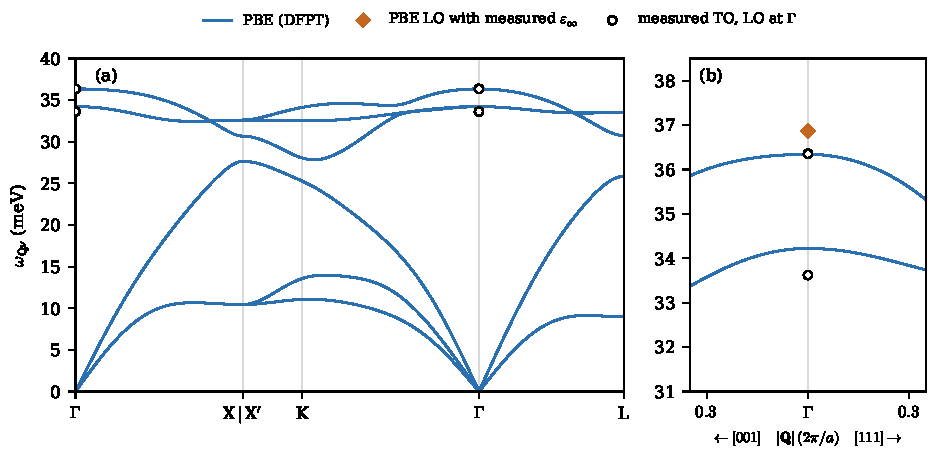
\includegraphics[width=\linewidth]{figures/ch05/fig5_4.pdf}
  \caption{Phonon dispersion of GaAs. (a) Computed along $\mathrm{\Gamma}$--X--K--$\mathrm{\Gamma}$--L with density-functional perturbation theory: PBE functional, SG15 norm-conserving pseudopotentials with the gallium $3d$ shell in the valence, a \SI{60}{Ry} cutoff, an $8^3$ grid of crystal momenta, the static-lattice constant $a = \SI{5.638}{\angstrom}$ of \cref{tab:E-functionals} (the measured value extrapolated to zero temperature with the zero-point expansion removed) and natural masses, on a $4^3$ grid of wavevectors. The force constants are Fourier interpolated with the dipole term of \cref{eq:5.5-na} subtracted and added back, using $\varepsilon_\infty = 13.7$ and $Z^* = 2.094$ computed on a $28^3$ grid of crystal momenta; acoustic sum rules imposed on the force constants and on the Born charges. Circles: measured TO and LO energies at $\mathrm{\Gamma}$, 8.13 and \SI{8.79}{THz}~\cite{strauch1990phonon}, as tabulated in Ref.~\cite[Table~I]{dehghani2025influence}. (b) Optical branches near $\mathrm{\Gamma}$ along $[001]$ (left) and $[111]$ (right), with $|\vect{Q}|$ in units of $2\pi/a$. Diamond: LO energy at $\mathrm{\Gamma}$ from \cref{eq:5.5-LOTO} with the computed TO energy and Born charge and the measured $\varepsilon_\infty = 10.88$~\cite{lockwood2005optical}.}
  \label{fig:5-gaas}
\end{figure}

\Cref{fig:5-gaas} shows the computed phonons of GaAs. The transverse optical energy at $\mathrm{\Gamma}$ comes out at \SI{34.22}{meV}, \SI{1.8}{\percent} above the measured \SI{33.62}{meV}. PBE usually makes phonons slightly soft, but here the measured lattice constant compresses the crystal relative to the PBE minimum at \SI{5.746}{\angstrom} (\cref{tab:E-functionals}). The longitudinal branch meets the zone center at \SI{36.34}{meV} from every direction. In a cubic crystal $Z^*_\kappa\cdot\hat{\vect{Q}} = Z^*_\kappa\hat{\vect{Q}}$ and $\hat{\vect{Q}}\cdot\varepsilon_\infty\cdot\hat{\vect{Q}} = \varepsilon_\infty$ for every $\hat{\vect{Q}}$, and the nonanalytic term does not depend on the direction; in an anisotropic crystal such as sapphire it does, and so does the LO frequency at $\mathrm{\Gamma}$~\cite{griffin2018directional}. The computed splitting is \SI{2.12}{meV} against the measured \SI{2.73}{meV}, \SI{22}{\percent} short, and \cref{eq:5.5-LOTO} shows why. The second term of \cref{eq:5.5-LOTO} is $e^2Z^{*2}/(\Omega\varepsilon_\infty\mu_{\mathrm{red}})$, the Born charge is right to a percent, and $\varepsilon_\infty$ is \SI{26}{\percent} too large. With the measured $\varepsilon_\infty$ and the computed $Z^*$ and $\omega_{\mathrm{T}}$, the same formula yields a splitting of \SI{2.65}{meV}, within \SI{3}{\percent} of the measurement (the diamond in \cref{fig:5-gaas}(b)). The computed LO energy itself agrees with the measured one, but by accident: the transverse energy is high and the splitting short by nearly the same amount. The near-equal masses of gallium and arsenic leave almost no gap between the acoustic and optical bands: the longitudinal acoustic branch ends at \SI{27.65}{meV} at X, and the optical band begins \SI{0.2}{meV} higher.

Because of the nonanalytic term, Fourier interpolation of the force constants needs an extra step in a polar crystal. In real space the dipole--dipole interaction behind \cref{eq:5.5-na} falls off as the inverse cube of the distance, too slowly for any grid of wavevectors to capture, and the computed $D^{\mathrm{dyn}}(\vect{Q})$ near $\mathrm{\Gamma}$ is not smooth. The analytic part $C^{\mathrm{an}}$ is the response with the $\vect{G} = 0$ term of the Coulomb interaction removed~\cite{pick1970microscopic}, and for this reason it can be computed at zero macroscopic field. Since the nonanalytic term is fixed by $Z^*_\kappa$ and $\varepsilon_\infty$ alone, it can be subtracted from the computed matrices in an Ewald-summed form that is periodic in $\vect{Q}$. The short-ranged difference between the computed matrices and this term is then interpolated, and the nonanalytic term is added back analytically at each target $\vect{Q}$~\cite{gonze1997dynamical}. \Cref{fig:5-gaas} was interpolated in this way from a $4^3$ grid.

The electrostatic treatment assumed $|\vect{Q}| \gg \omega/c$. For wavevectors comparable with $\omega/c$, the transverse optical phonon mixes with the photon of the same wavevector and frequency, and the two form the coupled modes called \emph{phonon polaritons}. The crossover happens near $Q \sim \varepsilon_0^{1/2}\omega_{\mathrm{T}}$ in natural units, about \SI{0.1}{eV} for $\omega_{\mathrm{T}} \sim \SI{30}{meV}$ and less than $10^{-4}$ of the size of the zone; at this wavevector the photon line $\omega = Q/\varepsilon_0^{1/2}$ meets the phonon. Dark-matter scattering transfers $q \sim m_\chi v \gtrsim \SI{1}{eV}$ for any mass above a keV, and for the phonons it excites the electrostatic result is exact. Absorption is different. A boson of mass $m$ from the halo, moving at $v \sim 10^{-3}$, deposits $\omega \approx m$ with a momentum of only $mv \sim 10^{-3}\omega$, deep inside the polariton region. The crystal then sees a field that is uniform in space, and the coupling to a uniform field is derived below.

\subsection{The Lyddane--Sachs--Teller relation}

A uniform field oscillating at frequency $\omega$, $\vect{\mathcal{E}}\,\ee^{-\ii\omega t}$, is the opposite limit, $Q \to 0$ at fixed $\omega$, and it measures the dielectric function of the crystal with the lattice included. The field now drives the relative displacement without any longitudinal constraint, to the steady response $\vect{u}_{\mathrm{rel}} = eZ^*\vect{\mathcal{E}}/[\mu_{\mathrm{red}}(\omega_{\mathrm{T}}^2 - \omega^2)]$, and the electrons respond with $\varepsilon_\infty$ as long as $\omega$ lies far below the gap, the adiabatic condition of \cref{sec:5.1}. Inserting $\vect{u}_{\mathrm{rel}}$ into $\vect{P}$ gives the dielectric function $\varepsilon(\omega) = D/\mathcal{E} = 1 + P/\mathcal{E}$ as
\begin{equation}
  \varepsilon(\omega) = \varepsilon_\infty + \frac{e^2Z^{*2}}{\Omega\,\mu_{\mathrm{red}}\,(\omega_{\mathrm{T}}^2 - \omega^2)}
  = \varepsilon_\infty\,\frac{\omega_{\mathrm{L}}^2 - \omega^2}{\omega_{\mathrm{T}}^2 - \omega^2} ,
  \label{eq:5.5-eps}
\end{equation}
where the second form uses \cref{eq:5.5-LOTO} to replace $e^2Z^{*2}/(\Omega\mu_{\mathrm{red}})$ by $\varepsilon_\infty(\omega_{\mathrm{L}}^2 - \omega_{\mathrm{T}}^2)$. At frequencies well above $\omega_{\mathrm{T}}$ the ions cannot follow, and $\varepsilon \to \varepsilon_\infty$; for this reason the electronic dielectric constant is also called the high-frequency dielectric constant (\cref{sec:4.4}). At $\omega = 0$ the ions follow fully and add their polarization. The \emph{static dielectric constant} $\varepsilon_0 = \varepsilon(0)$, lattice included, is $\varepsilon_\infty + e^2Z^{*2}/(\Omega\mu_{\mathrm{red}}\omega_{\mathrm{T}}^2)$, and the second form of \cref{eq:5.5-eps} turns this expression into a relation between measurable quantities alone:
\begin{keyresult}[Lyddane--Sachs--Teller relation]
\begin{equation}
  \frac{\varepsilon_0}{\varepsilon_\infty} = \frac{\omega_{\mathrm{L}}^2}{\omega_{\mathrm{T}}^2} .
  \label{eq:5.5-LST}
\end{equation}
For several polar modes, $\varepsilon_0/\varepsilon_\infty = \prod_\nu\omega_{\mathrm{L}\nu}^2/\omega_{\mathrm{T}\nu}^2$ (\cref{eq:D.14-LSTgen}).
\end{keyresult}
This is the relation of Lyddane, Sachs and Teller~\cite{lyddane1941polar}. The Born charge, the masses and the cell volume have dropped out: the ratio of the two dielectric constants is fixed by the ratio of two frequencies. The general form, with one factor per polar mode, is due to Cochran and Cowley~\cite{cochran1962dielectric}, and follows from the interlacing of the poles and zeros of $\varepsilon(\omega)$.

Those poles and zeros are the content of \cref{eq:5.5-eps}, and they hold beyond the model. The transverse frequency is a pole: a transverse mode creates no field, so it needs none, and it shows up where the response to a field diverges. The longitudinal frequency is a zero. A longitudinal mode has $\vect{\mathcal{E}} \parallel \hat{\vect{Q}}$ and needs $\hat{\vect{Q}}\cdot\vect{D} = \varepsilon(\omega)\,\mathcal{E}_\parallel = 0$, which allows a nonzero field only where $\varepsilon(\omega)$ vanishes. A zero of $\varepsilon(\omega)$ also fixes the plasmon of \cref{sec:4.5}, a self-sustained longitudinal oscillation of the electrons; the LO phonon is a self-sustained longitudinal oscillation of the ions. Between $\omega_{\mathrm{T}}$ and $\omega_{\mathrm{L}}$, \cref{eq:5.5-eps} is negative, no transverse wave propagates, and light in this band, the reststrahlen band, is reflected~\cite[Chap.~27]{ashcroft1976solid}. The loss function $\Imag[-1/\varepsilon(\omega)]$ of \cref{sec:4.4} peaks at $\omega_{\mathrm{L}}$, and the absorption $\varepsilon_2$ at $\omega_{\mathrm{T}}$, once the phonons are given a width.

With several polar modes the steps that led to \cref{eq:5.5-eps} give the general form. Let $\omega_{\mathrm{T}\nu}$ and $\vect{e}_{\kappa\nu}$ be the frequencies and polarization vectors of the analytic problem at $\vect{Q} = 0$, the eigenpairs of $C^{\mathrm{an}}_{\kappa\kappa'}/(M_\kappa M_{\kappa'})^{1/2}$, chosen real. With the expansion $\vect{u}_\kappa = \sum_\nu\vect{e}_{\kappa\nu}a_\nu/\sqrt{M_\kappa}$, each normal coordinate obeys $\ddot a_\nu = -\omega_{\mathrm{T}\nu}^2a_\nu + e\,\vect{z}_\nu\cdot\vect{\mathcal{E}}$, with the mode charge vector $\vect{z}_\nu = \sum_\kappa\vect{e}_{\kappa\nu}\cdot Z^*_\kappa/\sqrt{M_\kappa}$, and it contributes $(e/\Omega)\,a_\nu\vect{z}_\nu$ to the polarization. In a cubic crystal, along any direction $\hat{\vect{e}}$,
\begin{equation*}
  \varepsilon(\omega) = \varepsilon_\infty + \frac{e^2}{\Omega}\sum_\nu\frac{(\vect{z}_\nu\cdot\hat{\vect{e}})^2}{\omega_{\mathrm{T}\nu}^2 - \omega^2} .
\end{equation*}
This is a rational function of $\omega^2$ that tends to $\varepsilon_\infty$ at large $\omega$, has simple poles at the polar transverse frequencies, and, by the argument above, vanishes at the longitudinal frequencies $\omega_{\mathrm{L}\nu}$. Between two consecutive poles it rises monotonically from $-\infty$ to $+\infty$, and above the highest pole it rises from $-\infty$ toward $\varepsilon_\infty$, so there is exactly one zero above each pole and below the next. A rational function is fixed by its poles, its zeros and its limit at infinity, so $\varepsilon(\omega) = \varepsilon_\infty\prod_\nu(\omega_{\mathrm{L}\nu}^2 - \omega^2)/(\omega_{\mathrm{T}\nu}^2 - \omega^2)$, and at $\omega = 0$
\begin{equation}
  \frac{\varepsilon_0}{\varepsilon_\infty} = \prod_\nu\frac{\omega_{\mathrm{L}\nu}^2}{\omega_{\mathrm{T}\nu}^2} ,
  \label{eq:D.14-LSTgen}
\end{equation}
which generalizes \cref{eq:5.5-LST}.

\begin{workedexample}{The Lyddane--Sachs--Teller relation for GaAs}\label{we:5-lst}
We test \cref{eq:5.5-LST} on measured numbers. Neutron scattering puts the optical phonons of GaAs at $\omega_{\mathrm{T}} = \SI{8.13}{THz} = \SI{33.62}{meV}$ and $\omega_{\mathrm{L}} = \SI{8.79}{THz} = \SI{36.35}{meV}$~\cite{strauch1990phonon}, as tabulated in Ref.~\cite[Table~I]{dehghani2025influence}, and infrared spectroscopy measured $\varepsilon_0 = 12.9$ and $\varepsilon_\infty = 10.88$~\cite{lockwood2005optical}, as quoted in Ref.~\cite{knapen2018detection}.

\emph{The relation.} The two sides are
\begin{equation*}
  \frac{\varepsilon_0}{\varepsilon_\infty} = \frac{12.9}{10.88} = 1.186 , \qquad
  \frac{\omega_{\mathrm{L}}^2}{\omega_{\mathrm{T}}^2} = \Bigl(\frac{8.79}{8.13}\Bigr)^2 = 1.169 ,
\end{equation*}
equal to \SI{1.4}{\percent}. Read as a prediction, the relation puts the longitudinal phonon at $\omega_{\mathrm{L}} = \omega_{\mathrm{T}}(\varepsilon_0/\varepsilon_\infty)^{1/2}$, or \SI{36.61}{meV}, \SI{0.26}{meV} or \SI{0.7}{\percent} above the measurement. The splitting itself comes out as \SI{2.99}{meV} against \SI{2.73}{meV}, \SI{9}{\percent} high. The relative error grows because the ratio is close to one: $\omega_{\mathrm{L}}^2 - \omega_{\mathrm{T}}^2$ is $0.17\,\omega_{\mathrm{T}}^2$, and a \SI{1.4}{\percent} error in the ratio is a \SI{10}{\percent} error in that difference. For a harmonic crystal with adiabatic electrons the relation is exact. The \SI{1.4}{\percent} mismatch between the two sides therefore comes from the inputs. The four numbers come from different measurements on different samples, and the dielectric constants of GaAs change at the percent level between room temperature and liquid-helium temperature~\cite{griffin2018directional}.

\emph{The Born charge.} Solved for the Born charge, \cref{eq:5.5-LOTO} reads $Z^{*2} = \Omega\varepsilon_\infty\mu_{\mathrm{red}}(\omega_{\mathrm{L}}^2 - \omega_{\mathrm{T}}^2)/e^2$. With $a = \SI{5.638}{\angstrom}$, $\Omega = a^3/4 = \SI{44.80}{\angstrom^3} = \SI{5.831e-9}{eV^{-3}}$ in natural units, the masses 69.723 and \SI{74.922}{u}, so that $\mu_{\mathrm{red}} = \SI{36.11}{u} = \SI{33.64}{GeV}$, $e^2 = 4\pi\alpha = 0.0917$ and $\omega_{\mathrm{L}}^2 - \omega_{\mathrm{T}}^2 = \SI{1.910e-4}{eV^2}$,
\begin{equation*}
  Z^* = \Bigl[\frac{(5.831\times10^{-9})\times10.88\times(3.364\times10^{10})\times(1.910\times10^{-4})}{0.0917}\Bigr]^{1/2} = 2.11 .
\end{equation*}
The static constant offers a second route, since \cref{eq:5.5-eps} at $\omega = 0$ gives $\varepsilon_0 - \varepsilon_\infty = e^2Z^{*2}/(\Omega\mu_{\mathrm{red}}\omega_{\mathrm{T}}^2)$. The second route yields 2.21, \SI{5}{\percent} more: the same \SI{1.4}{\percent} inconsistency of the inputs magnified by the difference $\varepsilon_0 - \varepsilon_\infty = 2.02$. The splitting, measured directly by one experiment, is the better input.

\emph{Against the calculation.} The converged PBE Born charge, 2.094, lies \SI{0.7}{\percent} below the value just extracted, while the PBE $\varepsilon_\infty$, 13.7, lies \SI{26}{\percent} above the measurement; the error in $\varepsilon_\infty$ is why the computed splitting of \cref{fig:5-gaas} falls short. Wherever a rate needs the combination $Z^{*2}/\varepsilon_\infty$, the measured splitting, or the computed Born charge with the measured $\varepsilon_\infty$, is the input to use.
\end{workedexample}

\subsection{Coupling to a uniform field}

The middle term of \cref{eq:5.5-U}, $-e\sum_\kappa\vect{u}_\kappa\cdot Z^*_\kappa\cdot\vect{\mathcal{E}}$, is the energy of the dipoles of the displaced sublattices in the field. For a field uniform over the crystal and slow compared with the electrons, it adds a term to the nuclear Hamiltonian of \cref{eq:5.3-H}:
\begin{equation*}
  H_{\mathcal{E}}(t) = -e\sum_{\vect{R}\kappa}\vect{u}_{\vect{R}\kappa}\cdot Z^*_\kappa\cdot\vect{\mathcal{E}}(t) .
\end{equation*}
When the phonon expansion \cref{eq:5.3-u} is inserted, the lattice sum $\sum_{\vect{R}}\ee^{\ii\vect{Q}\cdot\vect{R}} = N\delta_{\vect{Q},0}$ keeps only the modes at the zone center:
\begin{equation}
  H_{\mathcal{E}}(t) = -e\sqrt{N}\sum_\nu\frac{\vect{z}_\nu\cdot\vect{\mathcal{E}}(t)}{\sqrt{2\omega_{0\nu}}}\,B_{0\nu} ,
  \qquad
  \vect{z}_\nu = \sum_\kappa\frac{\vect{e}_{\kappa\nu}(0)\cdot Z^*_\kappa}{\sqrt{M_\kappa}} ,
  \label{eq:5.5-HE}
\end{equation}
with $\vect{z}_\nu$ the mode charge vector and $\omega_{0\nu}$ the frequency of branch $\nu$ at $\mathrm{\Gamma}$. The amplitude to create one phonon from the ground state, by \cref{eq:5.3-me}, is $-e\sqrt N\,\vect{z}_\nu\cdot\vect{\mathcal{E}}/\sqrt{2\omega_{0\nu}}$.

In \cref{eq:5.5-HE} the acoustic modes do not couple. At $\mathrm{\Gamma}$ their polarization vectors are $(M_\kappa/M_{\mathrm{cell}})^{1/2}\hat{\vect{e}}$ (\cref{sec:5.2}), so that $\vect{z}_\nu = \hat{\vect{e}}\cdot\sum_\kappa Z^*_\kappa/\sqrt{M_{\mathrm{cell}}}$, which vanishes by the charge neutrality \cref{eq:5.5-neutral}: a uniform field cannot push a neutral crystal. In GaAs the optical modes at $\mathrm{\Gamma}$ have $\vect{e}_{1} = (M_2/M_{\mathrm{cell}})^{1/2}\hat{\vect{e}}$ and $\vect{e}_{2} = -(M_1/M_{\mathrm{cell}})^{1/2}\hat{\vect{e}}$, and the same algebra as in \cref{app:D.14} leads to $\vect{z}_\nu = Z^*\hat{\vect{e}}/\sqrt{\mu_{\mathrm{red}}}$: the field couples to the optical mode polarized along it, through the Born charge and the reduced mass. The squared amplitude is proportional to $N$. All cells are driven in phase, the whole crystal absorbs the quantum, and the rate grows with the target mass, as for the single-phonon amplitude of \cref{sec:5.3}, without the momentum transfer that a scattering process has to supply.

Which resonance a probe excites depends on what it holds fixed. A field $\vect{\mathcal{E}}$ imposed inside the crystal drives the transverse resonance, the pole of $\varepsilon$ at $\omega_{\mathrm{T}}$. A probe that fixes the source of $\vect{D}$, as a moving charge does, sees $1/\varepsilon$ and excites the longitudinal mode at the zero of $\varepsilon$, $\omega_{\mathrm{L}}$. A dark photon couples through its in-medium mixing with the photon. For a dark photon at rest, of mass $m = \omega$, the medium screens that mixing by $1/\varepsilon(\omega)$: the absorption rate is the photon absorption $\omega\Imag\varepsilon$ times the screened coupling $1/|\varepsilon|^2$, and so proportional to the loss function $\Imag[-1/\varepsilon(\omega)]$~\cite[Eqs.~(2) and~(3)]{knapen2018detection}, which peaks at the zero of $\varepsilon$, $\omega_{\mathrm{L}}$. The absorption of dark-photon dark matter in GaAs therefore peaks at the LO energy, and \cref{chap:11} works out the rate. The longitudinal field also acts on the electrons. Its potential, which grows as $1/Q$ at small $Q$, is the Fr\"ohlich coupling, with a strength set by $\omega_{\mathrm{L}}$ and $1/\varepsilon_\infty - 1/\varepsilon_0$ (\cref{eq:6.2-frohlich}).

The five numbers of this section, $Z^*$, $\varepsilon_\infty$, $\varepsilon_0$, $\omega_{\mathrm{T}}$ and $\omega_{\mathrm{L}}$, obey two relations, \cref{eq:5.5-LOTO,eq:5.5-LST}, so that any three fix the other two.

\section{Displacement correlations}\label{sec:5.6}

A dark-matter particle that transfers \SI{50}{keV} of momentum to a silicon nucleus in a cold crystal pushes on a particle that is spread over \SI{0.05}{\angstrom} by its zero-point motion. The phase $\vect{q}\cdot\vect{u}$ that the push imprints then varies by more than a radian across the nuclear wavefunction, and the expansion of $\ee^{\ii\vect{q}\cdot\vect{u}}$ to first order, which gave the single-phonon amplitude of \cref{sec:5.3}, no longer holds. In some events the nucleus takes up the momentum and the crystal is left in its ground state. Otherwise it emits one phonon, or two, or more, and at large enough momentum transfer the many-phonon sum turns into the free recoil of a lone nucleus. To find out how often each happens, we need the thermal averages of exponentials of displacements, at one time and at two. For a harmonic crystal both are exponentials of quadratic forms in $\vect{q}$, the Debye--Waller exponent $2W_\kappa(\vect{q})$ and the displacement correlation $\mathcal{C}_{\kappa\kappa'}(t)$, and both follow from the tensor $B_\kappa$ and the phonon modes of \cref{sec:5.3}. The same algebra describes the optical spectrum of a localized electron whose transition moves the nuclei around it, where it leads to the Franck--Condon factors and the Huang--Rhys factor.

\subsection{The Bloch identity}

The operator through which a momentum transfer $\vect{q}$ acts on the nucleus $\kappa$ in cell $\vect{R}$ is $\ee^{\ii\vect{q}\cdot\vect{X}}$, with $\vect{X} = \vect{R} + \vect{\tau}_\kappa + \vect{u}_{\vect{R}\kappa}$ (\cref{eq:5.1-X}). The lattice position contributes a phase, and the displacement contributes the operator $\ee^{\ii\vect{q}\cdot\vect{u}_{\vect{R}\kappa}}$. By \cref{eq:5.3-u}, $\vect{q}\cdot\vect{u}_{\vect{R}\kappa}$ is a linear combination of the phonon operators $b_{\vect{Q}\nu}$ and $b^\dagger_{\vect{Q}\nu}$. Its exponential contains every power of them and connects the thermal state to states with any number of extra phonons. The first question is its average.

For a classical Gaussian variable $x$ with zero mean, the average of $\ee^{\ii qx}$ is $\ee^{-q^2\langle x^2\rangle/2}$ (\cref{eq:C.6-generating}). A harmonic crystal in thermal equilibrium makes the same statement for operators. Its density matrix $\ee^{-\beta H_{\mathrm{N}}}/\mathcal{Z}$ is Gaussian in the normal coordinates and momenta, because $H_{\mathrm{N}}$ of \cref{eq:5.3-Hb} is quadratic in them. For any operator $\op{A}$ linear in the phonon operators,
\begin{equation*}
  \langle\ee^{\op{A}}\rangle = \ee^{\langle\op{A}^2\rangle/2} ,
\end{equation*}
which is Bloch's identity, \cref{eq:C.6-bloch}. Expanded in powers of $\op{A}$, it is Wick's theorem: the average of $\op{A}^{2n}$ is the sum over the $(2n)!/(2^nn!)$ ways of pairing the $2n$ factors, each pair worth $\langle\op{A}^2\rangle$.

To prove it, take one oscillator, $H = \omega_0(d^\dagger d + \tfrac12)$ as in \cref{app:C.6}, in thermal equilibrium at temperature $T = 1/\beta$, with $n_{\mathrm{B}} = n_{\mathrm{B}}(\omega_0)$, and let $\op{A} = \eta_1d + \eta_2d^\dagger$ with arbitrary complex $\eta_1$ and $\eta_2$, so that $\op{A}$ need not be Hermitian. Consider $F(\theta) = \langle\ee^{\theta\op{A}}\rangle$ as a function of a real parameter $\theta$. The proof uses two facts. The commutators $[\op{A}, d] = -\eta_2$ and $[\op{A}, d^\dagger] = \eta_1$ are numbers. By \cref{eq:C.6-hadamard}, the transformation by $\ee^{\theta\op{A}}$ therefore only shifts the ladder operators,
\begin{equation*}
  d\,\ee^{\theta\op{A}} = \ee^{\theta\op{A}}\,(d + \theta\eta_2), \qquad d^\dagger\,\ee^{\theta\op{A}} = \ee^{\theta\op{A}}\,(d^\dagger - \theta\eta_1) .
\end{equation*}
The cyclic property of the trace, in turn, moves a ladder operator past the Boltzmann factor at a known cost, as in the proof of Wick's theorem in \cref{app:D.11}: $d\,\ee^{-\beta H} = \ee^{-\beta\omega_0}\ee^{-\beta H}d$, since removing a quantum lowers $H$ by $\omega_0$, and $d^\dagger\ee^{-\beta H} = \ee^{+\beta\omega_0}\ee^{-\beta H}d^\dagger$. As a result, $\langle\ee^{\theta\op{A}}d\rangle = \Tr[d\,\ee^{-\beta H}\ee^{\theta\op{A}}]/\mathcal{Z} = \ee^{-\beta\omega_0}\langle d\,\ee^{\theta\op{A}}\rangle$, and combined with the shift,
\begin{equation*}
  \langle d\,\ee^{\theta\op{A}}\rangle = \ee^{-\beta\omega_0}\langle d\,\ee^{\theta\op{A}}\rangle + \theta\eta_2F(\theta), \qquad
  \langle d\,\ee^{\theta\op{A}}\rangle = \frac{\theta\eta_2F(\theta)}{1 - \ee^{-\beta\omega_0}} = \theta\eta_2\,(n_{\mathrm{B}} + 1)\,F(\theta) .
\end{equation*}
The same steps for $d^\dagger$ give $\langle d^\dagger\ee^{\theta\op{A}}\rangle = \ee^{\beta\omega_0}\langle d^\dagger\ee^{\theta\op{A}}\rangle - \theta\eta_1F(\theta)$, and $\langle d^\dagger\ee^{\theta\op{A}}\rangle = \theta\eta_1\,n_{\mathrm{B}}\,F(\theta)$. The derivative of $F$ is then
\begin{equation*}
  F'(\theta) = \eta_1\langle d\,\ee^{\theta\op{A}}\rangle + \eta_2\langle d^\dagger\ee^{\theta\op{A}}\rangle = \theta\,\eta_1\eta_2\,(2n_{\mathrm{B}} + 1)\,F(\theta) = \theta\,\langle\op{A}^2\rangle\,F(\theta) ,
\end{equation*}
since $\langle\op{A}^2\rangle = \eta_1\eta_2\langle dd^\dagger + d^\dagger d\rangle = \eta_1\eta_2(2n_{\mathrm{B}} + 1)$, the averages of $d^2$ and $d^{\dagger2}$ being zero. With $F(0) = 1$ the solution is $F(\theta) = \ee^{\theta^2\langle\op{A}^2\rangle/2}$, which at $\theta = 1$ is Bloch's identity. For several independent modes in thermal equilibrium, $\op{A} = \sum_\gamma\op{A}_\gamma$ is a sum of commuting pieces, one per mode, the exponential factorizes, and the average in the Gibbs state of \cref{sec:2.5} factorizes too. The exponents add, and $\sum_\gamma\langle\op{A}_\gamma^2\rangle = \langle\op{A}^2\rangle$, because the cross terms $\langle\op{A}_\gamma\op{A}_{\gamma'}\rangle = \langle\op{A}_\gamma\rangle\langle\op{A}_{\gamma'}\rangle$ vanish for $\gamma \ne \gamma'$. The identity therefore holds for any $\op{A}$ linear in the operators of a set of harmonic modes.

The hypotheses are the ones the proof used. The operator must be linear in $d$ and $d^\dagger$, so that its commutators are numbers, and the state must be the thermal state of a quadratic Hamiltonian, so that the trace moves each ladder operator at the cost of a number. In an anharmonic crystal neither holds exactly. The logarithm of $\langle\ee^{\op{A}}\rangle$ is then a series in the cumulants of $\op{A}$, of which the harmonic crystal has only the second. The anharmonic terms of \cref{sec:5.7} make the fourth cumulant nonzero, and the Debye--Waller exponent acquires a correction that grows with temperature faster than $T$.

With $\op{A} = \ii\vect{q}\cdot\vect{u}_{\vect{R}\kappa}$, $\langle\op{A}^2\rangle = -\langle(\vect{q}\cdot\vect{u}_{\vect{R}\kappa})^2\rangle = -\sum_{\alpha\beta}q^\alpha B^{\alpha\beta}_\kappa q^\beta$, with the displacement tensor $B_\kappa$ of \cref{eq:5.3-B}.
\begin{keyresult}[Debye--Waller factor]
For a nucleus $\kappa$ of a harmonic crystal in thermal equilibrium,
\begin{equation}
  \bigl\langle\ee^{\ii\vect{q}\cdot\vect{u}_{\vect{R}\kappa}}\bigr\rangle = \ee^{-W_\kappa(\vect{q})} , \qquad
  2W_\kappa(\vect{q}) = \vect{q}\cdot B_\kappa\cdot\vect{q} = \frac1N\sum_{\vect{Q}\nu}\frac{|\vect{q}\cdot\vect{e}_{\kappa\nu}(\vect{Q})|^2}{2M_\kappa\,\omega_{\vect{Q}\nu}}\,\coth\frac{\omega_{\vect{Q}\nu}}{2T} ,
  \label{eq:5.6-W}
\end{equation}
the same in every cell. At a site of cubic symmetry, $2W_\kappa(\vect{q}) = q^2\langle u_x^2\rangle$.
\end{keyresult}
The factor $\ee^{-W_\kappa}$ is an amplitude: the probability amplitude for the nucleus to absorb $\vect{q}$ and leave the lattice in the state it found it in, averaged over that state. The probability is its square, the \emph{Debye--Waller factor} $\ee^{-2W_\kappa(\vect{q})}$, and $W_\kappa(\vect{q})$ is the Debye--Waller exponent. In X-ray and neutron diffraction the factor multiplies the intensity of every Bragg peak, which is how $B_\kappa$ is measured; in silicon at \SI{293}{K}, with the reference value $\langle u_x^2\rangle = \SI{5.94e-3}{\angstrom^2}$ of \cref{we:5-u2}, it reduces the (111) reflection, at $|\vect{G}_{111}| = \sqrt3\,2\pi/a = \SI{3.95}{keV}$, by only \SI{2.4}{\percent}. Note that the electron--phonon literature also uses the name ``Debye--Waller'' for the term of second order in the displacements of the electron--phonon interaction. That term shifts electronic energies and is a different object, the Allen--Heine term of \cref{sec:6.3} (\cref{app:A.6}); in this book the name means \cref{eq:5.6-W} only.

\Cref{eq:5.6-W} inherits the structure of $B_\kappa$. The exponent grows as $q^2$, and it is largest along directions in which the nucleus is soft. Each mode contributes in proportion to the projection of $\vect{q}$ on its polarization, divided by its energy, and weighted by $2n_{\vect{Q}\nu} + 1$, which grows from one at $T = 0$ to $2T/\omega_{\vect{Q}\nu}$ at high temperature. For one species at a cubic site, $2W_\kappa = q^2\langle u^2\rangle/3$, and in the Debye model \cref{eq:5.3-debye} gives
\begin{equation}
  2W_\kappa(\vect{q}) = \frac{3q^2}{4M_\kappa\omega_{\mathrm{D}}}\Bigl[1 + 4\Bigl(\frac{T}{\omega_{\mathrm{D}}}\Bigr)^2\int_0^{\omega_{\mathrm{D}}/T}\frac{x\,\dd x}{\ee^x - 1}\Bigr] .
  \label{eq:D.15-debye}
\end{equation}
At $T = \omega_{\mathrm{D}}$ the bracket is $4.11$: the exponent is four times its zero-point value. At $T = 0$ it is
\begin{equation*}
  2W_\kappa(\vect{q}) = \frac{3q^2}{4M_\kappa\omega_{\mathrm{D}}} = \frac32\,\frac{E_R}{\omega_{\mathrm{D}}} , \qquad E_R = \frac{q^2}{2M_\kappa} ,
\end{equation*}
with $E_R$ the recoil energy that a free nucleus would take (\cref{sec:1.3}). This is the scale that controls everything below: the lattice stays in its ground state with high probability as long as the recoil energy is small compared with typical phonon energies, and almost never once it is large. For numbers we use the computed spectrum, since the Debye model misses the flat transverse acoustic branches (\cref{we:5-u2}).

\subsection{The displacement correlation}

A scattering rate needs more than an average. By \cref{eq:4.2-Sab}, the dynamic structure factor of the nuclei is the Fourier transform in time of the correlation of the density operator at time $t$ with its adjoint at time zero. For one nucleus the density is $\ee^{\ii\vect{q}\cdot\vect{X}}$, and the static phases cancel between the two factors, leaving
\begin{equation*}
  \bigl\langle\ee^{-\ii\vect{q}\cdot\vect{u}_{\vect{R}\kappa}(t)}\,\ee^{\ii\vect{q}\cdot\vect{u}_{\vect{R}\kappa}(0)}\bigr\rangle ,
\end{equation*}
with the Heisenberg operators $b_{\vect{Q}\nu}(t) = b_{\vect{Q}\nu}\ee^{-\ii\omega_{\vect{Q}\nu}t}$ of \cref{sec:5.3}. The two exponents are still linear in the phonon operators, but they do not commute, and Bloch's identity has to be combined with the Baker--Campbell--Hausdorff formula. For two operators $\op{A}$ and $\op{B}$ linear in the phonon operators, the commutator is a number, $\ee^{\op{A}}\ee^{\op{B}} = \ee^{\op{A} + \op{B}}\ee^{[\op{A}, \op{B}]/2}$ (\cref{eq:C.6-BCH}), and Bloch's identity applied to $\op{A} + \op{B}$ leads to
\begin{equation*}
  \langle\ee^{\op{A}}\ee^{\op{B}}\rangle = \exp\Bigl[\tfrac12\langle\op{A}^2\rangle + \tfrac12\langle\op{B}^2\rangle + \langle\op{A}\op{B}\rangle\Bigr] ,
\end{equation*}
\cref{eq:C.6-product}. With $\op{A} = -\ii\vect{q}\cdot\vect{u}_{\vect{R}\kappa}(t)$ and $\op{B} = \ii\vect{q}\cdot\vect{u}_{\vect{R}\kappa}(0)$, the first two terms are $-W_\kappa(\vect{q})$ each, since the thermal state is stationary and the average of a square does not depend on time. The third term is a correlation of two displacements at different times. Inserting \cref{eq:5.3-u} twice, the averages $\langle b_{\vect{Q}\nu}b^\dagger_{\vect{Q}\nu}\rangle = n_{\vect{Q}\nu} + 1$ and $\langle b^\dagger_{\vect{Q}\nu}b_{\vect{Q}\nu}\rangle = n_{\vect{Q}\nu}$ now come with the phases $\ee^{-\ii\omega_{\vect{Q}\nu}t}$ and $\ee^{+\ii\omega_{\vect{Q}\nu}t}$, and the \emph{displacement correlation} of the nuclei $\kappa$ and $\kappa'$ is
\begin{equation}
  \mathcal{C}^{\alpha\beta}_{\kappa\kappa'}(\vect{R},t) = \bigl\langle u^\alpha_{\vect{R}\kappa}(t)\,u^\beta_{\vect{0}\kappa'}(0)\bigr\rangle
  = \frac1N\sum_{\vect{Q}\nu}\frac{e^\alpha_{\kappa\nu}(\vect{Q})\,e^\beta_{\kappa'\nu}(\vect{Q})^*\,\ee^{\ii\vect{Q}\cdot\vect{R}}}{2\omega_{\vect{Q}\nu}\sqrt{M_\kappa M_{\kappa'}}}\Bigl[(n_{\vect{Q}\nu} + 1)\,\ee^{-\ii\omega_{\vect{Q}\nu}t} + n_{\vect{Q}\nu}\,\ee^{\ii\omega_{\vect{Q}\nu}t}\Bigr] ,
  \label{eq:5.6-C}
\end{equation}
For one nucleus, $\vect{R} = \vect{0}$ and $\kappa' = \kappa$, we write $\mathcal{C}_{\kappa\kappa}(t)$. Its value at $t = 0$ is the displacement tensor, $\mathcal{C}_{\kappa\kappa}(0) = B_\kappa$. The term with $n_{\vect{Q}\nu} + 1$ creates a phonon at time zero and removes it at time $t$, and oscillates at the positive frequency $\omega_{\vect{Q}\nu}$; the term with $n_{\vect{Q}\nu}$ absorbs a thermal phonon first, and it vanishes at $T = 0$. Unlike $B_\kappa$, the correlation is complex, because $\vect{u}(t)$ and $\vect{u}(0)$ do not commute. Its imaginary part, $\Imag\mathcal{C}_{\kappa\kappa}(t) = -\sum_{\vect{Q}\nu}\vect{e}_{\kappa\nu}\vect{e}^*_{\kappa\nu}\sin(\omega_{\vect{Q}\nu}t)/(2NM_\kappa\omega_{\vect{Q}\nu})$, does not depend on temperature; we will see that it carries the recoil energy.
\begin{keyresult}[Generating formula]
For a nucleus $\kappa$ of a harmonic crystal in thermal equilibrium,
\begin{equation}
  \bigl\langle\ee^{-\ii\vect{q}\cdot\vect{u}_{\vect{R}\kappa}(t)}\,\ee^{\ii\vect{q}\cdot\vect{u}_{\vect{R}\kappa}(0)}\bigr\rangle
  = \ee^{-2W_\kappa(\vect{q})}\;\ee^{\vect{q}\cdot\mathcal{C}_{\kappa\kappa}(t)\cdot\vect{q}} ,
  \label{eq:5.6-gen}
\end{equation}
with $2W_\kappa$ of \cref{eq:5.6-W} and $\mathcal{C}_{\kappa\kappa}(t)$ of \cref{eq:5.6-C}. For two nuclei in different cells or sublattices, by the same steps,
\begin{equation}
  \bigl\langle\ee^{-\ii\vect{q}\cdot\vect{u}_{\vect{R}\kappa}(t)}\,\ee^{\ii\vect{q}\cdot\vect{u}_{\vect{0}\kappa'}(0)}\bigr\rangle = \ee^{-W_\kappa(\vect{q}) - W_{\kappa'}(\vect{q})}\;\ee^{\vect{q}\cdot\mathcal{C}_{\kappa\kappa'}(\vect{R},t)\cdot\vect{q}} .
  \label{eq:D.15-gen}
\end{equation}
\end{keyresult}
This is the starting point of the theory of neutron scattering from crystals~\cite[App.~N]{ashcroft1976solid}, \cite[Chaps.~3 and~4]{lovesey1984theorynuclear}.
The left side equals one at $t = 0$, and so does the right side, since $\vect{q}\cdot\mathcal{C}_{\kappa\kappa}(0)\cdot\vect{q} = 2W_\kappa$. The single-nucleus form, \cref{eq:5.6-gen}, is the \emph{self} part of the nuclear response, in which the same nucleus scatters at both times. The full structure factor of the crystal adds the pairs of different nuclei, whose phases $\ee^{\ii\vect{q}\cdot(\vect{R} + \vect{\tau}_\kappa - \vect{\tau}_{\kappa'})}$ produce the Bragg peaks and the crystal-momentum conservation of the single-phonon amplitude of \cref{sec:5.3}; \cref{sec:11.3} builds the complete response from both.

Both $W_\kappa$ and $\mathcal{C}_{\kappa\kappa'}(t)$ are sums over all phonons of the zone, computed after the phonon calculation from the frequencies and polarization vectors that DFPT yields on a fine grid of wavevectors, by Fourier interpolation of the force constants. The cost of the sums is negligible next to the phonon calculation itself. The acoustic modes near $\mathrm{\Gamma}$ make the summand of $2W_\kappa$ diverge as $1/\omega$ or $1/\omega^2$, and a uniform grid needs the analytic correction of \cref{sec:5.3}. The same small frequencies control $\mathcal{C}_{\kappa\kappa'}(t)$ at long times, which set the shape of the spectrum at small energies.

\subsection{Expansion in phonon number}

Expanding the second exponential of \cref{eq:5.6-gen} in powers of $\vect{q}\cdot\mathcal{C}_{\kappa\kappa}(t)\cdot\vect{q}$ sorts the response by the number of phonons involved. The $n$th power is a sum of products of $n$ factors $\ee^{\mp\ii\omega_{\vect{Q}\nu}t}$, one per phonon created (upper sign) or absorbed (lower sign), and its Fourier transform puts weight at the sums of $n$ phonon energies with these signs. The term $n = 0$ is time independent and is the elastic weight $\ee^{-2W_\kappa}$ at $\omega = 0$. The term $n = 1$ is the single-phonon response of \cref{sec:5.3}, now multiplied by $\ee^{-2W_\kappa}$.

The bookkeeping is simplest at a site of cubic symmetry with one species of nucleus, as in silicon. There $\mathcal{C}_{\kappa\kappa}(t)$ is a multiple of the identity, like $B_\kappa$. Its trace reduces to an integral over the density of states as in \cref{eq:5.3-u2}:
\begin{equation*}
  \vect{q}\cdot\mathcal{C}_{\kappa\kappa}(t)\cdot\vect{q} = \frac{q^2}{3}\int_0^\infty\dd\omega\;\frac{g_{\mathrm{ph}}(\omega)}{n_{\mathrm{at}}}\,\frac{(n_{\mathrm{B}}(\omega) + 1)\,\ee^{-\ii\omega t} + n_{\mathrm{B}}(\omega)\,\ee^{\ii\omega t}}{2M_\kappa\,\omega}
  = 2W_\kappa(\vect{q})\int_{-\infty}^{\infty}\dd\omega\;P_1(\omega)\,\ee^{-\ii\omega t} .
\end{equation*}
Here $P_1(\omega)$ is the single-phonon distribution, proportional to $g_{\mathrm{ph}}(|\omega|)[n_{\mathrm{B}}(\omega) + 1]/\omega$ for both signs of $\omega$ and normalized to one; at negative $\omega$, $n_{\mathrm{B}}(\omega) + 1 = -n_{\mathrm{B}}(|\omega|)$ gives the absorption weight. The prefactor is $2W_\kappa$, since at $t = 0$ the left side is $\vect{q}\cdot B_\kappa\cdot\vect{q}$. Each power of the exponential is then a convolution in frequency, and the Fourier transform of \cref{eq:5.6-gen} becomes
\begin{equation}
  \int_{-\infty}^{\infty}\dd t\;\ee^{\ii\omega t}\,\ee^{-2W_\kappa}\,\ee^{\vect{q}\cdot\mathcal{C}_{\kappa\kappa}(t)\cdot\vect{q}}
  = 2\pi\,\ee^{-2W_\kappa}\sum_{n=0}^{\infty}\frac{(2W_\kappa)^n}{n!}\,P_n(\omega) ,
  \label{eq:5.6-multi}
\end{equation}
with $P_0(\omega) = \delta(\omega)$ and $P_n$ the $n$-fold convolution of $P_1$ with itself, normalized to one. The shape of each term comes from the phonon spectrum; its weight does not. The probability that a momentum transfer $\vect{q}$ to one nucleus involves $n$ phonons is the Poisson distribution
\begin{equation}
  p^{\mathrm{ph}}_n = \ee^{-2W_\kappa(\vect{q})}\,\frac{[2W_\kappa(\vect{q})]^n}{n!} ,
  \label{eq:5.6-poisson}
\end{equation}
with mean $2W_\kappa$. At $T = 0$ every phonon is created, $P_1$ lives at positive $\omega$, and $n$ is the number of phonons emitted. At $T > 0$, $n$ counts creations and absorptions together, and a term $n = 2$ that absorbs one phonon and emits another lands near $\omega = 0$. \Cref{eq:5.6-poisson} is the oscillator result \cref{eq:C.6-coherent} for a momentum kick, distributed over all the modes of the crystal: a kick is a displacement in momentum, and the number of quanta it creates out of a Gaussian state is Poisson distributed.

The mean energy deposited takes no calculation at all. The first-moment identity \cref{eq:4.3-firstmoment} fixes it by a double commutator, and for $\op{O} = \ee^{\ii\vect{q}\cdot\vect{X}}$ only the kinetic energy $\vect{p}^2/2M_\kappa$ of the nucleus fails to commute with $\op{O}$. With $\ee^{\ii\vect{q}\cdot\vect{X}}\,\vect{p}\,\ee^{-\ii\vect{q}\cdot\vect{X}} = \vect{p} - \vect{q}$, the commutator is $[\vect{p}^2/2M_\kappa, \op{O}] = \op{O}\,(\vect{q}\cdot\vect{p}/M_\kappa + q^2/2M_\kappa)$, and the double commutator is the number $[\op{O}^\dagger, [H, \op{O}]] = q^2/M_\kappa$. The self response is even in $\vect{q}$, since it depends on $\vect{q}$ only through quadratic forms, so the two terms on the right of \cref{eq:4.3-firstmoment} are equal. Since the weights of \cref{eq:5.6-multi} add up to one, the mean energy deposited is
\begin{equation}
  \ee^{-2W_\kappa}\sum_{n=0}^{\infty}\frac{(2W_\kappa)^n}{n!}\int_{-\infty}^{\infty}\dd\omega\;\omega\,P_n(\omega) = \frac{q^2}{2M_\kappa} = E_R .
  \label{eq:5.6-sum}
\end{equation}
The average energy left in the lattice is the free recoil energy, at every $q$ and every temperature, whatever the force constants. The derivation used only the kinetic energy of the nucleus, not the harmonic approximation or the phonon modes, so the identity holds on any potential-energy surface, anharmonic ones included. In \cref{eq:5.6-gen} it appears as the slope at $t = 0$. The polarization vectors are complete at each $\vect{Q}$ (\cref{eq:5.2-ortho}), $\sum_\nu e^\alpha_{\kappa\nu}(\vect{Q})e^\beta_{\kappa\nu}(\vect{Q})^* = \delta_{\alpha\beta}$, and the derivative of \cref{eq:5.6-C} at $t = 0$ is therefore $-\ii\,\mathbf{1}/2M_\kappa$. The thermal factors cancel between creation and absorption, as for the single oscillator of \cref{we:2-oscillator}, and $\ii\,\dd/\dd t$ of \cref{eq:5.6-gen} at $t = 0$ is $q^2/2M_\kappa$. The elastic weight $\ee^{-2W_\kappa}$ and the first moment behave oppositely: heating the crystal shrinks the elastic weight, since $2W_\kappa$ grows with $\langle u_x^2\rangle$, but leaves the first moment untouched, since the weight that leaves $\omega = 0$ goes to both signs of $\omega$.

The Poisson weights and the sum rule together lay out the regimes of the nuclear response. While $2W_\kappa \ll 1$, the elastic term dominates the total weight, the single-phonon term carries nearly all the inelastic weight, and the first-order expansion of \cref{sec:5.3} holds. Once $2W_\kappa$ approaches one, two- and three-phonon terms carry a comparable share. For $2W_\kappa \gg 1$, the Poisson distribution peaks at $n \approx 2W_\kappa$ with relative width $(2W_\kappa)^{-1/2}$, the elastic weight is exponentially small, and the spectrum is a broad peak centered at $E_R$, the free recoil of the standard nuclear-recoil rate (\cref{sec:11.4}). At $T = 0$ the mean energy per phonon, $E_R/2W_\kappa = 1/(2M_\kappa\langle u_x^2\rangle)$, is the inverse of the mean of $1/\omega$ over the spectrum, the typical frequency $\langle\omega^{-1}\rangle^{-1}$ of \cref{sec:5.3}. The ratio of the recoil energy to that typical phonon energy is the zero-temperature $2W_\kappa$ itself, and it decides which regime a given momentum transfer is in.

\begin{workedexample}{The Debye--Waller exponent of silicon}\label{we:5-dw}
We take the natural mass of silicon, $M_\kappa = \SI{26.16}{GeV}$, and the values of $\langle u_x^2\rangle$ from \cref{we:5-u2}. The computed density of states gives \SI{2.45e-3}{\angstrom^2} at $T = 0$ and \SI{6.38e-3}{\angstrom^2} at \SI{293}{K}; the lattice-dynamical fit to the measured phonons gives \SI{5.94e-3}{\angstrom^2} at \SI{293}{K}~\cite{flensburg1999lattice}. With $\hbar c = \SI{1973.27}{eV.\angstrom}$, \SI{1}{\angstrom^2} is \SI{2.568e-7}{eV^{-2}}.

\emph{$q = \SI{10}{keV}$.} The recoil energy is $E_R = q^2/2M_\kappa = \SI{1.91}{meV}$, far below the phonon energies. At $T = 0$, $2W_\kappa = q^2\langle u_x^2\rangle = \num{1e8}\times\num{2.45e-3}\times\num{2.568e-7} = 0.063$, the elastic weight is $0.939$, and by \cref{eq:5.6-poisson} one phonon is created with probability $0.059$ and two with probability $0.0019$. At \SI{293}{K}, $2W_\kappa = 0.164$ (0.153 with the reference value) and $\ee^{-2W_\kappa} = 0.85$. A momentum transfer of \SI{10}{keV} is in the single-phonon regime, and the expansion of \cref{sec:5.3} is accurate to the size of the two-phonon term, a few percent of the inelastic weight.

\emph{$q = \SI{50}{keV}$.} The recoil energy is \SI{47.8}{meV}, comparable to the optical phonon. At $T = 0$, $2W_\kappa = 1.57$, and the Poisson weights for zero, one, two, three and four phonons are $0.21$, $0.33$, $0.26$, $0.13$ and $0.05$: almost half of all scatterings, $0.47$, create two or more phonons. The mean energy per phonon is $E_R/2W_\kappa = \SI{30.4}{meV}$, the typical frequency $\langle\omega^{-1}\rangle^{-1}$ of the computed spectrum in \cref{we:5-u2}. At \SI{293}{K}, $2W_\kappa = 4.10$ (3.81 with the reference value), and the elastic weight has dropped to $0.017$.

\emph{Where $2W_\kappa = 1$.} The crossover from the single-phonon to the multiphonon regime sits at $q = \langle u_x^2\rangle^{-1/2}$: \SI{40}{keV} at $T = 0$ and \SI{26}{keV} at \SI{293}{K} with the reference value, the scale anticipated in \cref{sec:5.3}. For a cryogenic detector the first number applies. It is smaller than the \SI{56}{keV} of the single \SI{60}{meV} oscillator of \cref{app:C.6} because the crystal's zero-point motion is set by $\langle\omega^{-1}\rangle^{-1} = \SI{30.4}{meV}$, half the optical energy: the soft transverse acoustic modes move the nucleus most. Indeed, a single oscillator of frequency \SI{30.4}{meV} reproduces the zero-temperature $2W_\kappa$ exactly, since its $|\alpha_{\mathrm{d}}|^2 = E_R/\omega_0$ is then $1/(2M_\kappa\omega_0)\times q^2 = q^2\langle u_x^2\rangle$; it misses only the shape of the spectrum.

\emph{The Debye model.} With $\omega_{\mathrm{D}} = \SI{55.6}{meV}$, \cref{eq:D.15-debye} gives $2W_\kappa = 1.29$ at \SI{50}{keV} and $T = 0$, and \num{2.64} at \SI{293}{K}, low by \SI{18}{\percent} and \SI{35}{\percent}. The elastic weight is correspondingly too large, $0.28$ instead of $0.21$ at $T = 0$, and at room temperature $0.071$ instead of $0.017$, a factor of four. A Debye estimate locates the crossover to within \SI{10}{\percent} in $q$, but a rate that depends on the elastic or single-phonon weight at $2W_\kappa \gtrsim 1$ needs the full spectrum.
\end{workedexample}

\subsection{The displaced oscillator}

An electron bound to a defect in silicon, or to the nitrogen--vacancy center of diamond, absorbs light at one energy and emits it at a lower one. Both spectra show a sharp line with a train of broader replicas spaced by a phonon energy. The reason is that the electronic transition changes the forces on the nearby nuclei. In the language of \cref{sec:5.1}, each electronic state has its own potential-energy surface, and the minima of the two surfaces sit at different nuclear positions. The transition happens at fixed nuclei, and afterwards the nuclei relax to the new minimum and shed the difference as phonons. The momentum kick of \cref{eq:5.6-poisson} displaces the nuclear momentum; the electronic transition displaces the equilibrium position. In both cases the lattice ends up in a displaced Gaussian state, and the same Poisson statistics follow.

The simplest model keeps one vibrational mode, of mass $M$ and frequency $\omega_0$, with the same frequency in both electronic states. In the ground electronic state g and the excited state e the nuclear Hamiltonians are
\begin{equation}
  H_{\mathrm{g}} = \frac{p^2}{2M} + \frac12M\omega_0^2x^2 , \qquad
  H_{\mathrm{e}} = E_{\mathrm{ZPL}} + \frac{p^2}{2M} + \frac12M\omega_0^2(x - \Delta x)^2 ,
  \label{eq:5.6-Hge}
\end{equation}
where $\Delta x$ is the shift of the equilibrium position and $E_{\mathrm{ZPL}}$ the energy between the two minima, the zero-point energies being equal. The difference $H_{\mathrm{e}} - H_{\mathrm{g}}$ is linear in $x$, the linear coupling of the electron to the mode. In the Born--Oppenheimer approximation of \cref{sec:5.1}, the vibronic states are products of an electronic state and an eigenstate of the oscillator that belongs to it. With $x = \ell_0(d + d^\dagger)$ and $\ell_0 = (2M\omega_0)^{-1/2}$ as in \cref{app:C.6}, the displacement operator $\op{D}(\alpha_{\mathrm{d}})$ of \cref{eq:C.6-D} with real $\alpha_{\mathrm{d}} = \Delta x/2\ell_0$ shifts the coordinate by $\Delta x$. Hence $H_{\mathrm{e}} = E_{\mathrm{ZPL}} + \op{D}H_{\mathrm{g}}\op{D}^\dagger$, and the oscillator states of the excited surface are $|m_{\mathrm{e}}\rangle = \op{D}|m\rangle$, with energies $E_{\mathrm{ZPL}} + m\omega_0$ above the ground-state energy of the lower surface (we drop the common $\tfrac12\omega_0$).

An optical transition is driven by the electronic dipole, whose matrix element between g and e depends weakly on the nuclear positions. The Condon approximation takes it constant, and the transition from $|n_{\mathrm{g}}\rangle$ to $|m_{\mathrm{e}}\rangle$ then has a probability proportional to the \emph{Franck--Condon factor} $|\langle m_{\mathrm{e}}|n_{\mathrm{g}}\rangle|^2$, the squared overlap of the two vibrational wavefunctions. From the vibrational ground state, $\langle m_{\mathrm{e}}|0\rangle = \langle m|\op{D}^\dagger|0\rangle = \langle m|\op{D}(-\alpha_{\mathrm{d}})|0\rangle$, and by \cref{eq:C.6-coherent}
\begin{equation}
  |\langle m_{\mathrm{e}}|0_{\mathrm{g}}\rangle|^2 = \ee^{-S_{\mathrm{HR}}}\,\frac{S_{\mathrm{HR}}^m}{m!} , \qquad
  S_{\mathrm{HR}} = \alpha_{\mathrm{d}}^2 = \frac{\Delta x^2}{4\ell_0^2} = \frac{M\omega_0\,\Delta x^2}{2} = \frac{\omega_0\,\Delta Q^2}{2} .
  \label{eq:5.6-FC}
\end{equation}
The \emph{Huang--Rhys factor} $S_{\mathrm{HR}}$~\cite{huang1950theory} is written last with the mass-weighted displacement $\Delta Q = M^{1/2}\Delta x$, the form in which a first-principles calculation supplies it for each mode. It has a direct meaning. The relaxation energy that the lattice releases after a vertical transition, $\tfrac12M\omega_0^2\Delta x^2$, equals $S_{\mathrm{HR}}\,\omega_0$: $S_{\mathrm{HR}}$ is the mean number of phonons emitted in the transition. At $T = 0$ the absorption spectrum is a progression of lines at $E_{\mathrm{ZPL}} + m\omega_0$ with Poisson weights (\cref{fig:5-fc}). The line $m = 0$ is the \emph{zero-phonon line}, with weight $\ee^{-S_{\mathrm{HR}}}$; the lines $m \ge 1$ form the \emph{phonon sideband}. Emission from the relaxed excited state is the mirror image, with lines at $E_{\mathrm{ZPL}} - m\omega_0$ and the same weights. The means of the two spectra lie at $E_{\mathrm{ZPL}} \pm S_{\mathrm{HR}}\omega_0$, and their separation $2S_{\mathrm{HR}}\omega_0$ is the Stokes shift. For $S_{\mathrm{HR}} \ll 1$ the zero-phonon line carries most of the weight; for $S_{\mathrm{HR}} \gg 1$ it is exponentially weak, and the band is a near-Gaussian of width $S_{\mathrm{HR}}^{1/2}\omega_0$ around its mean. Because the weight $\ee^{-S_{\mathrm{HR}}}$ is the fraction of transitions that leave the lattice untouched, the color-center literature calls it the Debye--Waller factor of the line, by analogy with diffraction~\cite[Sect.~2.2]{alkauskas2014first}.

\begin{figure}[tbp]
  \centering
  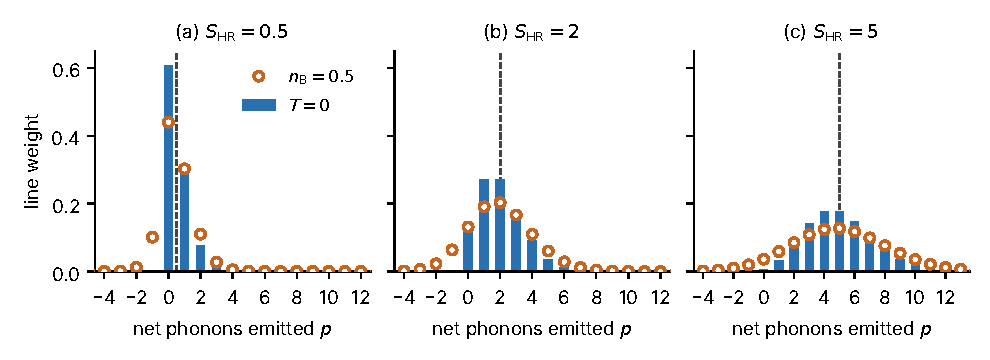
\includegraphics[width=\linewidth]{figures/ch05/fig5_5.pdf}
  \caption{Franck--Condon progressions of a displaced oscillator, for Huang--Rhys factors $S_{\mathrm{HR}} = 0.5$, 2 and 5. Each panel shows the weights of the absorption lines at $E_{\mathrm{ZPL}} + p\,\omega_0$ against the net number $p$ of phonons emitted, for one mode of frequency $\omega_0$ that is the same in both electronic states, in the Condon approximation (dipole independent of the nuclear coordinate). Bars: zero temperature, Poisson weights $\ee^{-S_{\mathrm{HR}}}S_{\mathrm{HR}}^p/p!$; the bar at $p = 0$ is the zero-phonon line. Open circles: mean occupation $n_{\mathrm{B}}(\omega_0) = 0.5$, that is $T = 0.91\,\omega_0$, from the Bessel-function weights of \cref{eq:5.6-bessel}; the lines at $p < 0$ are anti-Stokes lines, which start from thermally excited vibrational states. Dashed line: the mean $p = S_{\mathrm{HR}}$, the same at both temperatures. The zero-phonon fractions at $T = 0$ are 0.61, 0.14 and 0.007.}
  \label{fig:5-fc}
\end{figure}

At finite temperature the initial vibrational state is thermal, and the overlaps $|\langle m_{\mathrm{e}}|n_{\mathrm{g}}\rangle|^2$ for $n > 0$ are needed as well. Summing them with Gibbs weights is a job for the generating function. The absorption line shape is
\begin{equation*}
  \begin{aligned}
  A(E) &= \sum_np_n\sum_m|\langle m_{\mathrm{e}}|n_{\mathrm{g}}\rangle|^2\,\delta\bigl(E - E_{\mathrm{ZPL}} - (m - n)\,\omega_0\bigr) \\
  &= \int_{-\infty}^{\infty}\frac{\dd t}{2\pi}\;\ee^{\ii(E - E_{\mathrm{ZPL}})t}\,\bigl\langle\ee^{\ii H_{\mathrm{g}}t}\op{D}\,\ee^{-\ii H_{\mathrm{g}}t}\op{D}^\dagger\bigr\rangle ,
  \end{aligned}
\end{equation*}
where $p_n$ are the Gibbs weights of the ground-state oscillator (\cref{sec:2.5}). The second form writes each $\delta$-function as the time integral of $\ee^{\ii(E - E_{\mathrm{ZPL}} - m\omega_0 + n\omega_0)t}$, uses $\langle m_{\mathrm{e}}|n_{\mathrm{g}}\rangle = \langle m|\op{D}^\dagger|n\rangle$, and lets $\ee^{\pm\ii H_{\mathrm{g}}t}$ supply the phases $\ee^{\ii n\omega_0t}$ and $\ee^{-\ii m\omega_0t}$; the sum over $m$ is then a completeness sum. The operator $\ee^{\ii H_{\mathrm{g}}t}\op{D}\ee^{-\ii H_{\mathrm{g}}t}$ is $\op{D}$ with $d \to d\,\ee^{-\ii\omega_0t}$, so both exponents are linear in $d$ and $d^\dagger$, and \cref{eq:C.6-product} applies, with $\op{A} = \alpha_{\mathrm{d}}(d^\dagger\ee^{\ii\omega_0t} - d\,\ee^{-\ii\omega_0t})$ and $\op{B} = -\alpha_{\mathrm{d}}(d^\dagger - d)$. The averages are $\langle\op{A}^2\rangle = \langle\op{B}^2\rangle = -S_{\mathrm{HR}}(2n_{\mathrm{B}} + 1)$ and $\langle\op{A}\op{B}\rangle = S_{\mathrm{HR}}[(n_{\mathrm{B}} + 1)\ee^{-\ii\omega_0t} + n_{\mathrm{B}}\ee^{\ii\omega_0t}]$, with $n_{\mathrm{B}} = n_{\mathrm{B}}(\omega_0)$, so that
\begin{equation}
  \bigl\langle\ee^{\ii H_{\mathrm{g}}t}\op{D}\,\ee^{-\ii H_{\mathrm{g}}t}\op{D}^\dagger\bigr\rangle
  = \ee^{-S_{\mathrm{HR}}(2n_{\mathrm{B}} + 1)}\,\exp\Bigl\{S_{\mathrm{HR}}\bigl[(n_{\mathrm{B}} + 1)\,\ee^{-\ii\omega_0t} + n_{\mathrm{B}}\,\ee^{\ii\omega_0t}\bigr]\Bigr\} .
  \label{eq:5.6-Gt}
\end{equation}
It has the form of the generating formula \cref{eq:5.6-gen} for a crystal with a single mode: $2W_\kappa$ becomes $S_{\mathrm{HR}}(2n_{\mathrm{B}} + 1)$, and $\vect{q}\cdot\mathcal{C}_{\kappa\kappa}(t)\cdot\vect{q}$ becomes the second exponent. A kick of momentum $q$ to a single oscillator is the displacement $\op{D}(\ii q\ell_0)$ (\cref{app:C.6}), and it leads to the same expression with $S_{\mathrm{HR}} \to E_R/\omega_0$. The second exponential expands with the generating function of the modified Bessel functions, $\ee^{(z/2)(s + 1/s)} = \sum_ps^pI_p(z)$, taken at $s = [(n_{\mathrm{B}} + 1)/n_{\mathrm{B}}]^{1/2}\ee^{-\ii\omega_0t}$. The coefficient of $\ee^{-\ii p\omega_0t}$ is the weight of the line at $E_{\mathrm{ZPL}} + p\,\omega_0$, for every integer $p$:
\begin{equation}
  w_p = \ee^{-S_{\mathrm{HR}}(2n_{\mathrm{B}} + 1)}\Bigl(\frac{n_{\mathrm{B}} + 1}{n_{\mathrm{B}}}\Bigr)^{p/2}I_p\bigl(2S_{\mathrm{HR}}\sqrt{n_{\mathrm{B}}(n_{\mathrm{B}} + 1)}\bigr) .
  \label{eq:5.6-bessel}
\end{equation}
At $T = 0$ only $p \ge 0$ survives, and $w_p$ returns to the Poisson weights of \cref{eq:5.6-FC}. At $T > 0$ the lines with $p < 0$ appear, and since $I_{-p} = I_p$, $w_{-p}/w_p = \ee^{-p\beta\omega_0}$, detailed balance between the Stokes and anti-Stokes sides. The mean of $p$ is $S_{\mathrm{HR}}$ at every temperature, the slope of \cref{eq:5.6-Gt} at $t = 0$, as the mean recoil energy was in \cref{eq:5.6-sum}.

A real center couples to many modes $k$, each with its own factor $S_k = \omega_k\Delta Q_k^2/2$, and the generating function is the product of factors \cref{eq:5.6-Gt}, one per mode. The total $S_{\mathrm{HR}} = \sum_kS_k$ is the mean number of phonons emitted, and at $T = 0$ the zero-phonon weight is $\ee^{-S_{\mathrm{HR}}}$. With a continuum of modes, the replicas merge into a continuous sideband with the shape of the convolutions of \cref{eq:5.6-multi}, while the zero-phonon line stays sharp, since it involves no phonon. Huang and Rhys derived this structure for the F center of alkali halides, where $S_{\mathrm{HR}}$ is large and the band is broad~\cite{huang1950theory}. \Cref{sec:7.4} applies it to the color centers of silicon and diamond, with their measured Huang--Rhys factors.

\begin{workedexample}{A displaced oscillator}\label{we:5-displaced}
As a toy model we take the bond coordinate of silicon from \cref{sec:5.1}, an oscillator of frequency $\omega_0 = \SI{64.1}{meV}$ whose zero-point length is $\ell_0 = \ell_{\mathrm{zp}} = \SI{0.048}{\angstrom}$ (with the reduced mass $M/2$ of the pair of nuclei, $\ell_0 = (2\cdot\tfrac{M}{2}\cdot\omega_0)^{-1/2}$ is the $\ell_{\mathrm{zp}}$ of \cref{fig:5-scales}). Suppose a localized electronic excitation lengthens the equilibrium bond by $\Delta x$.

\emph{The size of the shift.} A Huang--Rhys factor of two needs $\Delta x = 2\ell_0\sqrt{S_{\mathrm{HR}}} = \SI{0.136}{\angstrom}$, \SI{5.8}{\percent} of the bond length $\sqrt3a/4 = \SI{2.35}{\angstrom}$. A shift of a few times the zero-point length is enough to make the zero-phonon line a minority: the relaxation energy is $S_{\mathrm{HR}}\omega_0 = \SI{128}{meV}$, and the Stokes shift between the means of absorption and emission is \SI{256}{meV}.

\emph{The overlap directly.} The ground-state wavefunction is $\psi_0(x) = (2\pi\ell_0^2)^{-1/4}\ee^{-x^2/4\ell_0^2}$, and the overlap with the same Gaussian centered at $\Delta x$ is
\begin{equation*}
  \langle0_{\mathrm{e}}|0_{\mathrm{g}}\rangle = \frac{1}{\sqrt{2\pi}\,\ell_0}\int\dd x\;\ee^{-[x^2 + (x - \Delta x)^2]/4\ell_0^2}
  = \frac{\ee^{-\Delta x^2/4\ell_0^2}}{\sqrt{2\pi}\,\ell_0}\int\dd x\;\ee^{-x^2/2\ell_0^2 + x\Delta x/2\ell_0^2}
  = \ee^{-\Delta x^2/8\ell_0^2} ,
\end{equation*}
by \cref{eq:C.6-gauss} with $\mu = 1/2\ell_0^2$ and $\eta = \Delta x/2\ell_0^2$, which contributes $\sqrt{2\pi}\,\ell_0\,\ee^{\Delta x^2/8\ell_0^2}$. The squared overlap is $\ee^{-\Delta x^2/4\ell_0^2} = \ee^{-S_{\mathrm{HR}}}$, the zero-phonon weight of \cref{eq:5.6-FC}. For the first replica, $\psi_1(x) = (x/\ell_0)\psi_0(x)$, and the same integral with an extra factor $(x - \Delta x)/\ell_0$ gives $|\langle1_{\mathrm{e}}|0_{\mathrm{g}}\rangle|^2 = S_{\mathrm{HR}}\ee^{-S_{\mathrm{HR}}}$.

\emph{The progression.} For $S_{\mathrm{HR}} = 2$ the weights of the lines with $p = 0$ to 5 phonons are $0.135$, $0.271$, $0.271$, $0.180$, $0.090$ and $0.036$, the middle panel of \cref{fig:5-fc}. The zero-phonon line carries \SI{14}{\percent} of the absorption, and the strongest replicas are those with one and two phonons, which for an integer $S_{\mathrm{HR}}$ are equal.

\emph{Room temperature.} At \SI{300}{K}, $n_{\mathrm{B}}(\omega_0) = 0.091$, the value of \cref{sec:5.3} for the optical phonon. By \cref{eq:5.6-bessel}, the first anti-Stokes line, at $E_{\mathrm{ZPL}} - \omega_0$, has weight $0.021$, and the first Stokes replica $0.249$; their ratio is $\ee^{-\beta\omega_0} = 0.084$. The thermal population thus adds a weak line on the low-energy side of the zero-phonon line, while the mean of the spectrum stays at $E_{\mathrm{ZPL}} + 2\omega_0$.
\end{workedexample}

\section{Anharmonicity}\label{sec:5.7}

The Raman line of the zone-center optical phonon of silicon is not infinitely sharp. Near zero temperature its full width at half maximum is \SI{1.45}{cm^{-1}}, or \SI{0.18}{meV}~\cite{menendez1984temperature}, so that a phonon created at \SI{64.1}{meV} survives for about \SI{3.7}{ps}, some sixty oscillations, before it disappears. The harmonic crystal of \cref{sec:5.2,sec:5.3} cannot account for this width. Its phonons are exact eigenstates of \cref{eq:5.3-Hb} and have infinite lifetime. The lifetime is limited by the part of the energy surface that the harmonic approximation dropped, the cubic term already visible in \cref{fig:5-scales}(c), which lets one phonon turn into two. For detection the decay matters: when a dark-matter particle creates an optical phonon in a cryogenic crystal, the phonon does not stay where it was made, and within picoseconds it splits into acoustic phonons, which carry the energy to the sensors on the surface (\cref{sec:20.2}). Every lattice response computed in this chapter is the leading term of an expansion in the anharmonic terms. Before trusting these responses, we need to know how large the anharmonic terms are.

\subsection{Cubic and quartic force constants}

The expansion \cref{eq:5.2-expand} of the energy surface continues beyond second order. With the compact label $i = (\vect{R}_i\kappa_i\alpha_i)$ for a nucleus and a Cartesian direction, so that $u_i = u^{\alpha_i}_{\vect{R}_i\kappa_i}$,
\begin{equation}
  \begin{gathered}
  E^{\mathrm{ad}}(u) = E^{\mathrm{ad}}(0) + \frac{1}{2!}\sum_{ij}\Phi^{(2)}_{ij}\,u_iu_j + \frac{1}{3!}\sum_{ijk}\Phi^{(3)}_{ijk}\,u_iu_ju_k
  \\
  {} + \frac{1}{4!}\sum_{ijkl}\Phi^{(4)}_{ijkl}\,u_iu_ju_ku_l + \cdots ,
  \\
  \Phi^{(n)}_{i_1\dots i_n} = \frac{\partial^nE^{\mathrm{ad}}}{\partial u_{i_1}\cdots\partial u_{i_n}}\bigg|_{u=0} .
  \end{gathered}
  \label{eq:5.7-expand}
\end{equation}
The \emph{third- and fourth-order force constants} $\Phi^{(3)}$ and $\Phi^{(4)}$ share the properties of $\Phi^{(2)}$ that \cref{sec:5.2} derived. As derivatives they are real and symmetric under any permutation of their labels. Since a lattice translation leaves the surface unchanged, they depend on the cells only through differences, $\Phi^{(3)}(\vect{R},\vect{R}',\vect{R}'') = \Phi^{(3)}(\vect{0},\vect{R}'-\vect{R},\vect{R}''-\vect{R})$. A rigid displacement of the whole crystal, $u_i \to u_i + d^{\alpha_i}$, also leaves the surface unchanged, so the total force $\sum_{\vect{R}\kappa}\partial E^{\mathrm{ad}}/\partial u^\gamma_{\vect{R}\kappa}$ vanishes at every configuration. Differentiating this identity $n - 1$ times at $u = 0$ gives the sum rules
\begin{equation}
  \sum_{\vect{R}''\kappa''}\Phi^{(n),\alpha\beta\cdots\gamma}_{\kappa\kappa'\cdots\kappa''}(\vect{R},\vect{R}',\dots,\vect{R}'') = 0 ,
  \label{eq:5.7-asr}
\end{equation}
of which \cref{eq:5.2-asr} is the case $n = 2$. Physically, $\Phi^{(3)}$ says how the force constants change when the nuclei move, $\Phi^{(2)}_{ij}(u) = \Phi^{(2)}_{ij} + \sum_k\Phi^{(3)}_{ijk}u_k + \cdots$, and $\Phi^{(4)}$ how that change changes in turn. The asymmetric curve of \cref{fig:5-scales}(c) is a direct measurement of one combination of the cubic constants: along the $[111]$ bond coordinate of silicon the cubic coefficient is $\Phi^{(3)}_{\mathrm{opt}} = \SI{-41.5}{eV.\angstrom^{-3}}$ (\cref{we:5-kappa}), and the quartic one is about $\SI{40}{eV.\angstrom^{-4}}$ (\cref{we:5-frozen}). A bond is stiffer under compression than under stretching: its force constant falls as it lengthens.

In practice the cubic constants come from the same calculations as the harmonic ones. By the $2n + 1$ theorem of \cref{sec:5.4}, the first-order density responses of DFPT fix the third derivatives of the energy, so that one set of linear-response calculations on a grid of wavevectors contains $\Phi^{(3)}$ as well~\cite[Eq.~(123)]{baroni2001phonons}. The alternative is finite differences of forces in a supercell, with one calculation for each symmetry-distinct pair of displaced atoms and a cutoff on the range of the triplets, or a fit to forces sampled at temperature $T$. The fourth-order constants are rarely computed term by term; they enter through the effective harmonic theories at the end of this section.

To see what the cubic term does to phonons, we write it in the phonon operators of \cref{sec:5.3}. When the phonon expansion \cref{eq:5.3-u} is inserted three times, each displacement brings a factor $(2NM_\kappa\omega)^{-1/2}$, a polarization vector, a phase and a displacement field. At fixed relative positions, summing the three phases over the first cell $\vect{R}$ gives $\sum_{\vect{R}}\ee^{\ii(\vect{Q}_1 + \vect{Q}_2 + \vect{Q}_3)\cdot\vect{R}} = N\sum_{\vect{G}}\delta_{\vect{Q}_1 + \vect{Q}_2 + \vect{Q}_3,\vect{G}}$, by the lattice sum \cref{eq:3.1-latticesum}. With the phonon labels written $1 = (\vect{Q}_1\nu_1)$ and so on,
\begin{equation}
  H_3 = \frac{1}{3!}\frac{1}{\sqrt N}\sum_{123}\sum_{\vect{G}}\delta_{\vect{Q}_1 + \vect{Q}_2 + \vect{Q}_3,\vect{G}}\,V^{(3)}(1,2,3)\,B_1B_2B_3 ,
  \label{eq:5.7-H3}
\end{equation}
with the \emph{three-phonon vertex}
\begin{equation}
  \begin{split}
  V^{(3)}(1,2,3) = {}& \frac{1}{\sqrt{8\,\omega_1\omega_2\omega_3}}\sum_{\kappa}\sum_{\vect{R}'\kappa'}\sum_{\vect{R}''\kappa''}\ee^{\ii(\vect{Q}_2\cdot\vect{R}' + \vect{Q}_3\cdot\vect{R}'')}
  \\ &\times \frac{\Phi^{(3),\alpha\beta\gamma}_{\kappa\kappa'\kappa''}(\vect{0},\vect{R}',\vect{R}'')\,e^\alpha_{\kappa\nu_1}(\vect{Q}_1)\,e^\beta_{\kappa'\nu_2}(\vect{Q}_2)\,e^\gamma_{\kappa''\nu_3}(\vect{Q}_3)}{\sqrt{M_\kappa M_{\kappa'}M_{\kappa''}}} ,
  \end{split}
  \label{eq:5.7-V3}
\end{equation}
summed over Cartesian indices, and $\omega_i = \omega_{\vect{Q}_i\nu_i}$. The vertex has the dimension of an energy and is symmetric in its three labels, and $V^{(3)}(-1,-2,-3) = V^{(3)}(1,2,3)^*$ by \cref{eq:A.6-e}. The factor $1/\sqrt N$ comes from spreading three phonons over the whole crystal, and the Kronecker delta is the conservation of crystal momentum: three phonons can meet only if their wavevectors add up to a reciprocal-lattice vector. Since each $B_i$ creates or destroys one phonon, $H_3$ turns one phonon into two, two into one, or creates or destroys three at once. The quartic term, written in the same way, has four fields and the factor $1/N$.

\subsection{Three-phonon decay and the linewidth}

Consider a crystal in thermal equilibrium, except for a small excess population in one mode $\vect{Q}\nu$. Since $\omega_{\vect{Q}\nu} > 0$, the processes of $H_3$ that conserve energy are of two kinds. The phonon can decay into two others, $\vect{Q}\nu \to 1 + 2$, or merge with a thermal phonon into a third, $\vect{Q}\nu + 1 \to 2$. For the decay, the matrix element of \cref{eq:5.7-H3} between $|n_{\vect{Q}\nu}, n_1, n_2\rangle$ and $|n_{\vect{Q}\nu} - 1, n_1 + 1, n_2 + 1\rangle$ comes from the terms that contain $b_{\vect{Q}\nu}$, $b^\dagger_1$ and $b^\dagger_2$. These three operators are in $B_{\vect{Q}\nu}$, $B_{-1}$ and $B_{-2}$, with $-1 = (-\vect{Q}_1\nu_1)$, and there are $3!$ ways of assigning the three fields to the three slots of $H_3$, all equal by the symmetry of the vertex. The $3!$ cancels, and the boson factors of \cref{eq:2.3-boson} give
\begin{equation*}
  \langle n_{\vect{Q}\nu} - 1, n_1 + 1, n_2 + 1|H_3|n_{\vect{Q}\nu}, n_1, n_2\rangle = \frac{V^{(3)}(\vect{Q}\nu,-1,-2)}{\sqrt N}\,\sqrt{n_{\vect{Q}\nu}(n_1 + 1)(n_2 + 1)} ,
\end{equation*}
with $\vect{Q}_1 + \vect{Q}_2 = \vect{Q}$ up to a reciprocal-lattice vector. By the golden rule \cref{eq:2.1-golden}, the rate at which the mode loses phonons this way is $(2\pi/N)\sum|V^{(3)}|^2n_{\vect{Q}\nu}(n_1 + 1)(n_2 + 1)\,\delta(\omega_{\vect{Q}\nu} - \omega_1 - \omega_2)$, summed over distinct final pairs, a sum that is half the sum over $\vect{Q}_1$, $\nu_1$ and $\nu_2$ with $\vect{Q}_2$ fixed. The inverse process, in which the pair merges back, feeds the mode at the rate with $(n_{\vect{Q}\nu} + 1)n_1n_2$ in place of $n_{\vect{Q}\nu}(n_1 + 1)(n_2 + 1)$. The difference of the two occupation factors is $n_{\vect{Q}\nu}(1 + n_1 + n_2) - n_1n_2$. At equilibrium this difference vanishes, since $n_{\mathrm{B}}(\omega_1 + \omega_2)(1 + n_1 + n_2) = n_1n_2$ for Bose functions, the detailed-balance condition for the process (\cref{sec:2.5}). For an excess $\delta n$ in the mode the difference is $(1 + n_1 + n_2)\,\delta n$, so the excess decays exponentially. The merging processes contribute in the same way, with the occupation difference $n_{\vect{Q}\nu}n_1(1 + n_2) - (n_{\vect{Q}\nu} + 1)(n_1 + 1)n_2 = (n_1 - n_2)\,\delta n$, and with no factor one half, since the two partners now play different roles. After the relabeling $\vect{Q}_i \to -\vect{Q}_i$, which leaves $\omega_i$ and $n_i$ unchanged, the decay and merging terms add, and the excess decays as $\ee^{-\gamma^{\mathrm{anh}}_{\vect{Q}\nu}t}$ with
\begin{keyresult}[Three-phonon linewidth]
\begin{equation}
  \begin{split}
  \gamma^{\mathrm{anh}}_{\vect{Q}\nu} = {}& \frac{\pi}{N}\sum_{\vect{Q}_1\nu_1\nu_2}\bigl|V^{(3)}(\vect{Q}\nu,\vect{Q}_1\nu_1,\vect{Q}_2\nu_2)\bigr|^2
  \\ &\times\Bigl[(1 + n_1 + n_2)\,\delta(\omega_{\vect{Q}\nu} - \omega_1 - \omega_2) + 2(n_1 - n_2)\,\delta(\omega_{\vect{Q}\nu} + \omega_1 - \omega_2)\Bigr] ,
  \end{split}
  \label{eq:5.7-gamma}
\end{equation}
with $\vect{Q}_2 = -\vect{Q} - \vect{Q}_1$ up to a reciprocal-lattice vector, $\omega_i = \omega_{\vect{Q}_i\nu_i}$ and $n_i = n_{\mathrm{B}}(\omega_i)$. The first term is the decay of the phonon into the pair $(-\vect{Q}_1\nu_1, -\vect{Q}_2\nu_2)$, the second its merging with $\vect{Q}_1\nu_1$ into $-\vect{Q}_2\nu_2$.
\end{keyresult}
This is the result of Maradudin and Fein~\cites{maradudin1962scattering}[Eq.~(6)]{paulatto2013anharmonic}. The rate at which an excess population relaxes is also the width of the line. A state that decays with probability $\ee^{-\gamma t}$ has an amplitude that decays as $\ee^{-\gamma t/2}$, and its spectrum is a Lorentzian with full width $\gamma$ at half maximum. The \emph{phonon linewidth} $\gamma_{\vect{Q}\nu}$ is this full width, the inverse lifetime of the phonon, and $\gamma^{\mathrm{anh}}_{\vect{Q}\nu}$ is its anharmonic part; in the language of the phonon self-energy of \cref{sec:6.4}, defined there in units of a squared frequency, $\gamma^{\mathrm{anh}}_{\vect{Q}\nu}$ is $-\Imag\Pi_\nu/\omega_{\vect{Q}\nu}$ for the bubble with two cubic vertices. Other mechanisms add to the linewidth: the creation of electron--hole pairs, $\gamma^{\mathrm{ep}}_{\vect{Q}\nu}$, which vanishes in an insulator at zero temperature (\cref{sec:6.4}), and the scattering by isotopes and defects (\cref{sec:11.6}).

\Cref{eq:5.7-gamma} has two ingredients, the strength of the vertex and the number of pairs that conserve energy and crystal momentum, and the second is often the more restrictive. Temperature enters only through the occupations. At $T = 0$ only spontaneous decay remains, with weight one: a phonon of a cryogenic crystal can split, but it finds no thermal phonon to merge with. At high temperature $n_i \approx T/\omega_i$, and the width grows linearly with $T$.

The zone-center optical phonon of silicon is a concrete case. Since its wavevector is zero, it decays into pairs with opposite wavevectors, $(\vect{Q}_1, -\vect{Q}_1)$, and their energies must add to $\omega_{\mathrm{opt}} = \omega_{\mathrm{\Gamma},\mathrm{opt}}$. It is also the highest phonon of the crystal and has no partner to merge with, so only the decay term of \cref{eq:5.7-gamma} contributes, at any temperature. \Cref{fig:5-decay}(a) shows the allowed pairs on the computed dispersion as crossings between a branch and the mirror image $\omega_{\mathrm{opt}} - \omega_{\vect{Q}\nu}$ of another. Klemens proposed the simplest channel: two acoustic phonons of the same branch, each with energy $\omega_{\mathrm{opt}}/2$~\cite{klemens1966anharmonic}. With $\omega_1 = \omega_2 = \omega_{\mathrm{opt}}/2$ in \cref{eq:5.7-gamma} the occupation factor is the same for every pair, and the width follows the \emph{Klemens law}
\begin{equation}
  \gamma^{\mathrm{anh}}_{\mathrm{\Gamma},\mathrm{opt}}(T) = \gamma^{\mathrm{anh}}_{\mathrm{\Gamma},\mathrm{opt}}(0)\,\Bigl[1 + 2n_{\mathrm{B}}\Bigl(\frac{\omega_{\mathrm{opt}}}{2}\Bigr)\Bigr] .
  \label{eq:5.7-klemens}
\end{equation}
In silicon the Klemens channel is only partly open. The transverse acoustic branches never reach $\omega_{\mathrm{opt}}/2$: in the PBE calculation of \cref{fig:5-decay} they top out at \SI{26.4}{meV}, below $\omega_{\mathrm{opt}}/2 = \SI{31.8}{meV}$, and two transverse phonons cannot share the energy. Two longitudinal acoustic phonons can. However, few modes lie near $\omega_{\mathrm{opt}}/2$, where the phonon density of states is small. Most of the phase space is in asymmetric pairs, a transverse acoustic phonon near \SI{22}{meV} with a longitudinal one near \SI{42}{meV}, which make up \SI{89}{\percent} of the density of final states in \cref{fig:5-decay}(b), against \SI{7}{\percent} for the pairs of longitudinal phonons. A full DFPT calculation of the vertex finds the same ordering, \SI{94.3}{\percent} and \SI{5.7}{\percent}~\cite[Table~1]{debernardi1994anharmonic}. For asymmetric pairs the occupation factor $1 + n_1 + n_2$ is larger than Klemens's at the same temperature, because the softer partner is populated first (\cref{fig:5-decay}(c)).

\begin{figure}[tbp]
  \centering
  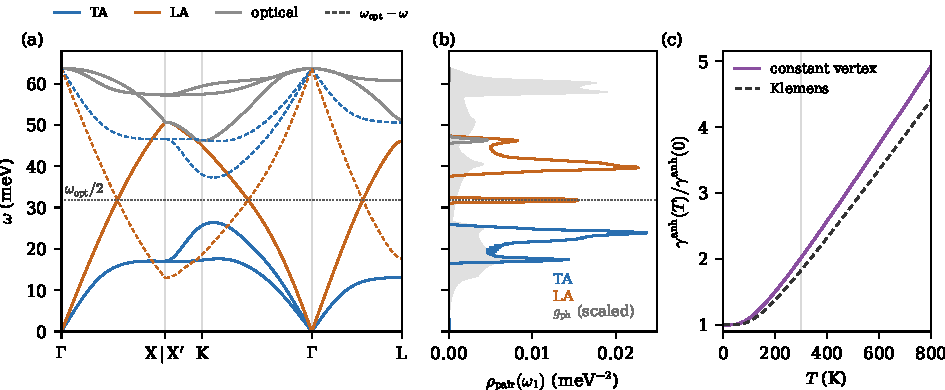
\includegraphics[width=\linewidth]{figures/ch05/fig5_6.pdf}
  \caption{Three-phonon decay of the zone-center optical phonon of silicon, $\omega_{\mathrm{opt}} = \SI{63.7}{meV}$ in this calculation. Phonons from the PBE force constants of \cref{fig:5-si} (DFPT on a $6^3$ grid of wavevectors, $a = \SI{5.431}{\angstrom}$), Fourier-interpolated; branches are labeled by energy order, the lowest two transverse acoustic (TA, blue), the third longitudinal acoustic (LA, orange), the upper three optical (gray). (a) Dispersion (solid) and the mirror curves $\omega_{\mathrm{opt}} - \omega_{\vect{Q}\nu}$ of the acoustic branches (dashed). A solid branch crossing a dashed one marks a pair $(\vect{Q},-\vect{Q})$ whose energies add to $\omega_{\mathrm{opt}}$; dotted: $\omega_{\mathrm{opt}}/2$. (b) Two-phonon density of final states resolved by the energy $\omega_1$ of one member of the pair and by its branch, $\rho_{\mathrm{pair}}(\omega_1) = N^{-1}\sum_{\vect{Q}\nu_1\nu_2}\delta(\omega_1 - \omega_{\vect{Q}\nu_1})\,\delta(\omega_{\mathrm{opt}} - \omega_{\vect{Q}\nu_1} - \omega_{\vect{Q}\nu_2})$, on an $80^3$ grid with Gaussians of width \SI{0.25}{meV} and a \SI{0.9}{meV} running mean; it is symmetric about $\omega_{\mathrm{opt}}/2$, each TA phonon (blue) pairing with an LA phonon (orange) at the mirror energy. Shaded: the one-phonon density of states $g_{\mathrm{ph}}$, scaled. LA+TA pairs make up \SI{89}{\percent} of the final states, LA+LA \SI{7}{\percent}, and TA+TA none; the remaining \SI{4}{\percent} are optical+TA pairs from a small region near K. (c) Temperature dependence of the width relative to $T = 0$: Klemens's law \cref{eq:5.7-klemens} (dashed) and the average of $1 + n_1 + n_2$ over the final states of panel (b) (solid), which assumes a constant vertex; the vertical line marks \SI{300}{K}.}
  \label{fig:5-decay}
\end{figure}

\begin{workedexample}{Klemens decay of the optical phonon of silicon}\label{we:5-klemens}
We compare the width of the zone-center optical phonon with the Klemens law \cref{eq:5.7-klemens}, using the measured $\omega_{\mathrm{opt}} = \SI{64.1}{meV}$.

\emph{The measured width.} At low temperature the Raman line of the mode has a full width of \SI{1.45}{cm^{-1}}~\cite{menendez1984temperature}, as tabulated in Ref.~\cite[Table~1]{debernardi1994anharmonic}. With $\SI{1}{cm^{-1}} = \SI{0.12398}{meV}$, this is $\gamma_{\mathrm{\Gamma},\mathrm{opt}} = \SI{0.180}{meV}$, and
\begin{equation*}
  \frac{\gamma_{\mathrm{\Gamma},\mathrm{opt}}}{\omega_{\mathrm{opt}}} = 2.80\times10^{-3} , \qquad
  \frac{1}{\gamma_{\mathrm{\Gamma},\mathrm{opt}}} = \SI{3.66}{ps} ,
\end{equation*}
57 periods of \SI{64.5}{fs}. Other measurements range from 1.24 to \SI{2.1}{cm^{-1}}~\cite{debernardi1994anharmonic}, a spread that reflects sample quality and spectral resolution. Silicon is an insulator, with $\gamma^{\mathrm{ep}}_{\vect{Q}\nu} = 0$ at low temperature, and isotope scattering is weak for a mode at the top of the spectrum. The width is anharmonic. A DFPT calculation of the full vertex \cref{eq:5.7-V3}, inserted in \cref{eq:5.7-gamma}, yields \SI{1.43}{cm^{-1}}~\cite[Table~1]{debernardi1994anharmonic}, \SI{99}{\percent} of the measured value, so three-phonon decay accounts for the whole width.

\emph{The temperature dependence.} At the \SI{10}{mK} of a detector, $\omega_{\mathrm{opt}}/2T = 3.7\times10^4$, the occupation $n_{\mathrm{B}}(\omega_{\mathrm{opt}}/2)$ is $\ee^{-37000}$, and the width is its zero-temperature value: the optical phonon decays spontaneously, with no help from thermal phonons. At \SI{77}{K}, $n_{\mathrm{B}}(\omega_{\mathrm{opt}}/2) = 0.008$ and the Klemens factor is 1.016. At \SI{300}{K}, $n_{\mathrm{B}}(\omega_{\mathrm{opt}}/2) = 0.407$, and \cref{eq:5.7-klemens} predicts
\begin{equation*}
  \gamma_{\mathrm{\Gamma},\mathrm{opt}}(\SI{300}{K}) = \SI{1.45}{cm^{-1}}\times(1 + 2\times0.407) = \SI{2.63}{cm^{-1}} .
\end{equation*}
With a constant vertex, averaging $1 + n_1 + n_2$ over the dominant asymmetric pairs gives a factor 2.01 instead of 1.82 and a width of \SI{2.92}{cm^{-1}} (\cref{fig:5-decay}(c)). The Klemens law thus gets the form of the temperature dependence right: a constant plus a term that grows as the Bose function of the daughters. Its single daughter energy, $\omega_{\mathrm{opt}}/2$, misses the true pairs of silicon, and at room temperature the Klemens law gives a width about \SI{10}{\percent} below the estimate from those pairs. With the full vertex and the true daughters, \cref{eq:5.7-gamma} follows the measured widths up to temperatures of the order of $\omega_{\mathrm{opt}} \approx \SI{740}{K}$~\cite{debernardi1994anharmonic}.

The Klemens law is a good parametrization of the temperature dependence once its zero-temperature width is taken from experiment or from a calculation. It does not predict that width, and its picture of the channel is wrong in silicon.
\end{workedexample}

\subsection{The anharmonic small parameter}

How large are the anharmonic terms compared with the harmonic ones? The natural measure is the ratio of the cubic to the harmonic energy at the zero-point amplitude of a mode. Take a bond-like coordinate with curvature $\Phi^{(2)}$, cubic coefficient $\Phi^{(3)}$ and zero-point length $\ell_{\mathrm{zp}}$. The ratio of $\tfrac16\Phi^{(3)}\ell_{\mathrm{zp}}^3$ to $\tfrac12\Phi^{(2)}\ell_{\mathrm{zp}}^2$ defines the \emph{anharmonic small parameter}
\begin{equation}
  \eta_{\mathrm{anh}} = \frac{|\Phi^{(3)}|\,\ell_{\mathrm{zp}}}{3\,\Phi^{(2)}} .
  \label{eq:5.7-eta}
\end{equation}
Equivalently, $\eta_{\mathrm{anh}}$ is the zero-point amplitude measured in units of the length $3\Phi^{(2)}/|\Phi^{(3)}|$ over which the force constants change by their own size. The counting of \cref{sec:5.1} estimates it at once. Force constants of every order scale as $\Phi^{(n)} \sim \alpha^2m_e/a_0^n$, and the zero-point amplitude as $\ell_{\mathrm{zp}} \sim \kappa_{\mathrm{BO}}a_0$, so
\begin{equation*}
  \eta_{\mathrm{anh}} \sim \frac{\alpha^2m_e/a_0^3}{\alpha^2m_e/a_0^2}\,\kappa_{\mathrm{BO}}a_0 = \kappa_{\mathrm{BO}} .
\end{equation*}
The anharmonic parameter is the Born--Oppenheimer parameter itself: the cubic term is smaller than a phonon energy by one power of $\kappa_{\mathrm{BO}}$, as \cref{sec:5.1} found. The quartic term, $\tfrac1{24}\Phi^{(4)}\ell_{\mathrm{zp}}^4$, is smaller than the harmonic one by $\eta_{\mathrm{anh}}^2$, since $\Phi^{(4)}\ell_{\mathrm{zp}}^2/\Phi^{(2)} \sim (\ell_{\mathrm{zp}}/a_0)^2$, and each further order brings one more power.

The physical effects follow by counting powers of $\eta_{\mathrm{anh}}$. The cubic term changes no energy at first order, since it is a product of an odd number of displacements and its average over any harmonic state vanishes. At second order it shifts the levels by $(\eta_{\mathrm{anh}}\omega_{\mathrm{ph}})^2/\omega_{\mathrm{ph}} = \eta_{\mathrm{anh}}^2\omega_{\mathrm{ph}}$, since the energy denominators of second-order perturbation theory are themselves phonon energies. The quartic term shifts them at first order by the same amount, $\eta_{\mathrm{anh}}^2\omega_{\mathrm{ph}}$. The decay rate \cref{eq:5.7-gamma} is the square of a cubic matrix element of size $\eta_{\mathrm{anh}}\omega_{\mathrm{ph}}$ times a density of final states of order $1/\omega_{\mathrm{ph}}$, again $\eta_{\mathrm{anh}}^2\omega_{\mathrm{ph}}$. The three effects are of one order:
\begin{equation}
  \frac{\gamma^{\mathrm{anh}}_{\vect{Q}\nu}}{\omega_{\vect{Q}\nu}} \sim \frac{\Delta\omega^{\mathrm{anh}}_{\vect{Q}\nu}}{\omega_{\vect{Q}\nu}} \sim \eta_{\mathrm{anh}}^2 \sim \kappa_{\mathrm{BO}}^2 ,
  \label{eq:5.7-order}
\end{equation}
where $\Delta\omega^{\mathrm{anh}}_{\vect{Q}\nu}$ is the anharmonic shift of the frequency. In absolute terms the shift and the width are $\alpha^2m_e\,\kappa_{\mathrm{BO}}^4$, the anharmonic level of the Born--Oppenheimer hierarchy of \cref{sec:5.1}. In the labeling of \cref{sec:8.5} the order $\eta_{\mathrm{anh}}^2$ is anharmonic order $n_A = 2$, where $n_A$ counts powers of the anharmonic expansion parameter in the response rather than vertices, and the leading anharmonic phonon self-energy is of that order. In thermal equilibrium the zero-point length is replaced by the thermal amplitude, $\ell_{\mathrm{zp}}^2 \to \ell_{\mathrm{zp}}^2(2n_{\mathrm{B}} + 1)$, as in \cref{eq:5.3-B}, and at high temperature $\eta_{\mathrm{anh}}^2$ grows in proportion to $T$, as the widths do.

Silicon bears out this counting. Along the bond coordinate of \cref{fig:5-scales}(c), $\Phi^{(2)} = \SI{13.6}{eV.\angstrom^{-2}}$, $\Phi^{(3)} = \SI{-41.5}{eV.\angstrom^{-3}}$ and $\ell_{\mathrm{zp}} = \SI{0.048}{\angstrom}$ give $\eta_{\mathrm{anh}} = 0.049$, against $\kappa_{\mathrm{BO}} = 0.067$; the length over which the force constants change is $3\Phi^{(2)}/|\Phi^{(3)}| = \SI{0.98}{\angstrom}$, about \SI{40}{\percent} of the bond. Then $\eta_{\mathrm{anh}}^2 = 2.4\times10^{-3}$. The quartic-to-harmonic ratio at the same amplitude, $\Phi^{(4)}\ell_{\mathrm{zp}}^2/12\Phi^{(2)}$ with $\Phi^{(4)} \approx \SI{40}{eV.\angstrom^{-4}}$, is $0.6\times10^{-3}$, a quarter of $\eta_{\mathrm{anh}}^2$, and the measured width of \cref{we:5-klemens} is $\gamma/\omega_{\mathrm{opt}} = 2.8\times10^{-3}$, 1.2 times $\eta_{\mathrm{anh}}^2$. The coefficients of the counting are close to one, between a quarter and two here and in the Born--Oppenheimer hierarchy of \cref{we:5-kappa}. Silicon at detector temperatures is a weakly anharmonic crystal, and its harmonic phonons are correct to a few parts in a thousand, well below the few-percent error of the functional (\cref{sec:5.2}).

The anharmonic parameter is not always small, and it grows with $\ell_{\mathrm{zp}}$. Light atoms have larger amplitudes, since $\ell_{\mathrm{zp}} \propto M^{-1/4}$ at fixed force constants, and hydrogen has $\kappa_{\mathrm{BO}} = 0.15$. The parameter also grows for soft modes near a structural instability, where $\Phi^{(2)} \to 0$ and the harmonic expansion about the minimum loses its meaning. The parameter is also large in quantum crystals such as solid helium, where the zero-point motion is a sizable fraction of the spacing, and in any crystal near melting. At low energy phonon decay is controlled by phase space rather than by $\eta_{\mathrm{anh}}$. The width of a long-wavelength acoustic phonon at $T = 0$ scales as the fifth power of its energy, and this width sets how fast the phonons that a dark-matter event leaves behind down-convert. For the nuclear response to dark matter, $\eta_{\mathrm{anh}}$ measures how far the harmonic results of this chapter can be trusted, and \cref{sec:11.5} turns it into a correction.

\subsection{Effective harmonic theories}

When temperature, light atoms or soft modes make the expansion \cref{eq:5.7-expand} converge slowly, the usual remedy is not to add orders but to find a better harmonic problem. Three effective harmonic theories are in common use, and they differ in what the harmonic force constants are fitted to.

The \emph{quasi-harmonic approximation} fits the force constants to the volume. It keeps every mode harmonic but computes the frequencies at the cell volume $\Omega$ that minimizes the free energy at temperature $T$, \cref{eq:E.8-qha}. The volume dependence of the frequencies is itself a cubic effect. A homogeneous strain $\epsilon$ displaces every nucleus by $u_i = \sum_\beta\epsilon^{\alpha_i\beta}X^\beta_i$, with $\vect{X}_i$ its equilibrium position. The force constants about the strained configuration then change, to first order, by
\begin{equation}
  \Phi^{(2)}_{ij}(\epsilon) - \Phi^{(2)}_{ij} = \sum_k\Phi^{(3)}_{ijk}\sum_\beta\epsilon^{\alpha_k\beta}X^\beta_k .
  \label{eq:5.7-strain}
\end{equation}
The Grüneisen parameter $\gamma^{\mathrm{G}}_{\vect{Q}\nu} = -\partial\ln\omega_{\vect{Q}\nu}/\partial\ln\Omega$ of \cref{sec:5.2} is therefore a projection of $\Phi^{(3)}$, and a harmonic crystal, with $\Phi^{(3)} = 0$, neither expands when heated nor shifts its phonons under pressure. The zero-point energy of \cref{sec:5.3} also depends on the volume, and the resulting zero-point pressure expands the lattice at $T = 0$ beyond the static minimum of \cref{sec:5.1}. The quasi-harmonic approximation keeps the cubic term at the level of the volume. It drops the shifts at fixed volume, which \cref{eq:5.7-order} puts at the same order, and it has no widths.

The \emph{self-consistent harmonic approximation} (SCHA) fits the force constants to the distribution of the nuclei, by a variational principle~\cite{errea2014anharmonic}. For any trial density matrix $\tilde\varrho$, the functional $\mathcal{F}[\tilde\varrho] = \langle H\rangle_{\tilde\varrho} - TS_{\mathrm{ent}}[\tilde\varrho]$ is an upper bound on the free energy (the Gibbs--Bogoliubov inequality). The SCHA takes for $\tilde\varrho$ the thermal state of a harmonic Hamiltonian $H_{\mathrm{trial}}$ with centroids $\bar X_a$ and auxiliary force constants $\Phi^{(2)}_{\mathrm{aux}}$, \cref{eq:E.8-scha}, with $a$ running over the Cartesian coordinates $X_a$ of all nuclei and $\delta X_a = X_a - \bar X_a$. The distribution of positions in this state is a Gaussian centered at $\bar X$. With $\mathcal{F}_{\mathrm{trial}}$ the free energy of $H_{\mathrm{trial}}$ and $V_{\mathrm{trial}} = \tfrac12\sum_{ab}\delta X_a\Phi^{(2)}_{\mathrm{aux},ab}\delta X_b$ its potential, the bound reads
\begin{equation*}
  \mathcal{F}[\tilde\varrho] = \mathcal{F}_{\mathrm{trial}} + \bigl\langle E^{\mathrm{ad}} - V_{\mathrm{trial}}\bigr\rangle_{\tilde\varrho} .
\end{equation*}
We minimize the bound. A change of $\Phi^{(2)}_{\mathrm{aux},ab}$ changes $\mathcal{F}_{\mathrm{trial}}$ by $\tfrac12\langle\delta X_a\delta X_b\rangle\,\delta\Phi^{(2)}_{\mathrm{aux},ab}$, the thermal form of the Hellmann--Feynman theorem of \cref{sec:5.1}, and the average of $V_{\mathrm{trial}}$ by the same amount plus $\tfrac12\sum_{cd}\Phi^{(2)}_{\mathrm{aux},cd}\,\delta\langle\delta X_c\delta X_d\rangle$. The first contributions cancel. The average of $E^{\mathrm{ad}}$ over a Gaussian depends on the force constants only through the covariance $\langle\delta X_c\delta X_d\rangle$, and a Gaussian obeys the diffusion equation in its covariance, so that $\delta\langle E^{\mathrm{ad}}\rangle = \tfrac12\sum_{cd}\langle\partial_c\partial_dE^{\mathrm{ad}}\rangle\,\delta\langle\delta X_c\delta X_d\rangle$. Altogether
\begin{equation*}
  \delta\mathcal{F} = \frac12\sum_{cd}\Bigl[\bigl\langle\partial_c\partial_dE^{\mathrm{ad}}\bigr\rangle_{\tilde\varrho} - \Phi^{(2)}_{\mathrm{aux},cd}\Bigr]\,\delta\langle\delta X_c\delta X_d\rangle ,
\end{equation*}
and the centroids enter only through $\langle E^{\mathrm{ad}}\rangle$, whose derivative is the average force. Both variations vanish at the minimum:
\begin{keyresult}[Self-consistent harmonic approximation]
\begin{equation}
  \Phi^{(2)}_{\mathrm{aux},ab} = \Bigl\langle\frac{\partial^2E^{\mathrm{ad}}}{\partial X_a\,\partial X_b}\Bigr\rangle_{\tilde\varrho} , \qquad
  \Bigl\langle\frac{\partial E^{\mathrm{ad}}}{\partial X_a}\Bigr\rangle_{\tilde\varrho} = 0 .
  \label{eq:5.7-scha}
\end{equation}
The auxiliary force constants are the curvature of the true energy surface averaged over the Gaussian distribution that they themselves generate, and the centroids lie where the average force vanishes.
\end{keyresult}
These are the stationarity conditions of Ref.~\cite[Eqs.~(21) and~(22)]{errea2014anharmonic}, which writes them as averages of forces. The first condition is self-consistent because the width of the distribution, $\langle\delta X_a\delta X_b\rangle$, is computed from the auxiliary frequencies with the zero-point and thermal factors of \cref{eq:5.3-B}. Expanded in the force constants, the average curvature is $\Phi^{(2)} + \tfrac12\sum_{cd}\Phi^{(4)}_{abcd}\langle\delta X_c\delta X_d\rangle + \cdots$: its first correction is the first-order quartic shift of \cref{eq:5.7-order}, and the SCHA sums this shift to all orders, together with the corrections from the higher even force constants. The cubic term enters only through the shift of the centroids and, in the physical phonon frequencies, through an added bubble term. For soft modes the SCHA is the right starting point even when the harmonic frequencies are imaginary, since the average curvature can be positive where the curvature at the minimum is not.

The \emph{temperature-dependent effective potential} fits the force constants to forces. It samples nuclear configurations at temperature $T$, by molecular dynamics, computes the forces in each, and finds the effective constants $\tilde\Phi^{(2)}$ that reproduce them best in the least-squares sense, \cref{eq:E.8-tdep}~\cite{hellman2011lattice}. For a Gaussian sample the least-squares fit returns exactly the average curvature of \cref{eq:5.7-scha}. The reason is that a Gaussian average of the force times a displacement is the average of the force's derivative times the covariance. The temperature-dependent effective potential and the SCHA differ in the distribution they sample, a classical one in molecular dynamics and a quantum Gaussian in the SCHA. That difference matters at detector temperatures, where a classical sample sees an almost static lattice and misses the zero-point motion. The same fit extends to effective third-order constants, from which \cref{eq:5.7-gamma} gives temperature-dependent widths~\cite{hellman2013temperature}.

For silicon at \SI{10}{mK}, all three effective harmonic theories reduce to the harmonic phonons of \cref{sec:5.2} with corrections of a few parts in a thousand, so the rest of the book can work with the harmonic phonons.

\section*{Summary}

Electrons are lighter than nuclei by a factor of about $2\times10^{-5}$ in silicon, and they settle into their ground state many times during one vibration of the lattice (\cref{sec:5.1}). The Born--Oppenheimer approximation turns their ground-state energy at fixed nuclei, with the repulsion of the nuclei added, into the potential-energy surface $E^{\mathrm{ad}}(u)$ on which the nuclei move. The small parameter is the fourth root of the mass ratio, $\kappa_{\mathrm{BO}} = (m_e/M)^{1/4} = 0.067$; in an insulator the ratio that controls the approximation is the phonon energy over the gap, 0.0548 in silicon.

Expanded to second order about its minimum, the energy surface defines the force constants $\Phi^{(2)}$ and the dynamical matrix $D^{\mathrm{dyn}}(\vect{Q})$, whose eigenvalues are the squared phonon frequencies $\omega^2_{\vect{Q}\nu}$ and whose eigenvectors are the polarizations $\vect{e}_{\kappa\nu}(\vect{Q})$ (\cref{sec:5.2}). Silicon has six branches up to \SI{64.1}{meV}, flat transverse acoustic branches that pile up states near \SI{17}{meV}, and no LO--TO splitting.

Quantized, each normal mode is an oscillator and a phonon is one of its quanta (\cref{sec:5.3}). Emitting a phonon has the weight $n_{\vect{Q}\nu} + 1$ and absorbing one the weight $n_{\vect{Q}\nu}$, and in a cryogenic detector every mode is empty, so emission is the whole signal. Zero-point motion alone spreads a silicon nucleus over \SI{0.05}{\angstrom} per Cartesian component.

In a polar crystal the sublattices carry Born effective charges $Z^*_\kappa$, which add up to zero; $Z^*_\kappa$ is the force on a nucleus per unit macroscopic field (\cref{sec:5.5}). The long-range field of a longitudinal optical wave splits the longitudinal from the transverse modes, in GaAs \SI{36.4}{meV} against \SI{33.6}{meV}, and the splitting gives $Z^* = 2.11$. A uniform field couples only to the polar optical modes at the zone center, through $Z^*_\kappa$, coherently in every cell.

At finite momentum transfer the response of a nucleus is controlled by thermal averages of exponentials of displacements (\cref{sec:5.6}). For a harmonic crystal the probability that the lattice absorbs $\vect{q}$ and stays in its state is the Debye--Waller factor $\ee^{-2W_\kappa}$, with $2W_\kappa = \vect{q}\cdot B_\kappa\cdot\vect{q}$, and the number of phonons created is a Poisson distribution with mean $2W_\kappa$. In silicon at zero temperature $2W_\kappa = 1$ at $q = \SI{40}{keV}$, the crossover from single phonons to multiphonon emission.

The cubic term of the energy surface lets a phonon decay into two (\cref{sec:5.7}); the zone-center optical phonon of silicon decays mainly into a transverse and a longitudinal acoustic phonon of unequal energies. The anharmonic small parameter $\eta_{\mathrm{anh}}$, the ratio of the cubic to the harmonic energy at the zero-point amplitude, is of order $\kappa_{\mathrm{BO}}$, 0.049 in silicon, and widths and anharmonic shifts are both of relative order $\eta_{\mathrm{anh}}^2$.

The phonons, their correlations and their lifetimes are all properties of the energy surface of electrons that never leave their ground state. The couplings that the Born--Oppenheimer approximation dropped let a moving nucleus excite the electrons, and a passing electron excite the lattice; \cref{chap:6} derives them.

\printbibliography[heading=subbibliography]
